\documentclass[handout, 9pt]{beamer}

\usetheme{Nantes}
\usepackage{src/drivers/config}

\title[Calculabilité et Complexité]{Calculabilité et Complexité}

\author[Matthieu Perrin]{
  Matthieu Perrin\\
  Laboratoire des Sciences du Numérique de Nantes \\
  UMR CNRS 6004\\
  Bureau 410, bâtiment 34 \\
  \url{matthieu.perrin@univ-nantes.fr}\\
}

\date{
  Nantes Université\\
  Licence d'Informatique, troisième année\\
  2025-2026
}

\hypersetup{
  pdftitle  = {Calculabilité et Complexité},
  pdfauthor = {Matthieu Perrin}
}

\begin{document}

\begin{frame}[plain,noframenumbering]
  \titlepage
  \on[text, bottom=-5mm]{\scriptsize
    \begin{description}
    \item[Licence :] \href{https://creativecommons.org/licenses/by-sa/4.0/}{CC BY-SA 4.0} (\ccbysa{}) — Matthieu Perrin
    \item[Code source :]\vspace{-.5mm}  \url{https://github.com/CalculabiliteEtComplexite/CM}
    \end{description}
  }
\end{frame}

% SPDX-License-Identifier: CC-BY-SA-4.0
% Author: Matthieu Perrin

\begingroup


\part{Introduction}
 
 
\section{Introduction}
 
\subsection{Langages et problèmes de décision}
% SPDX-License-Identifier: CC-BY-SA-4.0
% Author: Matthieu Perrin
% Part: <Nom de la partie>
% Section: <Nom de la section>
% Sub-section: <Nom de la sous-section>  % (facultatif, laisser vide si non utilisé)
% Frame: <Titre de la slide>

\begingroup

\begin{frame}{Reformulation du programme de Hilbert}

  \begin{block}{Le programme de Hilbert}
    Trouver un système de preuve $\langle \Phi, \Pi, \valid \rangle$ :
    \begin{itemize}
    \item cohérent et complet ; 
    \item suffisamment expressif pour formaliser les mathématiques ;
    \item tel que ces problèmes soient \alert{décidables par une procédure mécanique} :
    \end{itemize}

    \hspace\fill
    \begin{minipage}[t]{.45\textwidth}
      \begin{problembox}
        \textsc{Vérification des preuves}\\
        \structure{Instance :}
        \begin{itemize}
        \item Une preuve $\pi \in \Pi$ 
        \item Une proposition $\varphi \in \Phi$ 
        \end{itemize}
        \structure{Question :}
        \begin{itemize}
        \item Est-ce que $\pi \valid \varphi$ ?
        \end{itemize}
      \end{problembox}
    \end{minipage}
    \hspace\fill
    \begin{minipage}[t]{.5\textwidth}
      \begin{problembox}
        \textsc{Entscheidungsproblem}\\
        \structure{Instance :}
        \begin{itemize}
        \item Une proposition $\varphi \in \Phi$ 
        \end{itemize}
        \structure{Question :}
        \begin{itemize}
        \item Est-ce que $\exists \pi \in \Pi,   \pi \valid \varphi$ ?
        \end{itemize}
      \end{problembox}
    \end{minipage}
    \hspace\fill
  \end{block}
  
  \begin{center}
    \alert{Que signifie ``décidable par une procédure mécanique'' ?} 
  \end{center}

\end{frame}

\endgroup
\endinput

% SPDX-License-Identifier: CC-BY-SA-4.0
% Author: Matthieu Perrin
% Part: <Nom de la partie>
% Section: <Nom de la section>
% Sub-section: <Nom de la sous-section>  % (facultatif, laisser vide si non utilisé)
% Frame: <Titre de la slide>

\begingroup

\begin{frame}{Problème binaire et problème de décision}

  Un \structure{problème binaire} est une question dont la réponse est \alert{oui} ou \alert{non} en fonction de ses \structure{entrées}.

  \begin{exampleblock}{Exemples}
    \begin{itemize}
    \item \example{Primalité :} un entier est-il premier ?  
    \item \example{Classification :} une image donnée contient-elle un chat ? 
    \item \example{Base de données :} une requête donnée retourne-t-elle des résultats ?  
    \item \example{Sudoku :} une grille donnée peut-elle être remplie ? 
    \item \example{SAT :} une formule en forme normale conjonctive est-elle satisfiable ? 
    \item \example{Preuve :} un énoncé de théorème est-il démontrable dans une théorie ? 
    \item \example{Décision :} étant donnés un mot $u$ et un langage $L$, a-t-on $u\in L$ ? 
    \end{itemize}
  \end{exampleblock}
  
  \begin{alertblock}{Observations}
    \begin{itemize}
    \item En informatique, les entrées sont toujours encodables par des mots
    \item \alert{Les problèmes binaires sont encodés par des langages}
    \end{itemize}
  \end{alertblock}
  
\end{frame}

\endgroup
\endinput

\input{turing_machine/introduction/decision_problem/primality}
 
\subsection{La hiérarchie de Chomsky}
% SPDX-License-Identifier: CC-BY-SA-4.0
% Author: Matthieu Perrin
% Part: <Nom de la partie>
% Section: <Nom de la section>
% Sub-section: <Nom de la sous-section>  % (facultatif, laisser vide si non utilisé)
% Frame: <Titre de la slide>

\begingroup

\begin{frame}{Rappel : Grammaire non-restreinte}
  
  Une \structure{grammaire non-restreinte} est un quadruplet \alert{$\langle \Sigma, \Gamma, S, R \rangle$} tel que :
  \begin{description}
  \item[\alert{$\Sigma$}] alphabet : \structure{l'ensemble des terminaux}
  \item[\alert{$\Gamma$}] alphabet tel que $\Sigma \cap \Gamma = \emptyset$ : \structure{l'ensemble des non-terminaux}
  \item[\alert{$S$}] $\in \Gamma$ : \structure{l'axiome} (ou symbole initial)
  \item[\alert{$R$}] $\subseteq ((\Sigma \cup \Gamma)^\star \cdot \Gamma \cdot (\Sigma \cup \Gamma)^\star) \times (\Sigma \cup \Gamma)^\star$ : \\\structure{l'ensemble des règles de production}
  \end{description}

  \vfill
  Une \structure{règle de production} est un couple \alert{$\langle \alpha, \beta \rangle \in R$}, noté $\alert{\alpha \rightarrow \beta}$ tel que :
  \begin{description}
  \item[\alert{$\alpha$}] $\in (\Sigma \cup \Gamma)^\star \cdot \Gamma \cdot (\Sigma \cup \Gamma)^\star$ : \structure{membre gauche}
  \item[\alert{$\beta$}] $\in (\Sigma \cup \Gamma)^\star$ : \structure{membre droit}
  \end{description}

  \vfill
  On dit que :
  \begin{itemize}
  \item \structure{$u$ se dérive directement en $v$}, noté $\alert{u \vdash v}$, si :
    $$\alert{\exists \structure{x}, \structure{y} \in (\Sigma \cup \Gamma)^\star, \exists \example{\alpha \rightarrow \beta} \in R,
    u = \structure{x} \cdot \example{\alpha} \cdot \structure{y} \land v = \structure{x} \cdot \example{\beta} \cdot \structure{y}}$$
  \item \structure{$u$ se dérive en $v$}, si $\alert{u \vdash^\star v}$ où  $\vdash^\star$ est la fermeture transitive et réflexive de $\vdash$.
  \end{itemize}

\end{frame}

\endgroup

\input{turing_machine/introduction/chomsky_hierarchy/hierarchy}
% SPDX-License-Identifier: CC-BY-SA-4.0
% Author: Matthieu Perrin
% Part: 
% Section: 
% Sub-section: 
% Frame: 

\begingroup

\begin{frame}{Grammaires et langages rationnels}

  \vspace{-2mm}
  \begin{block}{Définition -- Grammaire rationnelle}
    Soit \alert{$G = \langle \Sigma, \Gamma, S, \rightarrow \rangle$} une grammaire algébrique. 
    \begin{itemize}
    \item $G$ est dite \structure{rationnelle à droite} si ses règles sont de la forme :
      \begin{center}
        $\alert{A \rightarrow a \cdot B}$ \quad ou\quad $\alert{A \rightarrow a}$ \quad ou\quad $\alert{A \rightarrow \varepsilon}$
        \quad avec \structure{$A, B \in \Gamma$} et \structure{$a\in \Sigma$}
      \end{center}
    \item $G$ est dite \structure{rationnelle à gauche} si ses règles sont de la forme :
      \begin{center}
        $\alert{A \rightarrow B \cdot a}$ \quad ou\quad $\alert{A \rightarrow a}$ \quad ou\quad $\alert{A \rightarrow \varepsilon}$
        \quad avec \structure{$A, B \in \Gamma$} et \structure{$a\in \Sigma$}
      \end{center}
    \item $G$ est dite \structure{rationnelle} si elle est \structure{rationnelle à droite ou à gauche}
    \end{itemize}
  \end{block}

  \vspace{-1mm}
  \begin{block}{Définition -- Langage rationnel}
    \vspace{-1mm}
    Soient $\Sigma$ un alphabet et $L$ un langage sur $\Sigma$.
    \begin{itemize}
    \item On dit que $L$ est \structure{rationnel} s'il est engendré par une grammaire rationnelle
    \item L'\structure{ensemble des langages rationnels} sur $\Sigma$ est noté \alert{$\textsc{rat}_\Sigma$}
    \item La \structure{classe des langages rationnels} est noté \alert{$\textsc{rat}$} (indépendant de $\Sigma$)
    \end{itemize}
  \end{block}

  \vspace{-1mm}
  \begin{exampleblock}{Exemple -- Langage $\{a^m b^n \mid m, n > 0\}$}
  \vspace{-1mm}
    \begin{itemize}
    \item $G = \langle \{a, b\}, \{S, T\}, S, \left\{S \rightarrow a S \mid a T ; T \rightarrow b T \mid b \right\} \rangle $
    \end{itemize}
  \end{exampleblock}

\end{frame}

\endgroup
\endinput

% SPDX-License-Identifier: CC-BY-SA-4.0
% Author: Matthieu Perrin
% Part: 
% Section: 
% Sub-section: 
% Frame: 

\begingroup

\begin{frame}{Grammaires et langages algébriques}

  \begin{block}{Définition -- Grammaire algébrique}
    Une grammaire $G = \langle \Sigma, \Gamma, S, \rightarrow \rangle$ est dite \structure{algébrique} si les membres gauches de toutes ses règles sont un non-terminal :

    $$\forall \langle \alpha, \beta\rangle \in \rightarrow, \quad \alert{\alpha \in \Gamma}$$
  \end{block}

  \vspace{-2mm}
  \begin{block}{Définition -- Langage algébrique}
    Soient $\Sigma$ un alphabet et $L$ un langage sur $\Sigma$.
    \begin{itemize}
    \item $L$ est dit \structure{algébrique} s'il est engendré par une grammaire algébrique
    \item L'\structure{ensemble des langages algébrique} sur $\Sigma$ est noté \alert{$\textsc{alg}_\Sigma$}
    \item La \structure{classe des langages algébrique} est noté \alert{$\textsc{alg}$} (indépendant de $\Sigma$)
    \end{itemize}
  \end{block}

  \begin{exampleblock}{Exemple -- Langage $\{a^n b^n \mid n\in \mathbb{N}\}$}
    \begin{itemize}
    \item $G = \langle \{a, b\}, \{S\}, S, \left\{S \rightarrow a S b \mid \varepsilon \right\} \rangle $
    \item Génération de $aabb$ : $ S \vdash aSb \vdash aaSbb \vdash aabb $
    \end{itemize}
  \end{exampleblock}
  
\end{frame}

\endgroup
\endinput

% SPDX-License-Identifier: CC-BY-SA-4.0
% Author: Matthieu Perrin
% Part: <Nom de la partie>
% Section: <Nom de la section>
% Sub-section: <Nom de la sous-section>  % (facultatif, laisser vide si non utilisé)
% Frame: <Titre de la slide>

\begingroup

\begin{frame}{Hiérarchie de chomsky et automates}

  \centering
  \begin{tikzpicture}[2Darray, x=25mm, y=17mm]
    \arrayColumn[width=8mm, header=Type]{
      \arrayLine{0}
      \arrayLine{1}
      \arrayLine{2}
      \arrayLine{3}
    }
    
    \arrayColumn[header=Grammaire]{
      \arrayLine{Non-restreinte\\ $\alpha A \beta \rightarrow \gamma$}
      \arrayLine{Contextuelle\\   $\alpha A \beta \rightarrow \alpha \gamma \beta$ \\ $\gamma\neq\varepsilon$}
      \arrayLine{Algébrique\\     $A \rightarrow \beta$}
      \arrayLine{Rationnelle\\    $A \rightarrow a B \mid b \mid \varepsilon$}
    }
    
    \arrayColumn[header=Langage]{
      \arrayLine{Récursivement\\ énumérable}
      \arrayLine{Contextuel}
      \arrayLine{Algébrique}
      \arrayLine{Rationnel}
    }
    
    \arrayColumn[header=Automate]{
      \arrayLine{Machine\\de Turing}
      \arrayLine{Automate\\linéairement\\ borné}
      \arrayLine{Automate à pile\\non déterministe}
      \arrayLine{Automate fini}
    }
    
    \arrayColumn[header=Déterminisable]{
      \arrayLine{Oui, mais \\complexité inconnue\\ \footnotesize $\textsc{p} \stackrel{?}{=} \textsc{np}$}
      \arrayLine{Inconnu\\ \footnotesize $\textsc{nspace}(\mathcal{O}(n))$ \\ $\stackrel{?}{=}$\\$\textsc{dspace}(\mathcal{O}(n))$}
      \arrayLine{Impossible}
      \arrayLine{Oui,\\ exponentiel\\ en nombre\\ d'états}
    }
  \end{tikzpicture}

  \begin{block}{Automates finis généralisés}
    Si un automate fini n'est pas suffisant, ajouter une structure de données
    \begin{itemize}
    \item Pile : \structure{automate à pile}
    \item Tableau de taille $|u|$ : \structure{automate linéairement bornée}
    \item Mémoire infini : \structure{machine de Turing}
    \begin{itemize}
    \item Quel modèle de mémoire permet de modéliser les algorithmes ? 
    \end{itemize}
    \end{itemize}
  \end{block}
  
\end{frame}

\endgroup

% SPDX-License-Identifier: CC-BY-SA-4.0
% Author: Matthieu Perrin
% Part: <Nom de la partie>
% Section: <Nom de la section>
% Sub-section: <Nom de la sous-section>  % (facultatif, laisser vide si non utilisé)
% Frame: <Titre de la slide>

\begingroup

\begin{frame}{Alan Turing}

  \onImage[x=-.25\textwidth,y=2mm]{%
    height=6cm,
    title={Alan Turing},
    license={Domaine public UK (1951, \href{https://commons.wikimedia.org/wiki/File:Alan_Turing_(1951).jpg}{Wikimedia})},
    img={Turing.jpg}
  }

  \onImage[x=.25\textwidth,y=2mm]{%
    height=6cm,
    title={The Imitation Game (2015)},
    license={$\copyright~2015$ - The Weinstein Company. Utilisation non commerciale à des fins pédagogiques (fair use)},
    img={imitation_game.jpg}
  }
  
\end{frame}

\endgroup

% SPDX-License-Identifier: CC-BY-SA-4.0
% Author: Matthieu Perrin
% Part: <Nom de la partie>
% Section: <Nom de la section>
% Sub-section: <Nom de la sous-section>  % (facultatif, laisser vide si non utilisé)
% Frame: <Titre de la slide>

\begingroup

\begin{frame}{Thèse de Church -- Turing}

  \onBlock[left=.75\textwidth, y=22mm]{Thèse de Church -- Turing (1936-1937)}{
    \centering
    \structure{La définition des \og fonctions calculables \fg par des \\
      \alert{Machines de Turing déterministes}  \\
      caractérise la notion intuitive de \og procédure effective \fg.}
  }
  
  \onBlock[y=-15mm]{Arguments en faveur de la thèse}{
    \begin{itemize}
    \item Équivalence entre formalismes
      \begin{itemize}
      \item Machines de Turing, $\lambda$-calcul, langages de programmation...
      \end{itemize}
    \item On ne connaît pas de machine plus puissante 
      \begin{itemize}
      \item Les formalismes plus expressifs necessitent des \og oracles \fg
        \begin{itemize}
        \item Par exemple, on peut \emph{définir} des objets mathématiques non-calculables
        \end{itemize}
      \item Les limites au formalisme sont internes
        \begin{itemize}
        \item L'indécidabilité du \structure{problème de l'arrêt} vient d'un paradoxe
        \end{itemize}
      \end{itemize}
    \item Possibilité de simuler l'univers...
      \begin{itemize}
      \item ... donc toute machine qui peut y être effectivement construite 
      \end{itemize}
    \end{itemize}
  }

  \onImage[x=42mm,y=15mm]{%
    width=2.3cm,
    title={Alonzo Church},
    license={$\copyright$ - Princeton University Library (voir \href{https://en.wikipedia.org/wiki/File:Alonzo_Church.jpg}{Wikimedia}). Utilisation non commerciale à des fins pédagogiques (fair use)},
    img={Church.jpg}
  }

\end{frame}



\endgroup

% SPDX-License-Identifier: CC-BY-SA-4.0
% Author: Matthieu Perrin
% Part: 
% Section: 
% Sub-section: 
% Frame: 

\begingroup

\begin{frame}{Comment modéliser la mémoire ?}

  \begin{block}{Modèle de processus dans les OS}
    \begin{itemize}
    \item \structure{Mémoire disponible : }
      \begin{itemize}
      \item Un tableau de $2^N$ octets.
      \item Des pointeurs sur $N$ bits.
        \begin{itemize}
        \item Typiquement, $N=32$ ou $N=64$.
        \end{itemize}
      \end{itemize}
    \item \alert{Problème :} 
      \begin{itemize}
      \item En théorie, un automate fini à $2^{2^N}$ états
        \begin{itemize}
        \item En pratique, $N$ fini et $2^N$ infini
        \end{itemize}
      \end{itemize}
    \end{itemize}
  \end{block}
  \pause
  \begin{block}{Modèle RAM (\emph{Random access machine})}
    \begin{itemize}
    \item \structure{Mémoire disponible : }
      \begin{itemize}
      \item Un tableau infini d'entiers non-bornés.
      \end{itemize}
    \item \alert{Problème :} 
      \begin{itemize}
      \item Il faut des opérations sur les entiers dans le modèle
        \begin{itemize}
        \item Ces opérations ne sont-elles pas déjà des algorithmes ?
        \item On veut un \structure{ensemble de règles fini}.
        \end{itemize}
      \end{itemize}
    \end{itemize}
  \end{block}
\end{frame}

\endgroup

 
 
\part{Calculabilité}
 
 
\section{Machines de Turing Déterministes}
 
\subsection{Définition des machines de Turing}
% SPDX-License-Identifier: CC-BY-SA-4.0
% Author: Matthieu Perrin
% Part: 
% Section: 
% Sub-section: 
% Frame: 

\begingroup

\begin{frame}{Un automate à ruban}

  \on[text,top]{
    \begin{itemize}
    \item Une \structure{machine de Turing} est un \alert{automate} à \alert{ruban}.
      \begin{itemize}
      \item en : ``\structure{\textit{Infinite tape}}'' = fr : \og \structure{\textit{ruban infini}} \fg
      \item en : ``\structure{\textit{Magnetic tape}}'' = fr : \og \structure{\textit{bande magnétique}} \fg
      \end{itemize}
    \end{itemize}
  }

  \onImage[y=4mm]{%
    height=2.2cm,
    title={Cassette VHS},
    license={{}\ccbysa{} \href{https://creativecommons.org/licenses/by-sa/4.0/}{CC BY-SA 4.0} -- Toby Hudson 2012 -- \href{https://commons.wikimedia.org/wiki/File:VHS_cassette_tape_12.JPG}{Wikimedia}},
    img={vhs.jpg}
  }
  
  \on[text,bottom=3mm]{
    \begin{itemize}
    \item Exécution du \structure{contrôleur} :
      \begin{itemize}
      \item Un \structure{automate fini} décide des opérations sur la mémoire
      \item L'exécution dure aussi longtemps qu'il y a des actions possibles
      \end{itemize}
    \item Opérations sur le \structure{ruban} :
      \begin{itemize}
      \item \alert{Lire/écrire} à la position de la tête de lecture/écriture
      \item \alert{Déplacer} la tête de lecture/écriture vers la gauche ou vers la droite
      \item Pour simplifier : une lecture, une écriture, et un déplacement par étape
      \end{itemize}
    \end{itemize}
  }
  
\end{frame}

\endgroup

% SPDX-License-Identifier: CC-BY-SA-4.0
% Author: Matthieu Perrin
% Part: 
% Section: 
% Sub-section: 
% Frame: 

\begingroup

\begin{frame}{Exemple : le \og busy beaver \fg}
  
  \on[top=4mm] {
    \begin{tikzpicture}[tape]
      \cell{0}
      \cell[alert ob=<{6}>       ]{\alt<-6> {0}{1}} \smheadb<6>
      \cell[alert ob=<{5,7}>     ]{\alt<-5> {0}{1}} \smheadb<5,7>
      \cell[alert ob=<{4,8}>     ]{\alt<-4> {0}{1}} \smheadb<4,8>
      \cell[alert on=<{1,3,9,13}>]{\alt<-1> {0}{1}} \smhead<1,3,9,13>
      \cell[alert ob=<{2,10,12}> ]{\alt<-2> {0}{1}} \smheadb<2,10,12>
      \cell[alert ob=<{11}>      ]{\alt<-11>{0}{1}} \smheadb<11>
      \cell{0}
    \end{tikzpicture}
  }
  
  \on[y=-6mm]{
    \begin{tikzpicture}[turingMachine, x=13mm, y=20mm]
      \state[alert on=<{1,3,6,12}>, initial] (a) at (0, 1) {$A$};
      \state[alert ob=<{2,5,7-11}>         ] (b) at (2, 1) {$B$};
      \state[alert ob=<{4,13}>,   accepting] (c) at (1, 0) {$C$};
      
      \path[alert on=<{1,6}>   ] (a) edge[bend left]  node       {\smTMtransR{0}{1}} (b);
      \path[alert ob=<{3,12}>  ] (a) edge[bend right] node[swap] {\smTMtransL{1}{1}} (c);
      \path[alert ob=<{2,5,11}>] (b) edge[bend left]  node       {\smTMtransL{0}{1}} (a);
      \path[alert ob=<{7-10}>  ] (b) edge[loop right] node       {\smTMtransR{1}{1}} (b);
      \path[alert ob=<{4}>     ] (c) edge[bend right] node[swap] {\smTMtransL{0}{1}} (b);
    \end{tikzpicture}
  }
 
  \on[text,bottom] {\footnotesize
    \begin{description}
    \item[$A \xrightarrow{\smTMtransR{0}{1}} B$ :] si on lit $0$ dans l'état $A$, écrire $1$, aller en $B$ et se déplacer à droite\vspace{-2mm}
    \item[$B \xrightarrow{\smTMtransL{0}{1}} A$ :] si on lit $0$ dans l'état $B$, écrire $1$, aller en $A$ et se déplacer à gauche
    \end{description}
  }

\end{frame}

\endgroup

\input{turing_machine/non_deterministic/definition/ndtm}
% SPDX-License-Identifier: CC-BY-SA-4.0
% Author: Matthieu Perrin
% Part: 
% Section: 
% Sub-section: 
% Frame: 

\begingroup

\begin{frame}{Configurations d'une machine de Turing}

  \onBlock[top=-5mm]{Définition -- Configuration d'une machine de Turing}{
    Soit $M=\langle \Sigma, \Gamma, \blank , Q, q_0, F, \rightarrow \rangle$ une machine de Turing.\\
    Une \structure{configuration} de $M$ est représentée par un triplet \alert{$\langle G, q, D \rangle$} tel que :
    \begin{description}[xxxx]
    \item[\alert{$G$}] $\in \Gamma^\star$ : le mot à \structure{gauche} de la tête (excluant la case sous la tête)
    \item[\alert{$q$}] $\in Q$ : \structure{l'état courant dans la simulation}
    \item[\alert{$D$}] $\in \Gamma^\star$ : le mot à \structure{droite} de la tête (incluant la case sous la tête)
    \end{description}
  }
  
  \onExampleBlock{Exemple -- La configuration {\color{black}$\langle \structure{ba},\alert{1},\example{ab}\rangle $}}{}

  \on[x=-29mm,y=-11mm] {
    \begin{tikzpicture}[tape, x=7mm, y=7mm]
      \cell{}
      \cell[structure]{$b$}  
      \cell[structure]{$a$}  
      \cell[example]  {$a$} \smhead[example]
      \cell[example]  {$b$}  
      \cell{} 
    \end{tikzpicture}
  }
 
  \on[x=29mm,y=-10mm] {
    \begin{tikzpicture}[turingMachine]
      \state[initial  ] (0) at (0,0) {0}; 
      \state[alert    ] (1) at (1,0) {1}; 
      \state[accepting] (2) at (2,0) {2}; 
      
      \path (0) edge[bend left] node {\smTMtransR{a}{b}} (1);
      \path (1) edge[bend left] node {\smTMtransR{a}{b}} (0);
      \path (1) edge            node {\smTMtransL{b}{a}} (2);
    \end{tikzpicture}
  }

  \onBlock[bottom=-1mm]{Remarque -- Modélisation des symboles blancs}{
    L'infinité de symboles blancs est modélisée par la \structure{relation d'équivalence} :\\[-2mm]
    $$\forall n, m\in \mathbb{N},\quad\structure{\langle G, q, D \rangle \alert{\,\simeq\,} \langle \alert{\blank ^n} G, q, D \alert{\blank ^m} \rangle}$$
    On note {\small\alert{$\mathcal{C}_M \eqdef (\Gamma^\star \times Q \times \Gamma^\star)/_\simeq$}} l'\structure{ensemble des configurations de $M$}
  }

  
\end{frame}

\endgroup

% SPDX-License-Identifier: CC-BY-SA-4.0
% Author: Matthieu Perrin
% Part: 
% Section: 
% Sub-section: 
% Frame: 

\begingroup

\begin{frame}{Actions d'une machine de Turing}
  
  \onBlock[top=-4mm]{Définition -- Action}{
    Soit $M=\langle \Sigma, \Gamma, \blank, Q, q_0, F, \rightarrow \rangle$ une machine de Turing. \\
    Les \structure{actions} de $M$ composent une relation binaire \alert{$\leadsto_M$}\footnote{On note \alert{$C \leadsto C'$} si $M$ est clair d'après le contexte.} sur $\mathcal{C}_M$\\
    Pour tous $q, q' \in Q$, $a, b, c \in \Gamma$, et $G, D \in \Gamma^\star$, on a :

    \vspace{-3mm}
    $$
    \begin{array}{@{\langle\,}l@{,\,}c@{,\,}r@{\,\rangle \leadsto_M \langle\,}l@{,\,}c@{,\,}r@{\,\rangle\quad\text{si}\quad}l}
      G           & \structure{q} & \alert{a} D   & G \alert{b} & \structure{q'} &  D   & \structure{q \xrightarrow{\alert{\smTMtransR{a}{b}}} q'}\\
      G \alert{c} & \structure{q} & \alert{a} D   & G           & \structure{q'} & \alert{cb} D   & \structure{q \xrightarrow{\alert{\smTMtransL{a}{b}}} q'}\\
    \end{array}
    $$
    
    On note \alert{$\leadsto_M^\star$} \structure{la fermeture transitive et réflexive de $\leadsto_M$}.
  }

  \onExampleBlock[text,y=-9mm] {Exemple -- $\structure{\langle b,1,aab\rangle} \leadsto \alert{\langle bb,0,ab\rangle}$} {}

  \on[x=-29mm,y=-19mm] {
    \begin{tikzpicture}[tape, x=6mm, y=6mm]
      \cell{}
      \cell{$b$}  
      \cell[structure]{$a$} \smhead[structure] 
      \cell{$a$}
      \cell{$b$} 
      \cell{}
    \end{tikzpicture}
  }

  \on[x=29mm,y=-19mm] {
    \begin{tikzpicture}[tape, x=6mm, y=6mm]
      \cell{}
      \cell{$b$}  
      \cell[alert]{$b$}
      \cell{$a$} \smheadfrom[example]{-1} \smhead[alert]
      \cell{$b$} 
      \cell{}
    \end{tikzpicture}
  }
  
  \on[x=-29mm,y=-32mm] {
    \begin{tikzpicture}[turingMachine]
      \state[initial  ] (0) at (0,0) {0}; 
      \state[structure] (1) at (1,0) {1}; 
      \state[accepting] (2) at (2,0) {2}; 
      
      \path          (0) edge[bend left=15] node {\smTMtransR{a}{b}} (1);
      \path[example] (1) edge[bend left=15] node {\smTMtransR{a}{b}} (0);
      \path          (1) edge               node {\smTMtransL{b}{a}} (2);
    \end{tikzpicture}
  }
  
  \on[x=29mm,y=-32mm] {
    \begin{tikzpicture}[turingMachine]
      \state[initial,alert] (0) at (0,0) {0}; 
      \state[             ] (1) at (1,0) {1}; 
      \state[accepting    ] (2) at (2,0) {2}; 
      
      \path          (0) edge[bend left=15] node {\smTMtransR{a}{b}} (1);
      \path[example] (1) edge[bend left=15] node {\smTMtransR{a}{b}} (0);
      \path          (1) edge               node {\smTMtransL{b}{a}} (2);
    \end{tikzpicture}
  }

  
\end{frame}

\endgroup

% SPDX-License-Identifier: CC-BY-SA-4.0
% Author: Matthieu Perrin
% Part: 
% Section: 
% Sub-section: 
% Frame: 

\begingroup

\begin{frame}{Exécution d'une machine de Turing}
  
  \vspace{-1mm}Soient $M=\langle \Sigma, \Gamma, \blank, Q, q_0, F, \rightarrow \rangle$ une machine de Turing, $u\in \Sigma^\star$.
 
  \begin{block}{Définitions -- Configurations remarquables}
    Une configuration $c = \langle G, q, D \rangle \in \mathcal{C}_M$ est dite :
    \begin{description}[s'arrête sur $u$ :]
    \item[initiale :] si $G = \varepsilon$ et $q = q_0$
      \hspace\fill{$\alert{C_{\mathit{init}}(u) \eqdef \langle \varepsilon, q_0, u \rangle}$}
    \item[d'arrêt :] si elle ne permet aucune action
      \hspace\fill{$\alert{\mathcal{C}_M^{\mathit{halt}} \eqdef \left\{c\in \mathcal{C}_M \,\middle\mid\, \nexists c', c\leadsto_M c'\right\}}$}
    \item[acceptante :] si $c\in \mathcal{C}_M^\mathit{halt}$ et $q \in F$
      \hspace\fill{$\alert{\mathcal{C}_M^+ \eqdef \left\{\langle G, q, D \rangle \in \mathcal{C}_M^\mathit{halt} \,\middle\mid\, q\in F\right\}}$}
    \end{description}
  \end{block}
 
  \begin{block}{Définitions -- Exécution de $M$ sur $u$}
    On dit que $M$ :
    \begin{description}[s'arrête sur $u$ :]
    \item[s'arrête sur $u$ :] si $M$ atteint une configuration d'arrêt
      \hspace\fill{$\alert{\exists c\in \mathcal{C}_M^\mathit{halt}, C_{\mathit{init}}(u) \leadsto_M^\star c}$}
    \item[accepte $u$ :] si $M$ atteint une config. acceptante
      \hspace\fill{$\alert{\exists c\in \mathcal{C}_M^+, C_{\mathit{init}}(u) \leadsto_M^\star c}$}
    \item[s'arrête :] si $M$ s'arrête sur toute entrée
      \hspace\fill{$\alert{\forall u\in\Sigma^\star, \exists c\in \mathcal{C}_M^\mathit{halt}, C_{\mathit{init}}(u) \leadsto_M^\star c}$}
    \end{description}

    Le \structure{langage accepté par $M$} est l'ensemble des mots acceptés par $M$\\[-2mm]
    $$\alert{\mathcal{L}(M) \eqdef \left\{u \in \Sigma^\star \;\middle\mid\; \exists c \in \mathcal{C}_M^+, C_{\mathit{init}}(u) \leadsto_M^\star c\right\}}$$
  \end{block}

\end{frame}

\endgroup

 
\subsection{Machines de Turing déterministes}
% SPDX-License-Identifier: CC-BY-SA-4.0
% Author: Matthieu Perrin
% Part: <Nom de la partie>
% Section: <Nom de la section>
% Sub-section: <Nom de la sous-section>  % (facultatif, laisser vide si non utilisé)
% Frame: <Titre de la slide>

\begingroup

\begin{frame}{Machine de Turing déterministe (MTD)}

  Soit $M = \langle \Sigma, \Gamma, \blank, Q, q_0, F, \rightarrow \rangle$ une MTND.
  \begin{block}{Définition -- Machine de Turing déterministe}
    On dit que $M$ est \structure{déterministe}
    si sa relation de transition $\rightarrow$ est fonctionnelle :

    $$\forall \alert{q}\in Q, \forall \alert{a}\in \Gamma,
    \left|\left\{
    \left\langle \structure{q'}, \structure{b}, \structure{d}\right\rangle \in Q \times \Gamma \times \{\triangleleft, \triangleright\}
    \;\middle\mid\;
    \alert{q} \xrightarrow{\smTMtrans{\alert{a}}{\structure{b}}{\structure{d}}} \structure{q'}
    \right\}\right|
    \le 1$$
  \end{block}
  
  \begin{block}{Remarques -- Notion de machine de Turing non-déterministe}
    \begin{itemize}
    \item Toute machine de Turing déterministe est une MTND
    \item \alert{``Non-déterministe''} signifie \alert{``pas forcément déterministe''}
    \end{itemize}
  \end{block}

\end{frame}

\endgroup

% SPDX-License-Identifier: CC-BY-SA-4.0
% Author: Matthieu Perrin
% Part: 
% Section: 
% Sub-section: 
% Frame: 

\begingroup

\begin{frame}{Machine de Turing non-déterministe}
  
  \onBlock[top=-4mm]{Rappel -- Machine de Turing déterministe}{
    Soit $M = \langle \Sigma, \Gamma, \blank, Q, q_0, F, \rightarrow \rangle$ une machine de Turing.
    \begin{itemize}
    \item $M$ est \structure{déterministe} si sa relation de transition $\rightarrow$ est fonctionnelle.
    \item \alert{``Non-déterministe''} signifie \alert{``pas forcément déterministe''}.
    \end{itemize}
    \begin{description}[Ubiquité :]
    \item[Modèle :] on autorise le modèle étendu (multi-ruban, immobilité, réécriture)
    \item[Ubiquité :] si non-déterminisme, un \structure{oracle} \alert{\emph{devine}} la meilleure transition
    \end{description}
  }
  
  \onBlock<2->[y=-9mm]{Comment utiliser le non-déterminisme ?}{
    \begin{itemize}
    \item Déplacement à un endroit \alert{arbitraire} du ruban
    \item Écriture d'un mot \example{arbitraire} sur le ruban
    \item Choix \structure{arbitraire} d'une sous-machine à exécuter
    \end{itemize}
  }

  \on<2->[x=40mm, y=-10mm] {
    \begin{tikzpicture}[turingMachine, x=15mm, y=8mm]\scriptsize
      \state[alert]     (01) at (0,1) {\faRandom}; 
      \state[example]   (11) at (1,1) {\faRandom}; 
      \state[example]   (21) at (2,1) {\faCheck}; 
      \state[structure] (00) at (0,0) {$A$}; 
      \state[structure] (10) at (1,0) {\faRandom}; 
      \state[structure] (20) at (2,0) {$B$}; 

      \path (01) edge[loop above] node  {\smAlign{\smTMtransR{x}{x}\smTMtransL{x}{x}}} (01);
      \path (11) edge[loop above] node  {\smAlign{\smTMtransL{\blank}{a}\smTMtransL{\blank}{b}}} (11);
      \path (11) edge node  {\smTMtransR{\blank}{\blank}} (21);

      \path (10) edge node  {\smTMtransS{\varepsilon}{\varepsilon}} (20);
      \path (10) edge node[swap] {\smTMtransS{\varepsilon}{\varepsilon}} (00);

      \node at (2,2) {$\forall x\in \Sigma$}; 
    \end{tikzpicture}
  }
  
  \onBlock<2->[y=-20mm, left=.48\textwidth, anchor=north]{Reconnaître un langage $L$}{
    \begin{description}[Entrée :]
    \item[Entrée :] $u\in \Sigma^\star$ 
    \item[Sortie :] \alert{une} exécution $\cmark{}$ si $u\in L$
    \end{description}
  }
  
  \onBlock<2->[y=-20mm, right=.48\textwidth, anchor=north]{Générer un langage $L$}{
    \begin{description}[Entrée :]
    \item[Entrée :] le mot vide $\varepsilon$ 
    \item[Sortie :] \alert{un} mot arbitraire de $L$
    \end{description}
  }

\end{frame}

\endgroup

% SPDX-License-Identifier: CC-BY-SA-4.0
% Author: Matthieu Perrin
% Part: <Nom de la partie>
% Section: <Nom de la section>
% Sub-section: <Nom de la sous-section>  % (facultatif, laisser vide si non utilisé)
% Frame: <Titre de la slide>

\begingroup

\begin{frame}{Langage décidable}

  \onBlock[top=-4mm]{Définition -- Décision d'un langage}{
    Soient $M=\langle \Sigma, \Gamma, \blank, Q, q_0, F, \rightarrow \rangle$ une MTD, $u\in \Sigma^\star$ et $L\subseteq \Sigma^\star$.
    \begin{itemize}
    \item On dit que \structure{$M$ décide $L$} si \alert{$L = \mathcal{L}(M)$} et \alert{$M$ s'arrête sur toutes ses entrées}
    \item On dit que \structure{$L$ est décidable} s'il existe une MTD qui décide $L$
    \item On note \alert{\textsc{r}} (pour \structure{récursif}) la classe des langages décidables
    \end{itemize}
  }

  \onExampleBlock[y=5mm]{Exemple -- Décision de $\{a^n b^n c^n \mid n > 0 \}$}

  \on[y=-4mm] {
    \begin{tikzpicture}[tape, x=7mm, y=7mm]%
      \cell{}
      \cell{}
      \cell{\alt<-1>{$a$}{$A$}} \smhead[alert]<1>      \smheadfromb[alert]<4>{3}  
      \cell{\alt<-5>{$a$}{$A$}} \smheadb[alert]<5>     \smheadfromb[alert]<8>{3}  
      \cell{\alt<-2>{$b$}{$B$}} \smheadb[alert]<9>     \smheadfromb[alert]<2>{-1} 
      \cell{\alt<-6>{$b$}{$B$}}                        \smheadfromb[alert]<6>{-1} 
      \cell{\alt<-3>{$c$}{$C$}}                        \smheadfromb[alert]<3>{-1}
      \cell{\alt<-7>{$c$}{$C$}} \smheadb[alert]<11>    \smheadfromb[alert]<7>{-1}
      \cell{}                                          \smheadfromb[alert]<10>{-3}
      \cell{}
    \end{tikzpicture}%
  }

  \on[bottom] {
    \begin{tikzpicture}[turingMachine]
      \state[alert ob=<{1,5,9}>, initial above] (0) at (1,1) {0};
      \state[alert ob=<{2,6}>                 ] (1) at (1,0) {1};
      \state[alert ob=<{3,7}>                 ] (2) at (0,0) {2};
      \state[alert ob=<{4,8}>                 ] (3) at (0,1) {3};
      \state[alert ob=<{10}>                  ] (4) at (2,1) {4};
      \state[alert ob=<{11}>, accepting       ] (5) at (3,1) {5};
      
      \path (0) edge             node[sloped,swap] {\smTMtransR{a}{A}} (1);
      \path (1) edge             node[sloped     ] {\smTMtransR{b}{B}} (2);
      \path (2) edge             node[sloped,swap] {\smTMtransL{c}{C}} (3);
      \path (3) edge             node[sloped,swap] {\smTMtransR{A}{A}} (0);
      \path (0) edge             node              {\smTMtransR{B}{B}} (4);
      \path (4) edge             node              {\smTMtransL{\blank}{\blank}} (5);
      \path (1) edge[loop right] node              {\smAlign{\smTMtransR{a}{a}\smTMtransR{B}{B}}} (1);
      \path (2) edge[loop left ] node              {\smAlign{\smTMtransR{b}{b}\smTMtransR{C}{C}}} (2);
      \path (3) edge[loop left ] node              {\smAlign{\smTMtransL{a}{a}\smTMtransL{b}{b}\smTMtransL{B}{B}\smTMtransL{C}{C}}} (3);
      \path (4) edge[loop below] node              {\smAlign{\smTMtransR{B}{B}\smTMtransR{C}{C}}} (4);
    \end{tikzpicture}
  }

\end{frame}

\endgroup

% SPDX-License-Identifier: CC-BY-SA-4.0
% Author: Matthieu Perrin
% Part: 
% Section: 
% Sub-section: 
% Frame: 

\begingroup

\SetKwFunction{Syracuse}{Syracuse}

\begin{frame}{Langage semi-décidable}

  \onBlock[top=-4mm]{Définition -- Semi-décision d'un langage}{
    Soient $M=\langle \Sigma, \Gamma, \blank, Q, q_0, F, \rightarrow \rangle$ une MTD, $u\in \Sigma^\star$ et $L\subseteq \Sigma^\star$.
    \begin{itemize}
    \item On dit que \structure{$M$ semi-décide $L$} si \alert{$L = \mathcal{L}(M)$}
    \item On dit que \structure{$L$ est semi-décidable} s'il existe une MTD qui semi-décide $L$
    \end{itemize}
  }

  \onExampleBlock[y=7mm]{Exemple -- Semi-décision de $\{(n)_2 \mid \Syracuse(n) \}$}{}

  \on[left=.5\textwidth, y=-10mm]{
    \begin{algorithm}[H]\small
      \Algo{$\Syracuse(n\in \mathbb{N}) \in \mathbb{B}$}{
        \While{\,\Example<1,22-23>{$n\neq 1$}}{\vspace{.1mm}
          \Structure<1-5,18-21>{\lIf{$n \equiv 0 \pmod 2$}{$n\leftarrow \frac{n}{2}$;}}\vspace{.5mm}
          \Alert<1,6-16>{\lElse{$n\leftarrow \frac{3n+1}{2}$;}}
        }
        \Return \True\;
      }
    \end{algorithm}
  }

  \on[left=.5\textwidth, y=-35mm]{
    \example{Pour $n = 6$ :}\\[1mm]
    $\begin{array}{r@{~}c@{~}l@{~}c@{~}l@{~}c@{~}l}
      \structure{6} &
      \uncover<1,6->{\rightarrow}    &
      \uncover<1,6->{\alert{3}}      &
      \uncover<1,10->{\rightarrow}   &
      \uncover<1,10->{\alert{5}}     &
      \uncover<1,17->{\rightarrow}   &
      \uncover<1,17->{\structure{8}} \\
      &
      \uncover<1,18->{\rightarrow}   &
      \uncover<1,18->{\structure{4}} &
      \uncover<1,19->{\rightarrow}   &
      \uncover<1,19->{\structure{2}} &
      \uncover<1,20->{\rightarrow}   &
      \uncover<1,20->{\example{1}}
    \end{array}$
  }
  
  \on[x=25mm, y=-3mm]{
    \begin{tikzpicture}[tape, x=5mm, y=5mm]
      \cell{}                                                                                 \smheadb<17,23>
      \cell[structure ob=<17-21>,example ob=<22>     ]{\oneof[ ]{\on<17-22>{1}}}              \smheadb<16,22>
      \cell[structure ob=<17-21>                     ]{\oneof[ ]{\on<16-21>{0}}}              \smheadb<10,15,21>
      \cell[structure ob=<17-20>,alert ob=<{10-12}>  ]{\oneof[ ]{\on<10-14>{1}\on<15-20>{0}}} \smheadb<9,14,20>
      \cell[structure ob=<17-19>,alert ob=<{10-12}>  ]{\oneof[ ]{\on<9-19>{0}}}               \smheadb<8,13,19>
      \cell[structure on=<{2-5}>,alert ob=<{6,10-12}>]{\oneof[1]{\on<13->{}}}                 \smhead<1,7,12>  \smheadfromb<18>{-4}
      \cell[structure on=<{2-5}>,alert ob=<{6}>      ]{\oneof[1]{\on<7->{}}}                  \smheadb<2,6>    \smheadfromb<11>{-3}
      \cell[structure on=<{2-5}>                     ]{\oneof[0]{\on<6->{}}}                  \smheadb<3,5>
      \cell{}                                                                                 \smheadb<4>
    \end{tikzpicture}
  }

  \on[x=25mm,bottom=-2mm]{
    \begin{tikzpicture}[turingMachine,x=20mm, y=20mm]\small
      \state[example on=<1>,alert ob=<{11}>,structure ob=<{2-4,18}>,initial above] (s) at (0,1) {\faForward};
      \state[alert on=<{1,10}>,structure ob=<{17}>                               ] (0) at (1,1) {0};
      \state[alert on=<{1,9,14,16}>                                              ] (1) at (2,1) {1};
      \state[structure on=<{1,5,19-21}>,alert ob=<{6,12}>,example ob=<{22}>      ] (d) at (0,0) {\textdiv};
      \state[example on=<{1,23}>,alert ob=<{7,13}>, accepting                    ] (f) at (1,0) {\cmark};
      \state[alert on=<{1,8,15}>                                                 ] (2) at (2,0) {2};

      \tiny
      \path (s) edge[loop left]      node[swap]   {\smAlign{\smTMtransR{0}{0}\smTMtransR{1}{1}}}       (s);
      \path (s) edge                 node[swap]   {\smTMtransL{\blank}{\blank}}                        (d);
      \path (d) edge[loop left]      node[swap]   {\smTMtransL{0}{\blank}}                             (d);
      \path (d) edge                 node[swap]   {\smTMtransL{1}{\blank}}                             (f);
      \path (f) edge                 node[sloped] {\smTMtransL{0}{0}}                                  (1);
      \path (f) edge                 node[swap]   {\smTMtransL{1}{1}}                                  (2);
      \path (0) edge[loop below]     node[swap]   {\smTMtransL{0}{0}}                                  (0);
      \path (0) edge                 node[swap]   {\smTMtransL{1}{1}}                                  (1);
      \path (0) edge                 node[swap]   {\smTMtransR{\blank}{\blank}}                        (s);
      \path (1) edge[bend right=5mm] node[swap]   {\smAlign{\smTMtransL{0}{1}\smTMtransL{\blank}{1}}} (0);
      \path (1) edge                 node[swap]   {\smTMtransL{1}{0}}                                  (2);
      \path (2) edge[bend right]     node[swap]   {\smAlign{\smTMtransL{0}{0}\smTMtransL{\blank}{0}}}  (1);
      \path (2) edge[loop right]     node[swap]   {\smTMtransL{1}{1}}                                  (2);
    \end{tikzpicture}
  }

\end{frame}

\endgroup



\input{turing_machine/deterministic/decidable/anbn_enumerate}
\input{computability/introduction/computable_function/computable_function}
% SPDX-License-Identifier: CC-BY-SA-4.0
% Author: Matthieu Perrin
% Part: <Nom de la partie>
% Section: <Nom de la section>
% Sub-section: <Nom de la sous-section>  % (facultatif, laisser vide si non utilisé)
% Frame: <Titre de la slide>

\begingroup

\begin{frame}{Turing--complet}

  \begin{block}{Rappel -- Thèse de Church--Turing}
    \begin{center}
      \structure{La définition des \og \alert{fonctions calculables} \fg par des \\
        Machines de Turing déterministes  \\
        caractérise la notion intuitive de \og \alert{procédure effective} \fg.}
    \end{center}
  \end{block}

  \begin{block}{Définition -- Complet au sens de Turing}
    Un système formel est dit \structure{Turing-complet} s'il peut \og simuler \fg toute MTD.
  \end{block}

  \begin{exampleblock}{Exemples}
    \begin{itemize}
    \item Le $\lambda$-calcul est équivalent aux machines de Turing
    \item Les langages de programmation généralistes
    \item Minecraft, le jeu de la vie...
    \end{itemize}
  \end{exampleblock}

  \begin{alertblock}{Contre-exemples}
    \begin{itemize}
    \item Automates finis et à pile, HTML, CSS, SQL non récursif, ...
    \end{itemize}
  \end{alertblock}
  
\end{frame}

\endgroup

 
\subsection{Extensions du Modèle}
% SPDX-License-Identifier: CC-BY-SA-4.0
% Author: Matthieu Perrin
% Part: <Nom de la partie>
% Section: <Nom de la section>
% Sub-section: <Nom de la sous-section>  % (facultatif, laisser vide si non utilisé)
% Frame: <Titre de la slide>

\begingroup

%\begin{frame}{Généralisation des machines de Turing déterministes}
% 
%  Pour simplifier la conception de machines de Turing, on s'autorise parfois 
%  des transitions plus complexes
%  
%  \begin{block}{Opération sans déplacement}
%    \begin{itemize}
%    \item \structure{$q \xrightarrow{\smTMtransS{a}{b}} q'$} lit $a$, écrit $b$, ne déplace pas la tête de lecture%\hspace\fill\alert{$ \langle G, a D \rangle  \rightarrow \langle G, b D \rangle $}
%    \end{itemize}
%  \end{block}
% 
%%    \begin{description}
%%    \item<1->[$q \xrightarrow{\smTMtransS{a}{b}} q'$ :] lit $a$, écrit $b$, ne déplace pas la tête de lecture\hspace\fill\alert{$ \langle G, a D \rangle  \rightarrow \langle G, b D \rangle $}
%%    \item<4->[$q \xrightarrow{\smTMtransP{a}{b}} q'$ :] lit $a$, ajoute $b$ à gauche\hspace\fill\alert{$ \langle G, a D \rangle  \rightarrow \langle G b, a D \rangle $}
%%    \item<9->[$q \xrightarrow{\smTMtransM{a}} q'$ :] lit $a$, supprime $a$\hspace\fill\alert{$ \langle G, a D \rangle  \rightarrow \langle G, D \rangle $}
%%    \end{description}
% 
%  
%  \begin{block}{Opération sur des mots}
%    \item \structure{$q \xrightarrow{\smTMtrans{a}{b}{d}} q'$} a le   lit $a$, écrit $b$, ne déplace pas la tête de lecture%\hspace\fill\alert{$ \langle G, a D \rangle  \rightarrow \langle G, b D \rangle $}
%  \end{block}
% 
%  \begin{block}{Machines de Turing multi-rubans}
%  \end{block}
% 
%\end{frame}

\begin{frame}{Généralisation des machines de Turing}
  Pour simplifier la conception de machines de Turing, on s'autorise parfois des  \structure{transitions généralisées}
  \alert{$\langle \langle q, u_1, ..., u_k \rangle, \langle q', \langle v_1, d_1 \rangle, ..., \langle v_k, d_k \rangle \rangle \rangle$}, telles que :
  \begin{description}[-------]
  \item[\alert{$q$}] $\in Q$ : \structure{l'état de départ}
  \item[\alert{$u_i$}] $\in \Gamma\alert{^\star}$ : \structure{le mot lu sur le ruban \alert{$r_i$}}
  \item[\alert{$q'$}] $\in Q$ : \structure{l'état d'arrivée}
  \item[\alert{$v_i$}] $\in \Gamma\alert{^\star}$ : \structure{le mot écrit sur le ruban \alert{$r_i$}}
  \item[\alert{$d_i$}] $\in \{\triangleleft, \alert{\diamond}, \triangleright\}$ : \structure{le déplacement de la tête de \alert{$r_i$}}
  \end{description}
 
  \on[x=37.5mm,y=10mm]{
    \begin{tikzpicture}[turingMachine, x=25mm]
      \state (q)  at (0,0) {$q$}; 
      \state (q1) at (1,0) {$q'$}; 
      \path  (q) edge node {\smGroup{\smTMtrans[r_1]{u_1}{v_1}{d_1}...\\\smTMtrans[r_k]{u_k}{v_k}{d_k}}} (q1);
    \end{tikzpicture}
  }

  \begin{block}{Nouvelles fonctionnalités}
    \begin{description}[Multi-ruban :]
    \item[Réécriture :] lire un mot \(u\in\Gamma^\star\), écrire un mot \(v\in\Gamma^\star\)
      \begin{itemize}
      \item ajoute/supprime des cases si $|u| \neq |v|$
      \end{itemize}
    \item[Immobilité :] $\diamond$ ne déplace pas la tête de lecture
      \begin{itemize}
      \item $\varepsilon$-transitions possibles : $\smTMtransS{\varepsilon}{\varepsilon}$
      \end{itemize}
    \item[Multi-ruban :] \(k\) rubans parallèles, une tête/opération par ruban (simultané).
      \begin{itemize}
      \item choisir un ruban pour les entrées/sorties
      \end{itemize}
    \end{description}
  \end{block}

\end{frame}




\endgroup

% SPDX-License-Identifier: CC-BY-SA-4.0
% Author: Matthieu Perrin
% Part: 
% Section: 
% Sub-section: 
% Frame: 

\begingroup

\begin{frame}{Exemple -- Décision de $\{a^n b^n c^n \mid n>0\}$}

  \on[y=25mm]{
    \begin{tikzpicture}[tape, x=7mm, y=7mm]
      \node{$A$ :};
      \cell{}                 \smheadb<8>
      \cell{\alt<-1>{}{$a$}}  \smhead <1,7,9>
      \cell{\alt<-2>{}{$a$}}  \smheadb<2,6>
      \cell{}                 \smheadb<3-5>
      \cell{}
      \cell{}
      \cell{}
      \cell{}
    \end{tikzpicture}
  }

  \on[y=10mm]{
    \begin{tikzpicture}[tape, x=7mm, y=7mm]
      \node{$B$ :};
      \cell{}                 \smheadb<8>
      \cell{\alt<-3>{}{$b$}}  \smhead <-3,7,9>
      \cell{\alt<-4>{}{$b$}}  \smheadb<4,6>
      \cell{}                 \smheadb<5>
      \cell{}
      \cell{}
      \cell{}
      \cell{}
    \end{tikzpicture}
  }

  \on[y=-5mm]{
    \begin{tikzpicture}[tape, x=7mm, y=7mm]
      \node{$r$ :};
      \cell{} 
      \cell{$a$}    \smhead <1> 
      \cell{$a$}    \smheadb<2> 
      \cell{$b$}    \smheadb<3> 
      \cell{$b$}    \smheadb<4> 
      \cell{$c$}    \smheadb<5,6> 
      \cell{$c$}    \smheadb<7,9> 
      \cell{} \smheadb<8> 
    \end{tikzpicture}
  }
  
  \on[y=-28mm] {
    \begin{tikzpicture}[turingMachine,x=25mm]
      \state[alert ob=<{-3}>,  initial  ]  (0)              {0}; 
      \state[alert ob=<{4,5}>,          ]  (1) [right=of 0] {1}; 
      \state[alert ob=<{6-8}>,          ]  (2) [right=of 1] {2}; 
      \state[alert ob=<{9}>,   accepting]  (3) [right=of 2] {3}; 

      \path (0) edge             node {\smGroup{\smTMtransR[B]{\blank}{b}      \smTMtransR[r]{b}{b}}}                                          (1);
      \path (1) edge             node {\smGroup{\smTMtransL[A]{\blank}{\blank} \smTMtransL[B]{\blank}{\blank} \smTMtransS[r]{c}{c}}}           (2);
      \path (2) edge             node {\smGroup{\smTMtransR[A]{\blank}{\blank} \smTMtransR[B]{\blank}{\blank} \smTMtransL[r]{\blank}{\blank}}} (3);
      \path (0) edge[loop below] node {\smGroup{\smTMtransR[A]{\blank}{a}      \smTMtransR[r]{a}{a}}}                                          (0);    
      \path (1) edge[loop below] node {\smGroup{\smTMtransR[B]{\blank}{b}      \smTMtransR[r]{b}{b}}}                                          (1);    
      \path (2) edge[loop below] node {\smGroup{\smTMtransL[A]{a}{a}           \smTMtransL[B]{b}{b}           \smTMtransR[r]{c}{c}}}           (2);
    \end{tikzpicture}
  }

\end{frame}


\endgroup

% SPDX-License-Identifier: CC-BY-SA-4.0
% Author: Matthieu Perrin
% Part: <Nom de la partie>
% Section: <Nom de la section>
% Sub-section: <Nom de la sous-section>  % (facultatif, laisser vide si non utilisé)
% Frame: <Titre de la slide>

\begingroup

\begin{frame}{Exemple -- Fonction calculable à plusieurs arguments}

  \onBlock[top=-2mm]{Addition de deux nombres entiers}{
    \begin{itemize}
    \item Entrées : $a$ et $b$, sur leur ruban respectif
    \item Sortie : $a + b$, sur le ruban $c$
    \end{itemize}
  }

  \on[x=-23mm, y=5mm]{
    \begin{tikzpicture}[tape, x=5mm, y=5mm]
      \node{a :};
      \cell{}    \smheadb<11>
      \cell{$0$} \smhead<1,10,12>
      \cell{$1$} \smheadb<9>
      \cell{$0$} \smheadb<8>
      \cell{$0$} \smheadb<7>
      \cell{$1$} \smheadb<6>
      \cell{$0$} \smheadb<5>
      \cell{$1$} \smheadb<4>
      \cell{$0$} \smheadb<3>
      \cell{}    \smheadfromb<2>{-8}
    \end{tikzpicture}
  }
  \on[x=-23mm, y=-5mm]{
    \begin{tikzpicture}[tape, x=5mm, y=5mm]
      \node{b :};
      \cell{}    \smheadb<11>
      \cell{$0$} \smhead<1,10,12>
      \cell{$0$} \smheadb<9>
      \cell{$0$} \smheadb<8>
      \cell{$0$} \smheadb<7>
      \cell{$1$} \smheadb<6>
      \cell{$1$} \smheadb<5>
      \cell{$0$} \smheadb<4>
      \cell{$0$} \smheadb<3>
      \cell{}    \smheadfromb<2>{-8}
    \end{tikzpicture}
  }

  \on[x=-23mm, y=-15mm]{
    \begin{tikzpicture}[tape, x=5mm, y=5mm]
      \node{c :};
      \cell{}                 \smheadb<11>
      \cell{$\onlyb<11->{0}$} \smheadb<10,12>
      \cell{$\onlyb<10->{1}$} \smheadb<9>
      \cell{$\onlyb<9->{0}$}  \smheadb<8>
      \cell{$\onlyb<8->{1}$}  \smheadb<7>
      \cell{$\onlyb<7->{0}$}  \smheadb<6>
      \cell{$\onlyb<6->{1}$}  \smheadb<5>
      \cell{$\onlyb<5->{1}$}  \smheadb<4>
      \cell{$\onlyb<4->{0}$}  \smhead<-3>
      \cell{}
    \end{tikzpicture}
  }

  \on[x=35mm, y=0mm]{
    \begin{tikzpicture}[turingMachine, x=18mm, y=25mm]
      \state[alert ob=<{-2}>,initial above]   (a) at (1,2) {a}; 
      \state[alert ob=<{3-6,8-11}>]     (0) at (1,1) {0}; 
      \state[alert ob=<{7}>]            (1) at (0,1) {1}; 
      \state[alert ob=<{12}>,accepting] (f) at (1,0) {f}; 
      
      \scriptsize
      \path (a) edge[loop left] node {\begin{tabular}{@{}c@{}}\smGroup{\smTMtransR[a]{x}{x}\smTMtransR[b]{y}{y}}\\$\forall x, y \in \{0,1\}$\end{tabular}} (a);
      \path (0) edge[loop right] node {$\delta_0$} (0);
      \path (1) edge[loop left]  node {$\delta_1$} (1);
      \path (0) edge[bend left]  node {\smGroup{\smTMtransL[a]{1}{1}\smTMtransL[b]{1}{1}\smTMtransL[c]{\blank}{0}}} (1);
      \path (1) edge[bend left]  node {\smGroup{\smTMtransL[a]{0}{0}\smTMtransL[b]{0}{0}\smTMtransL[c]{\blank}{1}}} (0);
      \path (a) edge             node {\smGroup{\smTMtransL[a]{\blank}{\blank}\smTMtransL[b]{\blank}{\blank}}} (0);
      \path (0) edge             node {\smGroup{\smTMtransR[a]{\blank}{\blank}\smTMtransR[b]{\blank}{\blank}\smTMtransR[c]{\blank}{\blank}}} (f);
    \end{tikzpicture}
  }

  \on[text, bottom]{\scriptsize
    \begin{itemize}
    \item $\delta_0 =
      \left\{\begin{array}{c} a : \smTMtransL{0}{0} \\ b : \smTMtransL{0}{0} \\ c : \smTMtransL{\blank}{0} \end{array}\right.
      \left\{\begin{array}{c} a : \smTMtransL{1}{1} \\ b : \smTMtransL{0}{0} \\ c : \smTMtransL{\blank}{1} \end{array}\right.
      \left\{\begin{array}{c} a : \smTMtransL{0}{0} \\ b : \smTMtransL{1}{1} \\ c : \smTMtransL{\blank}{1} \end{array}\right.
      $
    \item $\delta_1 =
      \left\{\begin{array}{c} a : \smTMtransL{0}{0} \\ b : \smTMtransL{1}{1} \\ c : \smTMtransL{\blank}{0} \end{array}\right.
      \left\{\begin{array}{c} a : \smTMtransL{1}{1} \\ b : \smTMtransL{0}{0} \\ c : \smTMtransL{\blank}{0} \end{array}\right.
      \left\{\begin{array}{c} a : \smTMtransL{1}{1} \\ b : \smTMtransL{1}{1} \\ c : \smTMtransL{\blank}{1} \end{array}\right.
      $
    \end{itemize}
  }
  
\end{frame}

\endgroup

 
 
% SPDX-License-Identifier: CC-BY-SA-4.0
% Author: Matthieu Perrin
% Part: 
% Section: 
% Sub-section: 
% Frame: 

\begingroup

\begin{frame}{Normaliser une MTND}

  Soit $M=\langle \Sigma, \Gamma, \blank, Q, q_0, F, \rightarrow \rangle$ une machine de Turing non-déterministe.

  Il existe une MTND $M'=\langle \Sigma, \Gamma', \blank, Q', q_0, F', \rightarrow' \rangle$ avec $\mathcal{L}(M') = \mathcal{L}(M)$, telle que :

  \begin{itemize}
  \item $M'$ n'écrit jamais $\blank$ au milieu de son ruban
    \begin{itemize}
    \item Ajouter un symbole $\sharp \in \Gamma' \setminus \Gamma$
    \item Remplacer les transitions $q \xrightarrow{\smTMtrans{x}{\blank}{d}} q'$ par $q \xrightarrow{\smTMtrans{x}{\sharp}{d}} q'$
    \end{itemize}
  \item $M'$ efface son ruban avant de s'arrêter dans un seul état accepteur $q_+$
    \begin{itemize}
    \item Pour tout $q_f \in F$ et $a \in \Gamma$ tel que $\nexists q_f \xrightarrow{\smTMtrans{a}{.}{.}} . \in \rightarrow$, ajouter \\
      \hspace\fill
      \begin{tikzpicture}[turingMachine]
        \state            (0) at (0,0) {$q_f$}; 
        \state            (1) at (1,0) {}; 
        \state[accepting] (2) at (2,0) {$q_+$}; 
        \path (0) edge             node {$\smTMtransL{a}{a}$} (1);
        \path (1) edge[loop above] node {$\smTMtransR{x}{x}$} (1);
        \path (1) edge             node {$\smTMtransL{\blank}{\blank}$} (2);
        \path (2) edge[loop above] node {$\smTMtransL{x}{\blank}$} (2);
      \end{tikzpicture} $(x\neq \blank)$\hspace\fill~
    \end{itemize}
  \item Pour tout $x\in \Gamma$ et $q \in Q'\setminus F'$, $M'$ possède une transition $q \xrightarrow{\smTMtrans{x}{.}{.}} q'$
    \begin{itemize}
    \item Ajouter un état puit $q_- \neq q_+$ et des transitions $q \xrightarrow{\smTMtrans{x}{.}{.}} q_-$
    \end{itemize}
  \end{itemize}
  Ainsi une MTND normalisée ne peut pas rejeter de mots
  \begin{itemize}
  \item Soit elle reconnaît, soit elle boucle.
  \end{itemize}




  %  \onBlock[bottom]{Remarque}{
  %    Si $L$ semi-décidable, $L$ reconnu par une MTD qui diverge sur tout $u\notin L$.
  %    \begin{itemize}
  %    \item tout mot est accepté ou diverge
  %    \item ajouter $q \xrightarrow{\smTMtransR{a}{a}} q$ pour tous $q\notin F$ et $a$ tel que $\rightarrow(q, a)$ non défini
  %    \end{itemize}
  %  }
  
  %    \uncover<2>{
  %      \draw (4.5,-1.3) node[below] {\scalebox{1}{\begin{minipage}{\textwidth}
  %            \begin{block}{Remarque}
  %              Si $L$ décidable, $L$ reconnu par une MTD qui ne s'arrête que sur 2 états : 
  %              \begin{itemize}
  %              \item $q_+ \in F$ et $q_- \notin F$
  %              \item transformation similaire à la normalisation des MTND
  %              \end{itemize}
  %            \end{block}
  %      \end{minipage}}};
  %    }


\end{frame}

\endgroup

\input{turing_machine/non_deterministic/extensions/moves}
% SPDX-License-Identifier: CC-BY-SA-4.0
% Author: Matthieu Perrin
% Part: 
% Section: 
% Sub-section: 
% Frame: 

\begingroup
\begin{frame}{Machine de Turing à $k$ rubans}
  \small  
  Une \structure{machine de Turing à $k$ rubans} est un tuple \alert{$\langle \Sigma, \Gamma, \langle\blank_1, ..., \blank_k\rangle, Q, q_0, F, \rightarrow \rangle$} :
  \begin{description}
  \item[\alert{$\Sigma$}, \alert{$\Gamma$}, \alert{$Q$}, \alert{$q_0$}, \alert{$F$}] jouent le même rôle qu'avec un seul ruban
  \item[\alert{$\blank_1, ..., \blank_k$}] $\in \Gamma\setminus\Sigma$ : un \structure{symbole vide} par ruban (en général le même)
  \item[\alert{$\rightarrow$}] $\subseteq \left(Q \times \Gamma^k\right) \times \left(Q \times \left(\Gamma \times \{ \triangleleft, \triangleright, \diamond \}\right)^k\right)$ : \structure{la relation de transition}
  \end{description}

  \vspace{2mm}
  Une \structure{transition} est une paire \alert{$\langle \langle q, \langle a_1, ..., a_k \rangle\rangle, \langle q', \langle a'_1, d_1 \rangle, ..., \langle a'_k, d_k \rangle \rangle \in \rightarrow$} :
  \begin{itemize}
  \item Représente une transition \alert{$\langle \langle q, a_i \rangle, \langle q', a'_i, d_i \rangle \rangle$} par ruban
  \item Graphiquement, les transitions non spécifiées laissent leur ruban inchangé.
  \begin{itemize}
  \item Par exemple, pour $\Gamma = \{0,1\}$ et $k=2$ :
    \begin{tikzpicture}[turingMachine]
      \node at (1.5,0) {$\equiv$}; 

      \state (0) at (0,0) {$q$}; 
      \state (1) at (1,0) {$q'$}; 
      \state (2) at (2,0) {$q$}; 
      \state (3) at (3,0) {$q'$}; 

      \path (0) edge node       {\smTMtransR[1]{0}{1}}                               (1);
      \path (2) edge node       {\smGroup{\smTMtransR[1]{0}{1}\smTMtransL[2]{0}{0}}} (3);
      \path (2) edge node[swap] {\smGroup{\smTMtransR[1]{0}{1}\smTMtransL[2]{1}{1}}} (3);
    \end{tikzpicture}
  \end{itemize}
  \item Une \structure{configuration} $\langle r_1, \ldots, r_k, q\rangle$ représente l'état $q$ et chaque ruban $r_i$
  \item La \structure{configuration initiale de $u$} est $\alert{C_{\mathit{init}}(u) \eqdef \langle \langle \varepsilon, u \rangle, \langle \varepsilon, \varepsilon \rangle, ..., \langle \varepsilon, \varepsilon \rangle, q_0 \rangle}$.
  \item Une \structure{action} met à jour les $k$ rubans en même temps. 
  \end{itemize}
\end{frame}

\endgroup

% SPDX-License-Identifier: CC-BY-SA-4.0
% Author: Matthieu Perrin
% Part: 
% Section: 
% Sub-section: 
% Frame: 

\begingroup

\newcommand<>\cellTop[1]{%
  \uncover#2{%
    \smsave{x}%
    \begin{scope}[background]%
      \node[fill=structure!30, fit=(x.north west)(x.east), inner sep=0pt] {};%
      \node[fit=(x.north west)(x.east), anchor=mid] {\structure{#1}};%
    \end{scope}%
  }
}

\newcommand<>\cellBot[1]{%
  \uncover#2{%
  \smsave{x}%
  \begin{scope}[background]%
    \node[fill=alert!30, fit=(x.south west)(x.east), inner sep=0pt] {};%
    \node[fit=(x.south west)(x.east), anchor=mid] {\alert{#1}};%
  \end{scope}%
  }
}

\begin{frame}{Équivalence entre les deux modèles}

  \onBlock[top=-5mm]{Théorème -- Puissance des MT étendues}{
    Les MT étendues \structure{décident}, \structure{semi-décident}, 
    et \structure{énumèrent} les \alert{mêmes langages}, et \structure{calculent}
    les \alert{mêmes fonctions} que les MT strictes.
  }

  \onBlock<2>[y=5mm]{Démonstration}{
    Soit $M = \langle \Sigma, \Gamma, \blank, Q, q_0, F, \rightarrow \rangle$ une MT étendue.
    
    On construit $M' = \langle \Sigma, \Gamma', \blank', Q', q_0, F, \rightarrow' \rangle$ équivalente dans le modèle strict.

    \begin{itemize}
    \item \structure{Encodage des rubans}
      \begin{itemize}
      \item $\Gamma' = \Gamma^k \cup \{\text{\faMapMarker}\}$, $\blank' = \blank^k$
      \item \faMapMarker{} est à gauche de la position des têtes de lecture
      \item Les autres cases contiennent un symbole de chaque ruban
      \end{itemize}
    \item \example{Exemple avec $\Gamma = \{a, b, \blank\}$ et $k = 2$ :}
    \end{itemize}
  }

  \on<2>[y=-18mm, x=-27mm]{\footnotesize
    \begin{tikzpicture}[tape, size=3.5mm]
      \node{$1 :$};
      \cell{}
      \cell{}
      \cell[structure]{$a$}
      \cell[structure]{$b$}
      \cell[structure]{$b$}
      \cell[structure]{$a$} 
      \cell[structure]{$b$} \smhead[structure]
      \cell[structure]{$a$}
      \cell[structure]{$b$}
      \cell{}
      \cell{}
    \end{tikzpicture}
  }

  \on<2>[y=-18mm, x=27mm]{\footnotesize
    \begin{tikzpicture}[tape, size=3.5mm]
      \node{$2 :$};
      \cell{}
      \cell{}
      \cell[alert]{$b$}
      \cell[alert]{$a$}
      \cell[alert]{$a$}
      \cell[alert]{$a$} \smhead[alert]
      \cell[alert]{$a$}
      \cell[alert]{$b$}
      \cell[alert]{$b$}
      \cell{}
      \cell{}
    \end{tikzpicture}
  }

  \on<2>[y=-28mm]{\footnotesize
    \begin{tikzpicture}[tape, size=7mm]
      \cell{}
      \cell{} \cellTop{a}
      \cell{} \cellTop{b}\cellBot{b}
      \cell{} \cellTop{b}\cellBot{a}
      \cell{} \cellTop{a}\cellBot{a}
      \cell[example]{\faMapMarker} 
      \cell{} \cellTop{b}\cellBot{a} \smhead[example]
      \cell{} \cellTop{a}\cellBot{a}
      \cell{} \cellTop{b}\cellBot{b}
      \cell{}            \cellBot{b}
      \cell{}
    \end{tikzpicture}
  }

  \on<2>[text, bottom=-2mm]{
    \begin{itemize}
    \item \structure{Simulation des transitions}
      \begin{itemize}
      \item Problème : il faut garder les têtes de lecture au même endroit
      \item Au lieu de déplacer la tête de lecture, on déplace le ruban à l'envers
      \end{itemize}
    \end{itemize}
  }
\end{frame}

\endgroup

% SPDX-License-Identifier: CC-BY-SA-4.0
% Author: Matthieu Perrin
% Part: 
% Section: 
% Sub-section: 
% Frame: 

\begingroup

\newcommand<>\cellTop[1]{%
  \only#2{%
    \smsave{x}%
    \begin{scope}[background]%
      \node[fill=structure!30, fit=(x.north west)(x.east), inner sep=0pt] {};%
      \node[fit=(x.north west)(x.east), anchor=mid] {\structure{#1}};%
    \end{scope}%
  }
}

\newcommand<>\cellBot[1]{%
  \only#2{%
    \smsave{x}%
    \begin{scope}[background]%
      \node[fill=alert!30, fit=(x.south west)(x.east), inner sep=0pt] {};%
      \node[fit=(x.south west)(x.east), anchor=mid] {\alert{#1}};%
    \end{scope}%
  }
}

\newcommand\transPair[2]{\structure{#1}\,\alert{#2}}


\begin{frame}{Simulation d'une transition sur deux rubans}

  \onBlock[bottom]{Remarques}{
    \begin{itemize}
    \item Hypothèse implicite : pas de $\blank$ au milieu du ruban
    \item Bien vérifier que la transition est valide \structure{avant} de faire les décalages
    \item Attention à conserver le déterminisme
    \item On peut enchaîner les décalages séquentiellement
    \end{itemize}
  }
  
  \on[top]{
    \begin{tikzpicture}[tape, anchor=mid, size=8mm]
      \cell{}
      \cell{} \cellTop{a}
      \cell{} \cellTop{b}              \cellBot{b}
      \cell{} \cellTop{b}              \cellBot{a}
      \cell{} \cellTop{a}              \cellBot{a}
      \cell[example]{\faMapMarker}                             \smheadb<2,10>[example]
      \cell{} \cellTop{\alt<-9>{b}{a}} \cellBot{\alt<1>{a}{b}} \smhead<1,3,9,11>[example]
      \cell{} \cellTop{\alt<-8>{a}{b}} \cellBot{a}             \smheadb<4,8>[example]
      \cell{} \cellTop<-7>{b}          \cellBot{b}             \smheadb<5,7>[example]
      \cell{}                          \cellBot{b}             \smheadb<6>[example]
      \cell{}
    \end{tikzpicture}    
  }

  \on[y=2mm]{
    \begin{tikzpicture}[turingMachine, x=40mm, y=22mm]\footnotesize
      \state[example on=<1>]      (a) at (0,1) {$q$}; 
      \state[example ob=<2-6>]    (b) at (1,1) {\faForward}; 
      \state[example ob=<7>]      (c) at (2,1) {$\blank$}; 
      \state[example ob=<9>]      (d) at (2,0) {$a$}; 
      \state[example ob=<{8,10}>] (e) at (1,0) {$b$}; 
      \state[example on=<{1,11}>] (f) at (0,0) {$q'$}; 
      
      \path                  (a) edge               node         {\smTMtransL{\transPair{b}{a}}{\transPair{b}{b}}} (b);
      \path                  (b) edge[loop below]   node         {\smAlign{
          \smTMtransR{\example{\text{\faMapMarker}}}{\example{\text{\faMapMarker}}}
          \smTMtransR{\transPair{a}{x}}{\transPair{a}{x}}
          \smTMtransR{\transPair{b}{x}}{\transPair{b}{x}}}} (b);
      \path                  (b) edge               node         {\smTMtransL{\transPair{\blank}{x}}{\transPair{\blank}{x}}} (c);
      \path                  (c) edge               node         {\smTMtransL{\transPair{a}{x}}{\transPair{\blank}{x}}} (d);
      \path                  (c) edge               node[sloped] {\smTMtransL{\transPair{b}{x}}{\transPair{\blank}{x}}} (e);
      \path                  (d) edge[loop below]   node         {\smTMtransL{\transPair{a}{x}}{\transPair{a}{x}}}       (d);
      \path                  (e) edge[loop below]   node         {\smTMtransL{\transPair{b}{x}}{\transPair{b}{x}}} (e);
      \path                  (e) edge[bend left=15] node[swap]   {\smTMtransL{\transPair{a}{x}}{\transPair{b}{x}}} (d);
      \path                  (d) edge[bend left=15] node         {\smTMtransL{\transPair{b}{x}}{\transPair{a}{x}}} (e);
      \path                  (e) edge               node         {\smTMtransR{\example{\text{\faMapMarker}}}{\example{\text{\faMapMarker}}}} (f);
      \path[example, dashed] (a) edge               node[swap]   {\smGroup{\smTMtransR[1]{b}{\varepsilon}\smTMtransS[2]{a}{b}}} (f);

      \node[alert, anchor=mid] at (.5,.5) {$\forall x\in \{a, b, \blank\}$};
    \end{tikzpicture}
  }
  
\end{frame}
\endgroup

 
 
\subsection{Langages }
 
 
 
% SPDX-License-Identifier: CC-BY-SA-4.0
% Author: Matthieu Perrin
% Part: <Nom de la partie>
% Section: <Nom de la section>
% Sub-section: <Nom de la sous-section>  % (facultatif, laisser vide si non utilisé)
% Frame: <Titre de la slide>

\begingroup

\begin{frame}{Caractérisation des langages décidables}
  
  Les langages décidables sont les langages semi-décidables dont le complémentaire est également semi-décidable. 
  
  \vspace{-1mm}
  \begin{block}{Théorème : Clôture par complémentaire}
  \vspace{-1mm}
    Soient $\Sigma$ un alphabet, $L \subseteq \Sigma^\star$ un langage et $\overline{L} = \Sigma^\star \setminus L$.\\
    Les trois conditions suivantes sont équivalentes :
    \begin{enumerate}
    \item $L$ est décidable
    \item $\overline{L}$ est décidable
    \item $L$ et $\overline{L}$ sont tous les deux semi-décidables
    \end{enumerate}
  \end{block}
  
  \pause
  \vspace{-1mm}
  \begin{block}{Démonstration}
  \vspace{-1mm}
    \begin{description}
    \item<2->[$1 \Rightarrow 2$ :]
      Soit $M = \langle \Sigma, \Gamma, \blank, Q, q_0, \alert{F}, \rightarrow \rangle$ une MTD qui décide $L$.\\
      $\overline{M} = \langle \Sigma, \Gamma, \blank, Q, q_0, \alert{Q \setminus F}, \rightarrow \rangle$ est une MTD qui décide $\overline{L}$.\\
    \item<3->[$2 \Rightarrow 3$ :] Décidable implique semi-décidable par définition.
      %$\overline{L}$ est semi-décidable par définition. \\
      %$L = \overline{\overline{L}}$ est décidable par ($1 \Rightarrow 2$), donc semi-décidable.
    \item<4->[$3 \Rightarrow 1$ :] Il faut exécuter les deux machines de Turing en parallèle.\\
      L'une finit par s'arrêter en donnant la réponse.
    \end{description}
  \end{block}
\end{frame}

\endgroup

% SPDX-License-Identifier: CC-BY-SA-4.0
% Author: Matthieu Perrin
% Part: <Nom de la partie>
% Section: <Nom de la section>
% Sub-section: <Nom de la sous-section>  % (facultatif, laisser vide si non utilisé)
% Frame: <Titre de la slide>

\begingroup

\begin{frame}{De semi-décidable à décidable}
  \begin{block}{Lemme}
  \vspace{-1mm}  
    Soit $L$ un langage tel que $L$ et $\overline{L}$ sont semi-décidables.
    Alors $L$ est décidable.
  \end{block}

  \vspace{-1mm}  
  \begin{block}{Démonstration}
  \vspace{-1mm}  
    \begin{itemize}
    \item Il existe $\structure{M_1 = \langle \Sigma, \Gamma_1, \blank_1, Q_1, q_{1}^0, F_1, \rightarrow_1 \rangle}$ une MTD qui semi-décide $L$.
    \item Il existe $\example{M_2 = \langle \Sigma, \Gamma_2, \blank_2, Q_2, q_{2}^0, F_2, \rightarrow_2 \rangle}$ une MTD qui semi-décide $\overline{L}$.
    \item Alors $L$ est décidé par la machine de Turing déterministe à 2 rubans qui
      \begin{enumerate}
      \item recopie l'entrée sur les deux rubans;
      \item exécute $\alert{M_{1\times 2} = \langle \Sigma, \Gamma_{1\times 2}, \blank_{1\times 2}, Q_{1\times 2}, q_{1\times 2}^0, F_{1\times 2}, \rightarrow_{1\times 2} \rangle}$, avec :
      \end{enumerate}
    \end{itemize}

    \vspace{-4mm}
    $$\begin{array}{rcl}
      \alert{Q_{1\times 2}} &=& \structure{Q_1} \times \example{Q_2}  \hspace{7mm}
      \alert{F_{1\times 2}} \hspace{3mm}=\hspace{3mm} \left( \structure{F_1} \times \example{Q_2} \right) \cup \left( \structure{Q_1} \times \example{(Q_2 \setminus F_2)}\right)\vspace{2mm}\\
      \alert{q_{1\times 2}^0} &=& \langle \structure{q_1^0}, \example{q_2^0}\rangle\hspace{7.5mm}
      \alert{\Gamma_{1\times 2}} \hspace{3mm}=\hspace{3mm} \structure{\Gamma_1} \cup \example{\Gamma_2} \hspace{7mm}
      \alert{\blank_{1\times 2}} \hspace{3mm}=\hspace{3mm} \langle \structure{\blank_1}, \example{\blank_2}\rangle \vspace{2mm}\\
      \alert{\rightarrow_{1\times 2}} &=& \left\{  \langle \structure{q_1}, \example{q_2} \rangle \xrightarrow{\small \begin{array}{l} \structure{1 : a_1/b_1,d_1} \\ \example{2 : a_2/b_2,d_2} \end{array}} \langle \structure{q'_1}, \example{q'_2} \rangle
      \middle|  \begin{array}{rl} &\structure{q_1 \xrightarrow{a_1/b_1,d_1} q'_1 \in \rightarrow_1} \\ \land& \example{q_2 \xrightarrow{a_2/b_2,d_2} q'_2 \in \rightarrow_2} \end{array} \right\}\vspace{1mm}\\
    \end{array}$$
  \end{block}

\end{frame}

\endgroup

 
 
 
 
\section{Introduction à la Calculabilité}
 
 
\subsection{Universalité de la Machine de Turing}
% SPDX-License-Identifier: CC-BY-SA-4.0
% Author: Matthieu Perrin
% Part: <Nom de la partie>
% Section: <Nom de la section>
% Sub-section: <Nom de la sous-section>  % (facultatif, laisser vide si non utilisé)
% Frame: <Titre de la slide>

\begingroup

\begin{frame}{Machine de Turing universelle}
  \small
  
  \begin{block}{Remarque}
    \begin{itemize}
    \item Il existe un algorithme qui simule toutes les MTD.
    \item Tout algorithme peut être transformé en une MTD.
    \item Il existe une MTD qui simule toutes les MTD.
    \end{itemize}
  \end{block}

  \pause

  \begin{block}{Théorème -- Machine de Turing universelle}
    Soit $\Sigma$ un alphabet.
    Il existe une MTD $M_{univ}$ qui prend en entrée :
    \begin{itemize}
    \item un encodage $\mathit{encode}(M)$ d'une MTD $M$,
    \item un mot $u \in \Sigma^\star$,
    \end{itemize}
    et telle que :
    \begin{itemize}
    \item \structure{$M_{univ}$ termine sur $\langle \mathit{encode}(M), u \rangle$} si, et seulement si, \structure{$M$ termine sur $u$};
    \item \structure{$M_{univ}$ accepte $\langle \mathit{encode}(M), u \rangle$} si, et seulement si, \structure{$M$ accepte $u$}. 
    \end{itemize}

    \structure{Conséquence : } \alert{$L_{univ} \eqdef \{\langle \mathit{encode}(M), u \rangle | M \text{ décide } u \}$ est semi-décidable}. 
  \end{block}
  
\end{frame}


\endgroup

% SPDX-License-Identifier: CC-BY-SA-4.0
% Author: Matthieu Perrin
% Part: <Nom de la partie>
% Section: <Nom de la section>
% Sub-section: <Nom de la sous-section>  % (facultatif, laisser vide si non utilisé)
% Frame: <Titre de la slide>

\begingroup

\begin{frame}{Encodage des machines de Turing}

  \on[text,y=1.5]{
    Soit $M = \langle \Sigma, \Gamma, \blank, Q, q_0, F, \rightarrow \rangle$ une machine de Turing telle que :
    \begin{itemize}
    \item Encodage des états :
      \begin{itemize}
      \item $\mathit{encode}_Q : Q \rightarrow \{0,1\}^{\left\lceil \log_2(|Q|) \right\rceil} \cup \{F\}$
      \item $\mathit{encode}_Q(q_0) \in 0^\star$
      \item $\mathit{encode}_Q(q_f) = F$
      \end{itemize}
    \item Encodage des transitions :
      \begin{itemize}
      \item $\mathit{encode}_\rightarrow\left(q \xrightarrow{\smTMtrans{a}{b}{d}} q' \right) = a \cdot \mathit{encode}_Q(q) \cdot {\rightarrow} \cdot a' \cdot \mathit{encode}_Q(q')^{\textsc{r}} \cdot d$
      \end{itemize}
    \item Encodage de $M$ : $\displaystyle \mathit{encode}(M) = \prod_{t \in \rightarrow} \mathit{encode}_\rightarrow(t) $
    \end{itemize}
  }

  \onExampleBlock[y=-1]{Exemple :}{}

  \on[y=-2] {
      \begin{tikzpicture}[turingMachine]
        \state (F)  at (0,0) {$F$}; 
        \state (00) at (1,0) {$00$}; 
        \state (01) at (2,0) {$01$}; 
        \state (10) at (3,0) {$10$}; 

        \path (00) edge[bend left] node {\smTMtransR{1}{1}} (10);
        \path (10) edge            node {\smTMtransR{1}{1}} (01);
        \path (01) edge            node {\smTMtransR{1}{1}} (00);
        \path (00) edge            node {\smTMtransL{0}{0}} (F);
    \end{tikzpicture}
  }

  
  \on[y=-3.75] {\scriptsize
    \begin{tikzpicture}[tape, x=4mm, y=4mm]
      \cell{$\blank$}
      \cell{$1$}                    \smsave{T1L}
      \cell{$0$}                    
      \cell{$0$}                    
      \cell{$\rightarrow$}          
      \cell{$1$}                    
      \cell{$0$}                    
      \cell{$1$}                    
      \cell{$\filledtriangleright$} \smsave{T1R}
      \cell{$1$}                    \smsave{T2L}
      \cell{$1$}                    
      \cell{$0$}                    
      \cell{$\rightarrow$}          
      \cell{$1$}                    
      \cell{$1$}                    
      \cell{$0$}                    
      \cell{$\filledtriangleright$} \smsave{T2R}
      \cell{$1$}                    \smsave{T3L}
      \cell{$0$}                    
      \cell{$1$}                    
      \cell{$\rightarrow$}          
      \cell{$1$}                    
      \cell{$0$}                    
      \cell{$0$}                    
      \cell{$\filledtriangleright$} \smsave{T3R}
      \cell{$0$}                    \smsave{T4L}
      \cell{$0$}                    
      \cell{$0$}                    
      \cell{$\rightarrow$}          
      \cell{$F$}                    \smsave{T4R}
      \cell{$\blank$}

      \tikzset{thebrace/.style={decorate, decoration={brace, amplitude=5pt, raise=3pt, mirror}},}
      \draw[thebrace] ([xshift=2pt]T1L.south west) --  ([xshift=-2pt]T1R.south east) node[midway,below=7pt] {$00 \xrightarrow{\smTMtransR{1}{1}} 10$};
      \draw[thebrace] ([xshift=2pt]T2L.south west) --  ([xshift=-2pt]T2R.south east) node[midway,below=7pt] {$10 \xrightarrow{\smTMtransR{0}{0}} 01$};
      \draw[thebrace] ([xshift=2pt]T3L.south west) --  ([xshift=-2pt]T3R.south east) node[midway,below=7pt] {$01 \xrightarrow{\smTMtransR{1}{1}} 00$};
      \draw[thebrace] ([xshift=2pt]T4L.south west) --  ([xshift=-2pt]T4R.south east) node[midway,below=7pt] {$00 \xrightarrow{\smTMtransL{\blank}{\blank}} F$};
    \end{tikzpicture}
  }

\end{frame}

\endgroup

% SPDX-License-Identifier: CC-BY-SA-4.0
% Author: Matthieu Perrin
% Part: <Nom de la partie>
% Section: <Nom de la section>
% Sub-section: <Nom de la sous-section>  % (facultatif, laisser vide si non utilisé)
% Frame: <Titre de la slide>

\begingroup

\begin{frame}{Exemple : $aab \in \mathcal{L}(ab|aab)$ ?}

  \begin{tikzpicture}

    \draw (5,10) node[below]{\begin{minipage}{\textwidth}
        \begin{block}{Machine non-déterministe $M$ :}
          \scalebox{.8}{\begin{tikzpicture}[shorten >=1pt, node distance=1.5cm, on grid, auto]
              \node (nq0)                   {};
              \node (nq1) [above right of=nq0] {};
              \node (nq2) [right of=nq1]    {};
              \node (nq3) [below right of=nq0] {};
              \node (nq4) [right of=nq3]    {};
              \node (nq5) [right of=nq4]    {};

              \node[state, initial, initial text=] (q0) at (nq0) {$q_0$};
              \node[state]                         (q1) at (nq1) {$q_1$};
              \node[state, accepting]              (q2) at (nq2) {$q_2$};
              \node[state]                         (q3) at (nq3) {$q_3$};
              \node[state]                         (q4) at (nq4) {$q_4$};
              \node[state, accepting]              (q5) at (nq5) {$q_5$};

              \node<2-7>[fill=alert!20, state, initial, initial text=] (q0) at (nq0) {$q_0$};
              \node<10>[fill=alert!20, state]                          (q1) at (nq1) {$q_1$};
              \node<8-9>[fill=alert!20, state]                       (q3) at (nq3) {$q_3$};
              \node<11>[fill=alert!20, state]                          (q4) at (nq4) {$q_4$};
              \node<11>[fill=structure!20, state, accepting]                (q5) at (nq5) {$q_5$};


              \path<-3,5-> [->] (q0)       edge[bend left] node {$\smTMtransR{a}{a}$} (q1);
              \path<-4,6-> [->] (q1)       edge[bend left] node {$\smTMtransR{b}{b}$} (q2);
              %              \path<-5,7-> [->] (q2)       edge[bend left] node {$\smTMtransR{a}{a}$} (q1);
              \path<-2,4-> [->] (q0)       edge[bend right] node[swap] {$\smTMtransR{a}{a}$} (q3);
              \path<-5,7-8,10-> [->] (q3) edge[bend left] node {$\smTMtransR{a}{a}$} (q4);
              \path<-6,8-10> [->]       (q4)       edge[bend left] node {$\smTMtransR{b}{b}$} (q5);
              %              \path<-8,10-> [->]      (q5)      edge[bend left] node {$\smTMtransR{a}{a}$} (q3);


              \path<4> [alert, ->] (q0)   edge[bend left] node {$\smTMtransR{a}{a}$} (q1);
              \path<5> [alert, ->] (q1)   edge[bend left] node {$\smTMtransR{b}{b}$} (q2);
              %              \path<6> [alert, ->] (q2)   edge[bend left] node {$\smTMtransR{a}{a}$} (q1);
              \path<3> [alert, ->] (q0)   edge[bend right] node[swap] {$\smTMtransR{a}{a}$} (q3);
              \path<6,9> [alert, ->] (q3)   edge[bend left] node {$\smTMtransR{a}{a}$} (q4);
              \path<7,11> [alert, ->] (q4)   edge[bend left] node {$\smTMtransR{b}{b}$} (q5);
              %              \path<9> [alert, ->] (q5)   edge[bend left] node {$\smTMtransR{a}{a}$} (q3);

          \end{tikzpicture}}
        \end{block}
    \end{minipage}};


    \draw (7.5,10) node[below]{\begin{minipage}{.3\textwidth}\begin{block}{Configuration :}\end{block}\end{minipage}};
    \draw (6,8.5) node[right]{\structure{$f$ : }~
      \only<-2>{$\varepsilon$}%
      \only<3-7>{$\mid a\, q_3\, ab$}%
      \only<4-9>{$\mid a\, q_1\, ab$}%
      \only<9-10>{$\mid aa\, q_4\, b$}%
      \only<11>{$\varepsilon$}%
      %      \only<11>{$\mid aab\, q_5$}%
    };
    \draw (6,8) node[right]{\structure{$c$ : }~
      \only<1>{$aab$}%
      \only<2-7>{$\alert{q_0\, a}ab$}%
      \only<8-9>{$a\, \alert{q_3\, a}b$}%
      \only<10>{$a\, \alert{q_1\, a}b$}%
      \only<11>{$aa\, \alert{q_4\, b}$}%
    };
    \draw<11> (6,7.5) node[right]{\structure{Le mot $aab$ est accepté}};

    \draw (5,4) node{\begin{minipage}{\textwidth}
        \begin{block}{Machine déterminisée $M_D$ :}
          \scalebox{.8}{\begin{tikzpicture}[shorten >=1pt, node distance=3cm, on grid, auto]
              \tikzset{mynode/.style={draw, rounded corners=8, align=center, minimum height=0.6cm, minimum width=1cm}}

              \node (nt0)                       {};
              \node (ninit)   [left of=nt0]     {};
              \node (nt1)     [right of=nt0]    {};
              \node (nt2)     [right of=nt1]    {};
              \node (nt3)     [right of=nt2]    {};
              \node (nreinit) at (0,-1.5)       {};
              \node (nt6)     [right of=nreinit]{};
              \node (nt5)     [right of=nt6]    {};
              \node (nt4)     [right of=nt5]    {};

              \node[fill=example!20, mynode]         (init)   at (ninit)    {\footnotesize init};
              \node[fill=structure!20, mynode]            (t0)     at (nt0)      {\footnotesize $q_0 \xrightarrow{\smTMtransR{a}{a}} q_3$};
              \node[fill=structure!20, mynode]            (t1)     at (nt1)      {\footnotesize $q_0 \xrightarrow{\smTMtransR{a}{a}} q_1$};
              \node[fill=structure!20, mynode, accepting] (t2)     at (nt2)      {\footnotesize $q_1 \xrightarrow{\smTMtransR{b}{b}} q_2$};
              \node[fill=structure!20, mynode]            (t4)     at (nt5)      {\footnotesize $q_3 \xrightarrow{\smTMtransR{a}{a}} q_4$};
              \node[fill=structure!20, mynode, accepting] (t5)     at (nt6)      {\footnotesize $q_4 \xrightarrow{\smTMtransR{b}{b}} q_5$};
              \node[fill=example!20, mynode]         (reinit) at (nreinit)  {\footnotesize reinit};

              \node<2>[fill=alert!20, mynode]         (init)   at (ninit)       {\footnotesize init};
              \node<3>[fill=alert!20, mynode]            (t0)     at (nt0)      {\footnotesize $q_0 \xrightarrow{\smTMtransR{a}{a}} q_3$};
              \node<4>[fill=alert!20, mynode]            (t1)     at (nt1)      {\footnotesize $q_0 \xrightarrow{\smTMtransR{a}{a}} q_1$};
              \node<5>[fill=alert!20, mynode, accepting] (t2)     at (nt2)      {\footnotesize $q_1 \xrightarrow{\smTMtransR{b}{b}} q_2$};
              \node<6,9>[fill=alert!20, mynode]            (t4)     at (nt5)   {\footnotesize $q_3 \xrightarrow{\smTMtransR{a}{a}} q_4$};
              \node<7,11>[fill=alert!20, mynode, accepting] (t5)     at (nt6)      {\footnotesize $q_4 \xrightarrow{\smTMtransR{b}{b}} q_5$};
              \node<8,10>[fill=alert!20, mynode]         (reinit) at (nreinit) {\footnotesize reinit};

              \path [->] (init)   edge node[swap] {\scriptsize$c:\smTMtransR{q}{q}$} (t0);
              \path [->] (t0)     edge node[swap] {\scriptsize$c:\smTMtransR{q}{q}$} (t1);
              \path [->] (t1)     edge node[swap] {\scriptsize$c:\smTMtransR{q}{q}$} (t2);
              \path [->] (t2)     edge node[swap] {\scriptsize$c:\smTMtransR{q}{q}$} (t4);
              \path [->] (t4)     edge node[swap] {\scriptsize$c:\smTMtransR{q}{q}$} (t5);
              \path [->] (t5)     edge node[swap] {\scriptsize$c:\smTMtransR{q}{q}$} (reinit);
              \path [->] (reinit) edge node[swap] {\scriptsize$c:\smTMtransR{q}{q}$} (t0);
          \end{tikzpicture}}
        \end{block}
    \end{minipage}};

  \end{tikzpicture}

\end{frame}

\endgroup

% SPDX-License-Identifier: CC-BY-SA-4.0
% Author: Matthieu Perrin
% Part: <Nom de la partie>
% Section: <Nom de la section>
% Sub-section: <Nom de la sous-section>  % (facultatif, laisser vide si non utilisé)
% Frame: <Titre de la slide>

\begingroup

\begin{frame}{Hypothèses pour la suite}

  \begin{block}{Dans toute la suite, on supposera :}
    \begin{itemize}
    \item L'alphabet considéré sera toujours $\Sigma = \{0,1\}$
      \begin{itemize}
      \item On peut toujours encoder n'importe quel alphabet dans $\{0,1\}^\star$
      \end{itemize}
    \item L'encodage des MT sera un langage sur $\{0,1\}$ : $$\forall M, \mathit{encode}(M) \in \{0,1\}^\star$$ 
    \item La machine universelle $M_{univ}$ :
      \begin{itemize}
      \item sera déterministe
      \item pourra simuler des machines des machines de Turing non-déterministes
      \item utilise (au moins) deux rubans : 
        \begin{itemize}
        \item \textsc{m} initialisé à $\mathit{encode}(M)$ 
        \item \textsc{u} initialisé à $u$ 
        \end{itemize}
      \end{itemize}
    \end{itemize}
  \end{block}

\end{frame}


\endgroup

 
\section{Limites à la Calculabilité}
 
\subsection{Argument par Dénombrement}
% SPDX-License-Identifier: CC-BY-SA-4.0
% Author: Matthieu Perrin
% Part: <Nom de la partie>
% Section: <Nom de la section>
% Sub-section: <Nom de la sous-section>  % (facultatif, laisser vide si non utilisé)
% Frame: <Titre de la slide>

\begingroup

\begin{frame}{Classes de calculabilité}
  \small 
  Soient $\Sigma$ un alphabet, et $L_A$ et $L_B$ deux langages de $\Sigma^\star$. 
  \begin{block}{Propriété : $\leq_M$ est un préordre sur $\mathscr{P}(\Sigma^\star)$}
      \begin{itemize}
      \item $\leq_M$ est réflexive
      \item $\leq_M$ est transitive
      \item $\leq_M$ n'est ni symétrique ni antisymétrique. 
      \end{itemize}
      $L_A$ et $L_B$ sont \structure{équivalents par mappage}, noté \alert{$L_A \equiv_m L_B$}, si $L_A \leq_m L_B$ et $L_B \leq_m L_A$.
  \end{block}
  
  \begin{exampleblock}{Notion de préordre}
    \begin{itemize}
    \item Un \example{préordre} est une relation $\sqsubseteq$ réflexive et transitive. 
      \begin{itemize}
      \item On définit $\equiv$ par $x \equiv y$ si $x \sqsubseteq y$ et $y \sqsubseteq x$
      \begin{itemize}
      \item $\equiv$ est une relation d'équivalence
      \item $\sqsubseteq$ est une relation d'ordre sur les classes d'équivalence de $\equiv$
      \end{itemize}
      \end{itemize}
    \item Par exemple, sur $\{a, b\}^\star$, $u \sqsubseteq v$ si toutes les lettres de $u$ sont dans $v$. 
      \begin{itemize}
      \item $u \equiv v$ si $u$ et $v$ utilisent les mêmes lettres. 
      \item Quatre classes d'équivalence : \example{$\{\varepsilon\}$}, \example{$\mathcal{L}(a^\star)$}, \example{$\mathcal{L}(b^\star)$} et \example{$\mathcal{L}(\Sigma^\star (ab|ba) \Sigma^\star)$}
      \end{itemize}
    \end{itemize}

  \end{exampleblock}
\end{frame}
\endgroup

% SPDX-License-Identifier: CC-BY-SA-4.0
% Author: Matthieu Perrin
% Part: <Nom de la partie>
% Section: <Nom de la section>
% Sub-section: <Nom de la sous-section>  % (facultatif, laisser vide si non utilisé)
% Frame: <Titre de la slide>

\begingroup


\begin{frame}{Rappel : Equipotence}

  \small
  
  \begin{block}{Définition -- Equipotence}
    Soient $E$ et $F$ deux ensembles.
    \begin{itemize}
    \item On dit que $E$ et $F$ sont \structure{équipotents} s'il existe une \alert{bijection entre $E$ et $F$}. 
    \item De manière équivalente, $E$ et $F$ sont équipotents s'il existe
    \begin{itemize}
    \item une fonction injective de $E$ dans $F$, et 
    \item une fonction injective de $F$ dans $E$
    \end{itemize}
    \item On dit de deux ensembles équipotents qu'ils ont \alert{\og le même cardinal \fg}.
    \item L'équipotence est \structure{réflexive}, \structure{symétrique} et \structure{transitive}.
    \begin{itemize}
    \item L'équipotence définit une \structure{relation d'équivalence} sur $\mathcal{P}(E)$.
    \end{itemize}
    \end{itemize}
  \end{block}

  \begin{exampleblock}{Exemple : $\{a, b, c\}$ et $\{1, 2, 3\}$ sont équipotents}
    \vspace{-3mm}
    $$
    \left\{\begin{array}{ccl}
    \{1, 2, 3\} &\rightarrow& \{a, b, c\}\\
    1 &\mapsto& a\\ 
    2 &\mapsto& b\\ 
    3 &\mapsto& c\\ 
    \end{array}\right.
    $$
  \end{exampleblock}
\end{frame}

\endgroup

% SPDX-License-Identifier: CC-BY-SA-4.0
% Author: Matthieu Perrin
% Part: <Nom de la partie>
% Section: <Nom de la section>
% Sub-section: <Nom de la sous-section>  % (facultatif, laisser vide si non utilisé)
% Frame: <Titre de la slide>

\begingroup

\begin{frame}{Dénombrabilité}
  Soient $E$ un ensemble et $n\in \mathbb{N}$.
  
  \begin{block}{Définition -- Ensemble fini}
    \begin{itemize}
    \item On dit que $E$ est \structure{de cardinal $n$} s'il est équipotent à $\{1, ..., n\}$.
      \begin{itemize}
      \item \example{Exemple : $\{a, b, c\}$ est cardinal $3$}.
      \end{itemize}
    \item On dit que $E$ est \structure{fini} s'il existe $m\in \mathbb{N}$ tel que $E$ est de cardinal $m$.
      \begin{itemize}
      \item \example{Exemple : $\{a, b, c\}$ est cardinal $3$}.
      \end{itemize}
    \end{itemize}
  \end{block}

  \begin{block}{Définition -- Ensemble dénombrable}
    \begin{itemize}
    \item On dit que $E$ est \structure{infini dénombrable} s'il est équipotent à $\mathbb{N}$.
      \begin{itemize}
      \item \example{Exemples : $\mathbb{N}$, $\mathbb{N}\setminus \{0\}$, $\mathbb{Z}$ et $\mathbb{Q}$ sont infinis dénombrables}.
      \end{itemize}
    \item On dit que $E$ est \structure{dénombrable} s'il est fini ou infini dénombrable.
      \begin{itemize}
      \item S'il existe une fonction injective de $E$ dans $\mathbb{N}$, alors $E$ est dénombrable.
      \end{itemize}
    \item On dit que $E$ est \structure{indénombrable} s'il n'est pas dénombrable.
      \begin{itemize}
      \item S'il existe une fonction injective de $\mathbb{R}$ dans $E$, alors $E$ est indénombrable.
      \item \example{Exemples : $\mathbb{R}$, $[0, 1[$ et $\mathbb{C}$ sont indénombrables}.
      \end{itemize}
    \end{itemize}
  \end{block}
\end{frame}

\endgroup

% SPDX-License-Identifier: CC-BY-SA-4.0
% Author: Matthieu Perrin
% Part: <Nom de la partie>
% Section: <Nom de la section>
% Sub-section: <Nom de la sous-section>  % (facultatif, laisser vide si non utilisé)
% Frame: <Titre de la slide>

\begingroup


\begin{frame}{Dénombrabilité des langages}

  Soient $\Sigma$ un alphabet et $f$ une bijection de $\Sigma$ dans $\{1, ..., |\Sigma|\}$.

  \begin{block}{Propriété -- Dénombrabilité de chaque langage}
    Tout langage $L \subseteq \Sigma^\star$ est dénombrable.
  \end{block}

  \vspace{-1mm}
  \begin{block}{Démonstration}
    On interprète les mots de $L$ comme des écritures en base $|\Sigma| + 1$.
    \begin{itemize}
    \item La fonction suivante est injective :
      \vspace{-2mm}
      $$
      g = \left\{\begin{array}{ccc}
      L &\rightarrow& \mathbb{N}\\
      u_{n-1}...u_{0} &\mapsto&  \displaystyle \sum_{i=0}^{n-1} f(u_i) \times (|\Sigma| + 1)^{i}  \\ 
      \end{array}\right.
      $$
    \item Exemples : 
    \begin{itemize}
    \item Si $\Sigma = \{1, ..., 9\}$ et $f : x \mapsto x$, on a $\example{g(12345) = 12345}$
    \item Si $\Sigma = \{a, b\}$, avec $f(a) = 1$ et $f(b) = 2$, on a $\example{g(abab) = 50}$
      \begin{itemize}
      \item car $50 = 2\times 3^3 + 1\times 3^2 + 2\times 3^1 + 1\times 3^0$
      \end{itemize}
    \item Si $|\Sigma| = 1$, on a $\example{g(u) = 2^{|u| -1}}$
    \end{itemize}
    \end{itemize}
  \end{block}
\end{frame}
\endgroup

% SPDX-License-Identifier: CC-BY-SA-4.0
% Author: Matthieu Perrin
% Part: <Nom de la partie>
% Section: <Nom de la section>
% Sub-section: <Nom de la sous-section>  % (facultatif, laisser vide si non utilisé)
% Frame: <Titre de la slide>

\begingroup



\begin{frame}{Non-dénombrabilité de l'ensemble des langages}
  \small
  Soient $\Sigma$ un alphabet et $f$ une bijection de $\Sigma$ dans $\{0, ..., |\Sigma|-1\}$.
  \begin{block}{Non-dénombrabilité de l'ensemble des langages}
    L'ensemble $\mathscr{P}(\Sigma^\star)$ des langages sur $\Sigma$ est indénombrable.
  \end{block}

  \begin{block}{Démonstration}
    On encode les réels entre $0$ et $1$ par les préfixes de leur écriture en base $|\Sigma|$.
    \begin{itemize}
    \item La fonction suivante est injective :
      \vspace{-2mm}
      $$
      h = \left\{\begin{array}{rcl}
      [0; 1[ &\rightarrow& \mathscr{P}(\Sigma^\star)\\
      x &\mapsto& \left\{ u_{n-1}...u_{0} \in \Sigma^\star \,\middle|\, \left\lfloor |\Sigma|^{n} \times x \right\rfloor = \sum_{i=0}^{n-1} f(u_i) \times |\Sigma|^{i}  \right\} \\ 
      \end{array}\right.
      $$
    \item Exemples avec $\Sigma = \{0, ..., 9\}$ et $f : x \mapsto x$. On a :
    \begin{itemize}
    \item \example{$h(\pi-3) = \{\varepsilon, 1, 14, 141, 1415, ...\}$}
    \item \example{$h\left(\frac{1}{3}\right) = \mathcal{L}(3^\star)$}
    \item Si $x$ est rationnel, alors $h(x)$ est rationnel
    \end{itemize}
    \item Remarque : on dit que \structure{$x$ est calculable} si \alert{$h(x)$ est décidable}
    \end{itemize}
  \end{block}
\end{frame}

\endgroup

% SPDX-License-Identifier: CC-BY-SA-4.0
% Author: Matthieu Perrin
% Part: <Nom de la partie>
% Section: <Nom de la section>
% Sub-section: <Nom de la sous-section>  % (facultatif, laisser vide si non utilisé)
% Frame: <Titre de la slide>

\begingroup


\begin{frame}{Conséquence}

  \begin{block}{Tout langage de formalisme a des limites}
  Pour tout langage de formalisme $\langle \mathcal{L}, \llbracket \cdot \rrbracket \rangle$, il existe des problèmes de décision qui ne sont représentés par aucun mot de $\mathcal{L}$.
  \end{block}
  
  \begin{exampleblock}{Exemples}
    \begin{itemize}
    \item Si $L$ est le langage des \structure{expressions rationnelles} (flex)
      \begin{itemize}
      \item Il existe des langages qui ne sont \alert{pas rationnels}
      \end{itemize}
    \item Si $L$ est le langage des \structure{grammaires algébriques} (bison)
      \begin{itemize}
      \item Il existe des langages qui ne sont \alert{pas algébriques}
      \end{itemize}
    \item Si $L$ est la théorie de la \structure{géométrie euclidienne}
      \begin{itemize}
      \item Il existe des nombres qui ne sont \alert{pas constructibles}
      \end{itemize}
    \item Si $L$ est le langage des \structure{mathématiques}
      \begin{itemize}
      \item Il existe des problèmes qui ne sont \alert{pas définissables}
      \end{itemize}
    \item Si $L$ est un \structure{langage de programmation}
      \begin{itemize}
      \item Il existe des problèmes qui ne sont \alert{pas décidables} dans ce langage
      \end{itemize}
    \end{itemize}
  \end{exampleblock}

  \begin{center}
    \alert{Quels problèmes ne sont pas décidables par des algorithmes ?}
  \end{center}

  
\end{frame}

\endgroup
\endinput

 
\subsection{Problème de l'Arrêt}
% SPDX-License-Identifier: CC-BY-SA-4.0
% Author: Matthieu Perrin
% Part: <Nom de la partie>
% Section: <Nom de la section>
% Sub-section: <Nom de la sous-section>  % (facultatif, laisser vide si non utilisé)
% Frame: <Titre de la slide>

\begingroup

\SetKwData{X}{x}
\SetKwData{I}{i}
\SetKwFunction{AlgoCompter}{compter}
\SetKwFunction{AlgoBoucler}{boucler}

\begin{frame}{Problème de l'arrêt}

  \onBlock[top=3mm]{Définition -- Problème de l'arrêt}{
    \begin{description}
    \item[Entrées :]
      \begin{itemize}
      \item \alert{$\mathit{algo}$} : un \structure{algorithme avec un paramètre} 
      \item \alert{$x$} : un \structure{argument pour $\mathit{algo}$} 
      \end{itemize}
    \item[Question :] est-ce que \alert{l'exécution de $\mathit{algo}(x)$ se termine} ?
    \end{description}
  }

  \onExampleBlock[bottom=3mm,left=.5\textwidth]{Exemple d'instance positive}{
    \begin{itemize}
    \item $\mathit{algo} = \AlgoCompter$
    \item $x = 5$
    \end{itemize}
    \vspace{2mm}
    \begin{algorithm}[H]
      \Proc{$\AlgoCompter(\X \in \mathbb{N})$}{
        \For{$\I$ \From $1$ \To $\X$}{
          $\Print(\I)$\;
        }
      }
    \end{algorithm}
  }

  \onExampleBlock[bottom=3mm,right=.5\textwidth]{Exemple d'instance négative}{
    \begin{itemize}
    \item $\mathit{algo} = \AlgoBoucler$
    \item $x = 5$
    \end{itemize}
    \vspace{2mm}
    \begin{algorithm}[H]
      \Proc{$\AlgoBoucler(\X \in \mathbb{N})$}{
        \While{\True}{
          $\Print(\X)$\;
        }
      }
    \end{algorithm}
  }
\end{frame}



\begin{frame}{Problème de l'arrêt}
  \small
 
  \begin{block}{Définition -- Le langage $L_{halt}$}
    Étant données une MTD $M$ et une entrée $u$, est-ce que $M$ termine sur $u$ ? 
 
    $$L_{\mathit{halt}} \eqdef \{ \langle \mathit{encode}(M), u \rangle \in (\{0,1\}^\star)^2  \mid M \text{ termine sur } u \}$$ 
    
  \end{block}
 
  \pause 
  \begin{block}{Propriétés}
    \begin{enumerate}
    \item<2-> $L_{\mathit{halt}}$ est \structure{récursivement énumérable}.
    \item<3-> $L_{\mathit{halt}}$ est \structure{indécidable}.
    \item<4-> $\overline{L_{\mathit{halt}}}$ n'est \structure{pas récursivement énumérable}.
    \end{enumerate}
  \end{block}
 
  \begin{block}{Démonstration}
    \begin{enumerate}
    \item<2-> $L_{\mathit{halt}}$ est reconnu par la MTD universelle normalisée pour la reconnaissance.
    \item<3-> Un peu plus difficile...
    \item<4-> Sinon, $L_{\mathit{halt}}$ et $\overline{L_{\mathit{halt}}}$ seraient récursivement énumérable, donc décidables.
    \end{enumerate}
  \end{block}
\end{frame}

\endgroup

% SPDX-License-Identifier: CC-BY-SA-4.0
% Author: Matthieu Perrin
% Part: <Nom de la partie>
% Section: <Nom de la section>
% Sub-section: <Nom de la sous-section>  % (facultatif, laisser vide si non utilisé)
% Frame: <Titre de la slide>

\begingroup

\SetKwData{X}{x}
\SetKwData{I}{i}
\SetKwFunction{searchPerfect}{search\_perfect}
\SetKwFunction{perfect}{perfect}
\SetKwData{S}{somme}

\begin{frame}{Un exemple plus compliqué}
  
  \onExampleBlock[top=-2mm,left=.66\textwidth]{Ces instances sont-elles positives ?}{
    \begin{itemize}
    \item $\mathit{algo} = \searchPerfect$
    \item $x = 2$ puis $x = 3$
    \end{itemize}
    \vspace{1mm}
    \begin{algorithm}[H]
      \Proc{$\searchPerfect(\X \in \mathbb{N})$}{
        \lWhile{$\lnot \perfect(\X)$}{
          $\X \leftarrow \X+2$%
        }
      }
      \Fun{$\perfect(\X \in \mathbb{N}) \in \mathbb{B}$}{
        $\S\leftarrow 0$\;
        \For{$\I$ \From $1$ \To $\X-1$}{
          \If{$\X \!\!\mod \I = 0$}{$\S \leftarrow \S + \I$}
        }
        \Return $\S = \X$\;
      }
    \end{algorithm}
  }
  
  \onBlock<2-|handout>[top=-2mm,right=.33\textwidth]{Nombre parfait}{
    Nombre égal à la somme de ses diviseurs propres.
  }

  \onExampleBlock<2-|handout>[right=.33\textwidth,y=2mm]{Exemples}{
    \begin{description}[45 :]
    \item[$4$ :]  $1 + 2 = 3$
    \item[$6$ :]  $1 + 2 + 3 = 6$
    \item[$45$ :] $1 + 3 + 5 + 9 + 15 = 33$
    \end{description}
  }

  \onAlertBlock<3-|handout>[bottom=-9mm]{Conjecture -- Il n'existe pas de nombre parfait impair}{
    \myquote[alert]{Euler}{
      Il reste la question de savoir si un nombre parfait impair peut exister ; c'est une question assurément très difficile, jamais résolue ni par les Anciens ni par les Modernes.
    }
  }

\end{frame}

\endgroup

% SPDX-License-Identifier: CC-BY-SA-4.0
% Author: Matthieu Perrin
% Part: <Nom de la partie>
% Section: <Nom de la section>
% Sub-section: <Nom de la sous-section>  % (facultatif, laisser vide si non utilisé)
% Frame: <Titre de la slide>

\begingroup

\begin{frame}{L'argument de Strachey}
  \small
  \SetKwFunction{F}{f}
  \SetKwFunction{Termine}{termine}

  \hspace{-3mm}
  \begin{tikzpicture}
    \draw[white] (5,10) -- (5,2.5);

    \draw (5,10) node{\begin{minipage}{\textwidth}
        \begin{itemize}
        \item Supposons (par l'absurde) qu'il existe une fonction informatique \structure{\Termine}
          qui décide si un programme passé en argument termine. 
        \item La fonction \alert{$\F$} ci-dessous termine-t-elle ? 
        \end{itemize}
    \end{minipage}};

    
    \draw (3,8.1) node{\begin{minipage}{.4\textwidth}
        \begin{algorithm}[H]
          \Fun{$\F()$}{
            \uIf{$\Termine(\F)$}{
              \lWhile{\True}{}
            }\lElse{\Return}
          }
        \end{algorithm}
    \end{minipage}};

    
    \draw (8.5,8.8) node{\includegraphics[width=1.8cm]{Stachey}};
    \draw[structure] (8.5,7.3) node{Christopher Strachey};


    \draw<2-> (5,6.3) node{\begin{minipage}{\textwidth}
        \begin{itemize}
        \item Si $\F$ termine, $\Termine(\F)$ retourne $\True$ donc $\F$ ne termine pas.
        \item Si $\F$ ne termine pas, $\Termine(\F)$ retourne $\False$ donc $\F$ termine.
        \item<3-> Absurde, donc \alert{$\Termine$ n'existe pas}. 
        \end{itemize}
    \end{minipage}};

    \draw<4-> (5,4.1) node{\begin{minipage}{\textwidth}
        \begin{block}{Difficulté à la formalisation}
          \vspace{-.5mm}
          Quel est le type de l'argument de $\Termine$ ?
            \begin{itemize}
            \item Si c'est le code de $\F$, est-ce que $\F$ est capable de recopier son code ?
              \begin{itemize}
              \item\vspace{-.5mm} Oui, mais difficile à démontrer : notion de \alert{quine} 
              \end{itemize}
            \item Dans les langages modernes, un pointeur de fonction.
            \end{itemize}
        \end{block}
    \end{minipage}};
  \end{tikzpicture}
\end{frame}

\endgroup

% SPDX-License-Identifier: CC-BY-SA-4.0
% Author: Matthieu Perrin
% Part: <Nom de la partie>
% Section: <Nom de la section>
% Sub-section: <Nom de la sous-section>  % (facultatif, laisser vide si non utilisé)
% Frame: <Titre de la slide>

\begingroup

\SetKwFunction{Diagonale}{diag}
\SetKwFunction{Decide}{decide}

\begin{frame}{L'argument classique de Turing}
  \small
  
  \hspace{-3mm}
  \begin{tikzpicture}
    \draw[white] (5,10) -- (5,2.5);

    \draw (5,10) node{\begin{minipage}{\textwidth}
        \begin{itemize}
        \item Supposons (par l'absurde) qu'il existe une MTD \structure{$\Decide_{\mathit{halt}}$}
          qui décide $L_{\mathit{halt}}$.
          \begin{itemize}
          \item Qui utilise deux rubans \textsc{m} et \textsc{u} pour son entrée $\langle \mathit{encode}(M), u \rangle$.
          \end{itemize}
        \item On considère la MTD qui implémente la fonction $\alert{\Diagonale}$ ci-dessous : 
        \end{itemize}
    \end{minipage}};
    
    \draw (3.5,8) node{\begin{minipage}{.4\textwidth}
        \begin{algorithm}[H]
          \Fun{$\Diagonale(u)$}{
            \uIf{$\Decide_{\mathit{halt}} \langle u, u \rangle$}{
              \lWhile{\True}{}
            }\lElse{\Return \True}
          }
        \end{algorithm}
    \end{minipage}};

    \draw (5,6.5) node{\scalebox{.8}{\begin{tikzpicture}[shorten >=1pt, node distance=2.3cm, on grid, auto]

          \draw[fill=structure!20, rounded corners=8]  (7.5,-.25) rectangle (5,2.25); 
          \draw[structure]  (5,2.25) node[below right] {$\Decide_{\mathit{halt}}$}; 
          \draw[structure]  (4,0) node {\scriptsize $\forall x \neq \blank$}; 

          \node[state, initial, initial text=] (A)  at (0.0,1)    {\faPencil}; 
          \node[state] (B)  at (2.5,1)    {\faBackward}; 
          \node[state, fill=structure!20] (D0) at (5.0,1)    {\faPlay}; 
          \node[state, fill=structure!20] (DO) at (7.5,1.75) {\faCheck}; 
          \node[state, fill=structure!20, accepting] (DN) at (7.5,0.25) {\faTimes}; 

          \path [dashed,->, structure]    (D0) edge[bend left=5mm]  (DO);
          \path [dashed,->, structure]    (D0) edge  (DO);
          \path [dashed,->, structure]    (D0) edge[bend right=5mm] (DO);
          
          \path [dashed,->, structure]    (D0) edge[bend left=5mm]  (DN);
          \path [dashed,->, structure]    (D0) edge  (DN);
          \path [dashed,->, structure]    (D0) edge[bend right=5mm] (DN);

          \path [->] (A) edge node[swap]{\scriptsize$\left\{\begin{array}{c}\textsc{m}:\smTMtransL{\blank}{\blank}\\\textsc{u}:\smTMtransL{\blank}{\blank}\end{array}\right.$} (B);
          \path [->] (B) edge node[swap]{\scriptsize$\left\{\begin{array}{c}\textsc{m}:\smTMtransR{\blank}{\blank}\\\textsc{u}:\smTMtransR{\blank}{\blank}\end{array}\right.$} (D0);

          \path [->] (A) edge[loop below, looseness=5] node{\scriptsize$\left\{\begin{array}{c}\textsc{m}:\smTMtransR{\blank}{x}\\\textsc{u}:\smTMtransR{x}{x}\end{array}\right.$} (A);
          \path [->] (B) edge[loop below, looseness=5] node{\scriptsize$\left\{\begin{array}{c}\textsc{m}:\smTMtransL{x}{x}\\\textsc{u}:\smTMtransL{x}{x}\end{array}\right.$} (B);
          \path [->] (DO) edge[loop right, looseness=5] node{\scriptsize$\begin{array}{c}\smTMtransR{y}{y}\\\forall y\in \Gamma\end{array}$} (DO);

    \end{tikzpicture}}};


    \draw (5,4) node{\begin{minipage}{\textwidth}
        \begin{itemize}
        \item Que retourne \alert{$\Decide_{\mathit{halt}} \langle \Diagonale, \Diagonale \rangle$} ?
          \begin{itemize}
          \item<2-> Si $\Diagonale(\Diagonale)$ termine, alors $\Diagonale(\Diagonale)$ ne termine pas.
          \item<2-> Si $\Diagonale(\Diagonale)$ ne termine pas, alors $\Diagonale(\Diagonale)$ termine.
          \end{itemize}
        \item<3-> Absurde, donc $\Decide_{\mathit{halt}}$ n'existe pas et \alert{$L_{\mathit{halt}}$ est indécidable}. 
        \end{itemize}
    \end{minipage}};

  \end{tikzpicture}

\end{frame}

\endgroup

% SPDX-License-Identifier: CC-BY-SA-4.0
% Author: Matthieu Perrin
% Part: <Nom de la partie>
% Section: <Nom de la section>
% Sub-section: <Nom de la sous-section>  % (facultatif, laisser vide si non utilisé)
% Frame: <Titre de la slide>

\begingroup

\SetKwFunction{AlgoSearchPerfect}{search\_perfect}
\SetKwFunction{AlgoCompter}{compter}
\SetKwFunction{AlgoBoucler}{boucler}

\begin{frame}{Signification de l'indécidabilité}
  \begin{block}{Ce que l'indécidabilité signifie :}
    \begin{itemize}
    \item Aucun \alert{algorithme général} ne décide l'arrêt \alert{pour tous les $\langle M, u \rangle$} 
    \item En pratique, il y a bien des algorithmes difficiles à analyser 
    \end{itemize}
  \end{block}

  \begin{center}
    \begin{tikzpicture}
      \begin{scope}
        \clip (0,0) ellipse (2cm and 1cm);

        \begin{scope}
          \clip (-2,0) rectangle (2,1);
          \fill[structure!20] (-2,0) rectangle (2,1);
          \pgfdeclareradialshading{alertToStructure}{\pgfpoint{0cm}{0cm}}{color(0cm)=(alert!20);color(6mm)=(alert!20);color(9mm)=(structure!20);color(1cm)=(structure!20)}
          \shade[shading=alertToStructure] (2,0) ellipse (2.5cm and .75cm);
        \end{scope}
        \begin{scope}
          \clip (-2,0) rectangle (2,-1);
          \fill[example!20] (-2,0) rectangle (2,-1);
          \pgfdeclareradialshading{alertToExample}{\pgfpoint{0cm}{0cm}}{color(0cm)=(alert!20);color(6mm)=(alert!20);color(9mm)=(example!20);color(1cm)=(example!20)}
          \shade[shading=alertToExample] (2,0) ellipse (2.5cm and .75cm);
        \end{scope}

        \draw[black!40,thick] (0,0) ellipse (2cm and 1cm);
        \draw[black!40] (-2,0) -- (2,0);
        \node[structure] at (0, .6) {\footnotesize\begin{tabular}{c}instances \\positives\end{tabular}};
        \node[example]   at (0,-.6) {\footnotesize\begin{tabular}{c}instances \\négatives\end{tabular}};
        \node[alert]     at (1.15,-.03) {\footnotesize\begin{tabular}{c}instances \\difficiles\end{tabular}};

        \node[alert]     at (1.85,0)  {$\bullet$};
        \node[structure] at (-1.5, .5)  {$\bullet$};
        \node[example]   at (-1.5,-.5) {$\bullet$};
      \end{scope}
      \node[alert, right]     at (2,0)      {\small\AlgoSearchPerfect};
      \node[structure, left]  at (-1.7, .5) {\small\AlgoCompter};
      \node[example, left]    at (-1.7,-.5) {\small\AlgoBoucler};
    \end{tikzpicture}
  \end{center}
  
  \begin{block}{Solutions possibles :}
    \begin{itemize}
    \item Restreindre le problème à une sous-classe.
      \begin{itemize}
      \item Par exemple, boucles \KWStyle{pour} avec borne explicite
      \end{itemize}
    \item Utiliser des approximations et des heuristiques
      \begin{itemize}
      \item Trois réponses : ``oui'', ``non'' et ``je ne sais pas''
      \item Deux réponses : ``oui'', ``attention''
      \end{itemize}
    \end{itemize}
  \end{block}
\end{frame}

\endgroup

% SPDX-License-Identifier: CC-BY-SA-4.0
% Author: Matthieu Perrin
% Part: <Nom de la partie>
% Section: <Nom de la section>
% Sub-section: <Nom de la sous-section>  % (facultatif, laisser vide si non utilisé)
% Frame: <Titre de la slide>

\begingroup

  \SetKwFunction{Decide}{decide}

\begin{frame}{Problème de l'arrêt sur chaîne vide}
  \begin{tikzpicture}
    
    \draw[white] (5,8.5) -- (5,1.5);

    \draw (5,8.9) node{\begin{minipage}{\textwidth}
        \begin{description}
        \item [Le langage :]
          Étant donnée une MTD $M$, est-ce que $M$ termine sur $\varepsilon$ ? 
        \end{description}
        $$\alert{L_{\mathit{empty\_halt}} \eqdef \{ \mathit{encode}(M) \mid M \text{ termine sur } \varepsilon \}}$$ 
        \begin{description}
        \item [Théorème :] \vspace{-4mm}Le langage $L_{\mathit{empty\_halt}}$ est indécidable.
        \end{description}
    \end{minipage}};
    
    \draw<2-> (5,5) node{\begin{minipage}{\textwidth}
        \begin{block}{Démonstration}
          \begin{itemize}
          \item Supposons (par l'absurde) que le langage $L_{\mathit{empty\_halt}}$ est décidable.
            \begin{itemize}
            \item Soit $\alert{\Decide_{\mathit{empty\_halt}}}$ une machine de turing déterministe qui le décide.
            \end{itemize}
          \item<3-> On définit la fonction $\alert{\mathit{initialiseur}}$ 
            \begin{description}
            \item[Entrée :] Un couple $\langle M, u \rangle \in L_{\mathit{univ}}$.
            \item[Sortie :] $\mathit{initialiseur}(M, u)$ écrit $u$ sur son ruban puis exécute $M$
            \item<4>[Remarque :] La fonction \structure{$initialiseur$ est calculable}
            \item<3>[Remarque :] \vspace{1.8cm}La fonction \structure{$initialiseur$ est calculable}
            \end{description}
          \end{itemize}
        \end{block}
    \end{minipage}};

    \draw<3> (5,3.5) node{\scalebox{.75}{\begin{tikzpicture}[shorten >=1pt, node distance=2.3cm, on grid, auto]
          \fill[example!20, rounded corners=10]  (0,-.15) rectangle (10,2.15); 
          \draw (9,1) node[cloud, cloud puffs=11 ,cloud puff arc=120, aspect=2, inner ysep=1em, fill=structure!20]{\structure{$M$}};
          \draw[example]  (0,2.15) node[below right] {$\mathit{initialiseur}(M, u)$}; 
          
          \node[state, fill=example!20, initial, initial text=] (q0)  at (0.0,1)  {\faPencil$_1$}; 
          \node[state, fill=example!20] (q1)   at (2,1)                         {\faPencil$_2$}; 
          \node[state, fill=example!20] (q2)   at (4,1)                         {\faPencil$_n$}; 
          \node[state, fill=example!20] (q3)   at (6,1)                         {\faBackward}; 
          \node[state, fill=structure!20] (M0) at (8,1)        {\faPlay}; 
          \node[state, fill=structure!20, accepting] (Mf) at (10,1)        {\faCheck}; 
          
          \path [->]        (q0) edge node{\scriptsize$\smTMtransL{\blank}{u_{|u|}}$} (q1);
          \path [dashed,->] (q1) edge  (q2);
          \path [->]        (q2) edge node{\scriptsize$\smTMtransL{\blank}{u_{1}}$} (q3);
          \path [->]        (q3) edge node{\scriptsize$\smTMtransR{\blank}{\blank}$} (M0);
          
          \path [dashed,->, structure]    (M0) edge[bend left=5mm]  (Mf);
          \path [dashed,->, structure]    (M0) edge[bend right=5mm] (Mf);
    \end{tikzpicture}}};

    \draw<4> (5,3.15) node{\begin{minipage}{\textwidth}
        \begin{itemize}
        \item La fonction $\alert{\Decide_{\mathit{halt}}}$ décide le langage $L_{halt}$ : 
          \begin{algorithm}[H]
            \Fun{$\Decide_{\mathit{halt}} \langle M, u \rangle$ : booléen}{
              \Return $\Decide_{\mathit{empty\_halt}} (\mathit{initialiseur}(M, u))$\;
            }
          \end{algorithm}
        \item Absurde, car $L_{halt}$ est indécidable. Donc $L_{\mathit{empty\_halt}}$ est indécidable.
        \end{itemize}
    \end{minipage}};

  \end{tikzpicture}
\end{frame}
\endgroup

 
\subsection{Notion de réduction}
% SPDX-License-Identifier: CC-BY-SA-4.0
% Author: Matthieu Perrin
% Part: 
% Section: 
% Sub-section: 
% Frame: 

\begingroup

\begin{frame}{Notion de grammaire}
  
  \begin{block}{Définition -- Grammaire non-restreinte}
    Une \structure{grammaire non-restreinte} est un quadruplet \alert{$\langle \Sigma, \Gamma, S, \rightarrow \rangle$} tel que :
    \begin{description}[xxxx]
    \item[\alert{$\Sigma$}] $\in \Omega_f$ l'alphabet des \structure{terminaux}
    \item[\alert{$\Gamma$}] $\in \Omega_f$ : l'alphabet des \structure{non-terminaux}; tel que $\Sigma \cap \Gamma = \emptyset$
    \item[\alert{$S$}] $\in \Gamma$ : l'\structure{axiome}
    \item[\alert{$\rightarrow$}] $\subseteq ((\Sigma \cup \Gamma)^\star \cdot \Gamma \cdot (\Sigma \cup \Gamma)^\star) \times (\Sigma \cup \Gamma)^\star$ : l'ensemble des \structure{règles de production}
    \end{description}

    \vspace{1mm}
    Une \structure{règle de production} est un couple \alert{$\langle \alpha, \beta \rangle \in \rightarrow$}, noté $\alert{\alpha \rightarrow \beta}$ tel que :
    \begin{description}[xxxx]
    \item[\alert{$\alpha$}] $\in (\Sigma \cup \Gamma)^\star \cdot \Gamma \cdot (\Sigma \cup \Gamma)^\star$ : \structure{membre gauche}
    \item[\alert{$\beta$}] $\in (\Sigma \cup \Gamma)^\star$ : \structure{membre droit}
    \end{description}
  \end{block}

  \begin{block}{Remarques}
    Soient $G = \langle \Sigma, \Gamma, S, \rightarrow \rangle$ une grammaire et $\langle \alpha, \beta \rangle \in \rightarrow$ une règle de production. 
    \begin{itemize}
    \item On n'impose pas que $|\alpha| = 1$ 
    \item On impose que $\alpha$ contienne au moins un non-terminal 
    \item On dit que $G$ est \structure{algébrique} si $\forall \langle \alpha, \beta \rangle \in \rightarrow, |\alpha| = 1$
    \end{itemize}
  \end{block}

\end{frame}

\endgroup
\endinput

% SPDX-License-Identifier: CC-BY-SA-4.0
% Author: Matthieu Perrin
% Part: <Nom de la partie>
% Section: <Nom de la section>
% Sub-section: <Nom de la sous-section>  % (facultatif, laisser vide si non utilisé)
% Frame: <Titre de la slide>

\begingroup

\begin{frame}{Classes de calculabilité}
  \small 
  Soient $\Sigma$ un alphabet, et $L_A$ et $L_B$ deux langages de $\Sigma^\star$. 
  \begin{block}{Propriété : $\leq_M$ est un préordre sur $\mathscr{P}(\Sigma^\star)$}
      \begin{itemize}
      \item $\leq_M$ est réflexive
      \item $\leq_M$ est transitive
      \item $\leq_M$ n'est ni symétrique ni antisymétrique. 
      \end{itemize}
      $L_A$ et $L_B$ sont \structure{équivalents par mappage}, noté \alert{$L_A \equiv_m L_B$}, si $L_A \leq_m L_B$ et $L_B \leq_m L_A$.
  \end{block}
  
  \begin{exampleblock}{Notion de préordre}
    \begin{itemize}
    \item Un \example{préordre} est une relation $\sqsubseteq$ réflexive et transitive. 
      \begin{itemize}
      \item On définit $\equiv$ par $x \equiv y$ si $x \sqsubseteq y$ et $y \sqsubseteq x$
      \begin{itemize}
      \item $\equiv$ est une relation d'équivalence
      \item $\sqsubseteq$ est une relation d'ordre sur les classes d'équivalence de $\equiv$
      \end{itemize}
      \end{itemize}
    \item Par exemple, sur $\{a, b\}^\star$, $u \sqsubseteq v$ si toutes les lettres de $u$ sont dans $v$. 
      \begin{itemize}
      \item $u \equiv v$ si $u$ et $v$ utilisent les mêmes lettres. 
      \item Quatre classes d'équivalence : \example{$\{\varepsilon\}$}, \example{$\mathcal{L}(a^\star)$}, \example{$\mathcal{L}(b^\star)$} et \example{$\mathcal{L}(\Sigma^\star (ab|ba) \Sigma^\star)$}
      \end{itemize}
    \end{itemize}

  \end{exampleblock}
\end{frame}
\endgroup

% SPDX-License-Identifier: CC-BY-SA-4.0
% Author: Matthieu Perrin
% Part: <Nom de la partie>
% Section: <Nom de la section>
% Sub-section: <Nom de la sous-section>  % (facultatif, laisser vide si non utilisé)
% Frame: <Titre de la slide>

\begingroup

\begin{frame}{Exemple de réduction}
  \small
  \begin{block}{Théorème -- Indécidabilité de la décision}
    Décider si une MTD $M_a$ donnée décide $\mathcal{L}(a^\star)$ est indécidable.
  \end{block}
  \begin{block}{Démonstration par réduction au problème de l'arrêt sur $\varepsilon$}
    \begin{itemize}
    \item Soient $L_A = \{ M_\varepsilon \mid M_\varepsilon \text{ termine sur } \varepsilon \}$ et $L_B = \{ M_a \mid M_a \text{ décide } \mathcal{L}(a^\star) \}$.
    \item Pour toute MTD $M_\varepsilon$, on construit $M_a = f(M_\varepsilon)$ comme suit : 

      \begin{tikzpicture}
        \draw (0,0) node {\begin{minipage}{.6\textwidth}
              \SetKwFunction{Decider}{decider}
              \begin{algorithm}[H]
                \Algo{$M_a(u)$}{
                  $M_\varepsilon(\varepsilon)$\;
                  \Return $u \in \mathcal{L}(a^\star)$\;
                }
              \end{algorithm}
        \end{minipage}};
        \draw (3.5,0.1) node {\begin{tikzpicture}[shorten >=1pt,node distance=2cm,on grid,auto]

              \draw (9,1) node[cloud, cloud puffs=11 ,cloud puff arc=120, aspect=2, inner ysep=1em, fill=structure!20]{};
              \draw[structure]  (9,1) node {$M_\varepsilon$ sur $R$}; 
              
              \node [state, fill=structure!20, initial, initial text=] (M0) at (8,1)  {}; 
              \node [state, fill=structure!20]                         (Mf) at (10,1) {}; 
              \node [state, accepting]                                 (E)  at (12,1) {}; 

              \path [->] (Mf)  edge[loop above, looseness=5] node {\scriptsize$A:\smTMtransR{a}{a}$} (Mf);
              \path [->] (Mf) edge node {\scriptsize$A:\smTMtransR{\blank}{\blank}$} (E);

              \path [dashed,->, structure]    (M0) edge[bend left=5mm]  (Mf);
              \path [dashed,->, structure]    (M0) edge[bend right=5mm] (Mf);

              \draw[structure]  (10,0.2) node {$M_a$ sur deux rubans $R$ et $A$}; 
        \end{tikzpicture}};
      \end{tikzpicture}

    \item La réduction $f : M_\varepsilon \mapsto M_a$  est calculable.
    \item $\forall M_\varepsilon, M_\varepsilon \in L_A \Leftrightarrow f(M_\varepsilon) \in L_B$.
    \item Or $L_A$ est indécidable, donc $L_B$ est indécidable.
    \end{itemize}
  \end{block}
\end{frame}
\endgroup

% SPDX-License-Identifier: CC-BY-SA-4.0
% Author: Matthieu Perrin
% Part: <Nom de la partie>
% Section: <Nom de la section>
% Sub-section: <Nom de la sous-section>  % (facultatif, laisser vide si non utilisé)
% Frame: <Titre de la slide>

\begingroup

\begin{frame}{Généralisation : le théorème de Rice}
  ~
  
 \vspace{-9mm}
  \begin{tikzpicture}
  \hspace{-3mm}

    \draw (5,5) node[above]{\begin{minipage}{1.1\textwidth}
        \begin{block}{Théorème -- Théorème de Rice}
          Toute propriété sémantique non triviale \\d'un programme est indécidable.

          \vspace{2mm}
          \begin{description}
            \item[\og Sémantique \fg : ] prédicat sur les exécutions
            \item[\og Non-triviale \fg : ] vraie sur certains programmes, \\\hspace{5mm}fausse sur d'autres
          \end{description}
        \end{block}  
    \end{minipage}};

    \draw (5,5) node[below]{\begin{minipage}{1.1\textwidth}
        \begin{exampleblock}{Exemples de propriétés indécidables}
          \begin{itemize}
          \item Le programme s'arrête sur une certaine entrée
          \item Le programme s'arrête sur toutes ses entrées
          \item Le programme retourne le même résultat qu'un autre programme
          \item Le programme retourne un résultat correct par rapport à sa spécification
          \item Le programme ne déréférence pas le pointeur nul
          \item Le programme ne lève pas d'exception
          \item Le programme est un virus
          \end{itemize}
        \end{exampleblock}  
    \end{minipage}};

%    \draw (8.5,6) node{\includegraphics[width=2.5cm]{Rice}};
%    \draw[structure] (8.5,4.4) node{Gordon Henry Rice};
  \end{tikzpicture}
\end{frame}

\endgroup

% SPDX-License-Identifier: CC-BY-SA-4.0
% Author: Matthieu Perrin
% Part: <Nom de la partie>
% Section: <Nom de la section>
% Sub-section: <Nom de la sous-section>  % (facultatif, laisser vide si non utilisé)
% Frame: <Titre de la slide>

\begingroup

\begin{frame}{Quelques problèmes indécidables}

  \on[y=-5mm]{
    \begin{tikzpicture}[y=11mm]
      \begin{scope}[align=center, font=\small, -latex]
        \node (halt)         at ( 0 00,  0.00) {Arrêt};
        \node (pcpi)         at ( 1.50,  0.00) {\textsc{pcpi}};                                       \path (halt)         edge (pcpi);
        \node (pcp)          at ( 3.00,  0.00) {\textsc{pcp}};                                        \path (pcpi)         edge (pcp);
        \node (ambiguT2)     at ( 5.00,  0.00) {Ambiguité d'une\\ grammaire\\ algébrique};            \path (pcp)          edge (ambiguT2);
        \node (intersectT2)  at ( 5.00, -2.00) {Intersection \\ de deux \\ grammaires \\algébriques}; \path (pcp)          edge (intersectT2);
        \node (haltepsilon)  at (-1.00, -1.00) {Arrêt sur\\mot vide};                                 \path (halt)         edge (haltepsilon);
        \node (hilbert)      at (-4.00, -1.00) {\textsc{Entscheidungsproblem}};                       \path (halt)         edge (hilbert);
        \node (consistency)  at (-4.00, -2.00) {Cohérence d'un \\ système logique};                   \path (hilbert)      edge (consistency);
        \node (matrix)       at (-1.25,  2.00) {Matrices mortelles\\ou identité};                     \path (halt)         edge (matrix);
        \node (pavage)       at (-3.25,  2.00) {Pavage \\ du plan};                                   \path (halt)         edge (pavage);
        \node (polynome)     at (-3.00,  0.25) {Résolution \\d'équations \\ diophantienne};           \path (halt)         edge (polynome);
        \node (decT0)        at ( 2.00, -2.00) {Décision\\ d'un mot par une \\ grammaire générale};   \path (halt)         edge (decT0);
        \node (normalLambda) at ( 2.00,  1.00) {Mise d'un $\lambda$-terme\\ sous forme normale};      \path (halt)         edge (normalLambda);
        \node (terminaison)  at ( 2.00,  2.00) {Terminaison d'un\\système de réécriture};             \path (normalLambda) edge (terminaison);
        \node (confluence)   at ( 5.00,  2.00) {Confluence d'un\\ système de réécriture};             \path (pcp)          edge (confluence);
        \node (rice)         at (-1.00, -2.50) {Théorème \\de Rice};                                  \path (haltepsilon)  edge (rice);
        \node (correct)      at (-1.00, -4.00) {Conformité\\ d'un programme à \\sa spécification};    \path (rice)         edge (correct);
        \node (secure)       at (-4.00, -4.00) {Présence d'une\\ vulnérabilité\\ de sécurité};        \path (rice)         edge (secure);
        \node (univT0)       at ( 2.00, -4.00) {Universalité\\ d'une\\ grammaire\\ générale};         \path (rice)         edge (univT0);
        \node (univT2)       at ( 5.00, -4.00) {Universalité\\ d'une\\ grammaire\\ algébrique};       \path (univT0)       edge (univT2);
      \end{scope}

      \begin{scope}[background, text=structure, inner sep=3mm]
        \clip (-6,-5) rectangle (7,2.5);
        \draw[structure!50,fill=white] (0,0)     rectangle (7,3);
        \draw[structure!50,fill=white] (0,-5)    -- (0,-.5) to[out=90,in=180,distance=5mm] (1,.5) -- (7,.5) -- (7,-5);
        \draw[structure!50,fill=white] (-6,0)    rectangle (0,3);
        \draw[structure!50,fill=white] (-6,-.5)  -- (0,-.5) to[out=90,in=0,distance=10mm] (-3,1) -- (-6,1);
        \draw[structure!50,fill=white] (-6,-2.5) rectangle (0,-.5);
        \draw[structure!50,fill=white] (.5,-5)   -- (.5,0) to[out=90,in=0,distance=3mm] (0,.5) -- (-.5,.5) to[out=180,in=0,distance=15mm] (-3.5,-2.5) -- (-6,-2.5) -- (-6,-5);
        
        \node[left,  align=right] at (7,-1)    {Langages \\formels};
        \node[left,  align=right] at (7,1)     {Systèmes de\\ réécriture};
        \node[right, align=left ] at (-6,2)    {Géométrie};
        \node[right, align=left ] at (-6,0.25) {Algèbre};
        \node[right, align=left ] at (-6,-1.4) {Logique};
        \node[right, align=left ] at (-6,-3)   {Vérification \\de programme};
      \end{scope}
    \end{tikzpicture}
  }

\end{frame}

\endgroup

 
\subsection{Le Problème de Correspondance de Post}
% SPDX-License-Identifier: CC-BY-SA-4.0
% Author: Matthieu Perrin
% Part: <Nom de la partie>
% Section: <Nom de la section>
% Sub-section: <Nom de la sous-section>  % (facultatif, laisser vide si non utilisé)
% Frame: <Titre de la slide>

\begingroup

\begin{frame}{Problème de Correspondance de Post}

  \on[text, top]{
    Soit $\Sigma$ un alphabet contenant au moins deux symboles. 
    \begin{block}{Le problème PCP}
      \begin{description}
      \item[Entrée :] \vspace{-2mm}Un ensemble fini de \structure{sortes de dominos} $D \in \mathscr{P}(\Sigma^+ \times \Sigma^+)$.
        \begin{itemize}
        \item Dominos de la forme \VDomino{$\alpha$}{$\beta$}, avec $\alpha$ et $\beta$ des mots sur $\Sigma$
        \end{itemize}
      \item[Solution :] Un mot non-vide
        $\VDomino{\alpha_1}{\beta_1} \cdots \VDomino{\alpha_k}{\beta_k} \in D^+$ de dominos\footnote[frame]{On peut utiliser chaque domino autant de fois qu'on veut} tel que :
        \begin{itemize}
        \item $\alpha_{1} \cdots \alpha_{k} = \beta_{1} \cdots \beta_{k}$
        \end{itemize}
      \item[Sortie :] \alert{\og oui \fg} s'il existe une solution, \alert{\og non \fg} sinon.
      \end{description}
    \end{block}
  }

  \onImage<1>[bottom=5mm]{%
    width=1.5cm,
    title={Emil Post},
    license={Domaine public (\href{https://commons.wikimedia.org/wiki/File:Emil_Leon_Post.jpg}{Wikimedia})},
    img={Post.jpg}
  }

  \onExampleBlock<2-|handout> [bottom=2mm] {Exemples} {
    \begin{itemize}
    \item $\left\{\VDomino{a}{baa}, 
      \VDomino{ab}{aa}, 
      \VDomino{bba}{bb}\right\}$
      \uncover<3-|handout> {a pour solution
        \VDomino{bba}{bb}
        \VDomino{ab}{aa}
        \VDomino{bba}{bb}
        \VDomino{a}{baa}.}
    \item $\left\{\VDomino{a}{ba}, 
      \VDomino{ab}{b}\right\}$
      \uncover<3-|handout> {n'a pas de solution.}
    \end{itemize}
  }
 
\end{frame}

\endgroup

% SPDX-License-Identifier: CC-BY-SA-4.0
% Author: Matthieu Perrin
% Part: <Nom de la partie>
% Section: <Nom de la section>
% Sub-section: <Nom de la sous-section>  % (facultatif, laisser vide si non utilisé)
% Frame: <Titre de la slide>

\begingroup

\begin{frame}{Problème de Correspondance de Post Initialisé}

  \on[text,top]{
    Soit $\Sigma$ un alphabet contenant au moins deux symboles. 
    
    \begin{block}{Le problème PCPI}
      \begin{description}
      \item[Entrées :]
        \begin{itemize}
        \item Un ensemble fini de \structure{sortes de dominos} $D \in \mathscr{P}(\Sigma^+ \times \Sigma^+)$.
        \item Un \structure{domino initial} $\VDomino{\gamma}{\delta} \in D$
        \end{itemize}
      \item[Solution :] Un mot non-vide
        $\VDomino{\alpha_1}{\beta_1} \cdots \VDomino{\alpha_k}{\beta_k} \in D^+$ de dominos tel que :
        \begin{itemize}
        \item $\alpha_{1} \cdots \alpha_{k} = \beta_{1} \cdots \beta_{k}$ et $\VDomino{\alpha_1}{\beta_1} = \VDomino{\gamma}{\delta}$
        \end{itemize}
      \item[Sortie :] \alert{\og oui \fg} s'il existe une solution, \alert{\og non \fg} sinon.
      \end{description}
    \end{block}
  }
  
  \onExampleBlock<2-|handout> [bottom=2mm] {Exemple} {
    \begin{itemize}
    \item $D=\left\{
      \VDomino{a}{ab}, 
      \VDomino{baba}{a}, 
      \VDomino{bb}{ba}
      \right\}, d_0 = \VDomino{a}{ab}$\\
      \uncover<3-|handout> {a pour solution
        \VDomino{a}{ab}\, 
        \VDomino{bb}{ba}\,
        \VDomino{a}{ab}\,
        \VDomino{a}{ab}\,
        \VDomino{baba}{a}.}
    \end{itemize}
  }

  
\end{frame}
\endgroup

% SPDX-License-Identifier: CC-BY-SA-4.0
% Author: Matthieu Perrin
% Part: <Nom de la partie>
% Section: <Nom de la section>
% Sub-section: <Nom de la sous-section>  % (facultatif, laisser vide si non utilisé)
% Frame: <Titre de la slide>

\begingroup

\begin{frame}{Exercice}

  \vspace{-3mm}
  \begin{block}{Décrire les solutions minimales\footnote{C'est-à-dire non préfixe d'une autre solution} de l'instance du PCPI suivante}
    \begin{itemize}
    \item\vspace{1mm} Ensemble de sortes de dominos :
      {\Large
        $$D = \left\{\begin{array}{c}
        \VDomino[2.00cm]{\langle\phantom{0, abab \rangle \leadsto\langle}}{\langle 0, abab \rangle \leadsto\langle},
        \VDomino[2.00cm]{\rangle \leadsto \langle 0, \rangle}{\phantom{\rangle \leadsto \langle 0, }\rangle}, \vspace{1mm} \\
        \VDomino[0.75cm]{0,a}{1,\phantom{a}},
        \VDomino[0.75cm]{0,b}{2,\phantom{b}},
        \VDomino[0.75cm]{1,b}{0,\phantom{b}},
        \VDomino[0.75cm]{1,b}{2,\phantom{b}},
        \VDomino[0.75cm]{2,a}{0,\phantom{a}},
        \VDomino[0.75cm]{2,a}{1,\phantom{a}}, \vspace{1mm}\\
        \VDomino[0.75cm]{a}{a},
        \VDomino[0.75cm]{b}{b},
        \VDomino[0.75cm]{\rangle\leadsto\langle}{\rangle\leadsto\langle}
        \end{array}\right\}$$
      }
    \item\vspace{3mm} Domino initial :
      {\Large
        $$d_0 = \VDomino[2.00cm]{\langle\phantom{0, abab \rangle \leadsto\langle}}{\langle 0, abab \rangle \leadsto\langle}$$
      }
      \vspace{1mm}
    \end{itemize}
    sur l'alphabet $\Sigma \eqdef \{a,b,0,1,2,\leadsto, \langle, \rangle, \text{`$,$'}\}$.
  \end{block}
  
\end{frame}

\endgroup

% SPDX-License-Identifier: CC-BY-SA-4.0
% Author: Matthieu Perrin
% Part: <Nom de la partie>
% Section: <Nom de la section>
% Sub-section: <Nom de la sous-section>  % (facultatif, laisser vide si non utilisé)
% Frame: <Titre de la slide>

\begingroup

\begin{frame}{Solution de l'exercice}

  \vspace{-2mm}
  \begin{block}{Rappel de l'instance :}
    \vspace{-3mm}
           {\small $$\left\{d_0 =
             \VDomino[1.50cm]{\langle\phantom{0, abab \rangle \leadsto\langle}}{\langle 0, abab \rangle \leadsto\langle},
             \VDomino[1.10cm]{\rangle \leadsto \langle 0, \rangle}{\phantom{\rangle \leadsto \langle 0, }\rangle},
             \VDomino[0.55cm]{0,a}{1,\phantom{a}},
             \VDomino[0.55cm]{0,b}{2,\phantom{b}},
             \VDomino[0.55cm]{1,b}{0,\phantom{b}},
             \VDomino[0.55cm]{1,b}{2,\phantom{b}},
             \VDomino[0.55cm]{2,a}{0,\phantom{a}},
             \VDomino[0.55cm]{2,a}{1,\phantom{a}},
             \VDomino[0.55cm]{a}{a},
             \VDomino[0.55cm]{b}{b},
             \VDomino[0.7cm]{\rangle\leadsto\langle}{\rangle\leadsto\langle}
             \right\}$$}
  \end{block}

  \vspace{-1mm}
  \begin{alertblock}{Oui, il y a deux solutions minimales :} 
    \begin{itemize}
    \item\vspace{-1mm} $\langle 0, abab \rangle \leadsto \langle 1, bab\rangle\leadsto\langle 0, ab\rangle\leadsto\langle 1, b\rangle\leadsto\langle 0, \rangle$
    \end{itemize}
        {\footnotesize
          $$
          \VDomino[1.30cm]{\langle\phantom{0, abab \rangle \leadsto\langle}}{\langle 0, abab \rangle \leadsto\langle}\, 
          \VDomino[0.50cm]{0,a}{1,\phantom{a}}                                                                       \, 
          \VDomino[0.30cm]{b}{b}                                                                                     \, 
          \VDomino[0.30cm]{a}{a}                                                                                     \, 
          \VDomino[0.30cm]{b}{b}                                                                                     \, 
          \VDomino[0.60cm]{\rangle\leadsto\langle}{\rangle\leadsto\langle}                                           \, 
          \VDomino[0.50cm]{1,b}{0,\phantom{b}}                                                                       \, 
          \VDomino[0.30cm]{a}{a}                                                                                     \, 
          \VDomino[0.30cm]{b}{b}                                                                                     \, 
          \VDomino[0.60cm]{\rangle\leadsto\langle}{\rangle\leadsto\langle}                                           \, 
          \VDomino[0.50cm]{0,a}{1,\phantom{a}}                                                                       \, 
          \VDomino[0.30cm]{b}{b}                                                                                     \, 
          \VDomino[0.60cm]{\rangle\leadsto\langle}{\rangle\leadsto\langle}                                           \, 
          \VDomino[0.50cm]{1,b}{0,\phantom{b}}                                                                       \, 
          \VDomino[0.90cm]{\rangle \leadsto \langle 0, \rangle}{\phantom{\rangle \leadsto \langle 0, }\rangle}
          $$
        }
        \begin{itemize}
        \item\vspace{-1mm} $\langle 0, abab \rangle \leadsto \langle 1, bab\rangle\leadsto\langle 2, ab\rangle\leadsto\langle 1, b\rangle\leadsto\langle 0, \rangle$
        \end{itemize}
            {\footnotesize
              $$
              \VDomino[1.30cm]{\langle\phantom{0, abab \rangle \leadsto\langle}}{\langle 0, abab \rangle \leadsto\langle}\, 
              \VDomino[0.50cm]{0,a}{1,\phantom{a}}                                                                       \, 
              \VDomino[0.30cm]{b}{b}                                                                                     \, 
              \VDomino[0.30cm]{a}{a}                                                                                     \, 
              \VDomino[0.30cm]{b}{b}                                                                                     \, 
              \VDomino[0.60cm]{\rangle\leadsto\langle}{\rangle\leadsto\langle}                                           \, 
              \VDomino[0.50cm]{1,b}{2,\phantom{b}}                                                                       \, 
              \VDomino[0.30cm]{a}{a}                                                                                     \, 
              \VDomino[0.30cm]{b}{b}                                                                                     \, 
              \VDomino[0.60cm]{\rangle\leadsto\langle}{\rangle\leadsto\langle}                                           \, 
              \VDomino[0.50cm]{2,a}{1,\phantom{a}}                                                                       \, 
              \VDomino[0.30cm]{b}{b}                                                                                     \, 
              \VDomino[0.60cm]{\rangle\leadsto\langle}{\rangle\leadsto\langle}                                           \, 
              \VDomino[0.50cm]{1,b}{0,\phantom{b}}                                                                       \, 
              \VDomino[0.90cm]{\rangle \leadsto \langle 0, \rangle}{\phantom{\rangle \leadsto \langle 0, }\rangle}
              $$
            }
  \end{alertblock}

  \begin{exampleblock}{Remarque -- $abab$ est-il accepté par l'automate ?} 
    \begin{itemize}
    \item\vspace{-1mm} $\langle 0, abab \rangle \leadsto \langle 1, bab\rangle\leadsto\langle 0, ab\rangle\leadsto\langle 1, b\rangle\leadsto\langle 0, \varepsilon \rangle$
    \item $\langle 0, abab \rangle \leadsto \langle 1, bab\rangle\leadsto\langle 2, ab\rangle\leadsto\langle 1, b\rangle\leadsto\langle 0, \varepsilon \rangle$
    \end{itemize}
  \end{exampleblock}
  
  \on[bottom=-2mm,right=3cm] {\footnotesize
    \begin{tikzpicture}[automaton]
      \state[initial, accepting] (0) at (0.00, 3.00) {0};
      \state[                  ] (1) at (2.00, 3.00) {1};
      \state[                  ] (2) at (1.00, 4.41) {2};
      
      \path (0) edge[bend right] node[swap] {$a$} (1);
      \path (0) edge             node[swap] {$b$} (2);
      \path (1) edge             node[swap] {$b$} (0);
      \path (1) edge[bend right] node[swap] {$b$} (2);
      \path (2) edge[bend right] node[swap] {$a$} (0);
      \path (2) edge             node[swap] {$a$} (1);
    \end{tikzpicture}
  }
  
\end{frame}

\endgroup

% SPDX-License-Identifier: CC-BY-SA-4.0
% Author: Matthieu Perrin
% Part: <Nom de la partie>
% Section: <Nom de la section>
% Sub-section: <Nom de la sous-section>  % (facultatif, laisser vide si non utilisé)
% Frame: <Titre de la slide>

\begingroup

\begin{frame}{Généralisation aux machines de Turing}
  
  \onExampleBlock[left=.5\textwidth,top=-5mm] {Exemple -- $\{a^{n+1} b^n \mid n\in \mathbb{N}\}$}{\footnotesize
    \begin{tikzpicture}[automaton]
      \state[alert ob=<{1,5}>,   initial  ] (0) at (0,1.2) {0}; 
      \state[alert ob=<{2,6,11,12,15,16}> ] (1) at (1.5,1.2) {1}; 
      \state[alert ob=<{3,7}>             ] (2) at (1.5,0.0) {2}; 
      \state[alert ob=<{4,13,14}>         ] (3) at (0,0.0) {3}; 
      \state[alert ob=<8>,       accepting] (4) at (3,0.0) {4}; 
      
      \path                   (0) edge             node       {\smTMtransR{a}{\blank}}                       (1);
      \path[alert ob=<15-16>] (1) edge             node       {\smTMtransL{\blank}{\blank}}                  (2);
      \path                   (2) edge             node       {\smTMtransL{b}{\blank}}                       (3);
      \path                   (3) edge             node       {\smTMtransR{\blank}{\blank}}                  (0);
      \path                   (2) edge             node[swap] {\smTMtransR{\blank}{\blank}}                  (4);
      \path[alert ob=<11-12>] (1) edge[loop right] node       {\smAlign{\smTMtransR{a}{a}\smTMtransR{b}{b}}} (1);
      \path[alert ob=<13-14>] (3) edge[loop left]  node       {\smAlign{\smTMtransL{a}{a}\smTMtransL{b}{b}}} (3);
    \end{tikzpicture}
  }
  
  \on[x=-.25\textwidth,y=-2mm] {\footnotesize
    \begin{tikzpicture}[tape, x=7mm, y=7mm]
      \cell{\oneof[\blank]{}}
      \cell{\oneof[\blank]{\on<13,14>{$a$}}}             
      \cell{\oneof[$a$]   {\on<2->{\blank}\on<9->  {$a$}\on<15->{$a$}}}    \smhead<1>            \smheadfromb<4>{1}
      \cell{\oneof[$a$]   {\on<6->{\blank}\on<9->  {$a$}\on<15->{$b$}}}    \smheadb<{5,7}>       \smheadfromb<13-16>{1}
      \cell{\oneof[$b$]   {\on<4->{\blank}\on<9-14>{$b$}}}                 \smheadb<{3,6,8}>     \smheadfromb<11-12>{-1}
      \cell{\oneof[\blank]{\on<11-14>{$b$}}}                               \smheadfromb<2>{-2}
      \cell{\oneof[\blank]{}}
    \end{tikzpicture}
  }
  
  \onBlock<9->[right=.45\textwidth,top=-5mm] {Dominos nécessaires}{\footnotesize
    $
    \begin{array}{rl}
      D=&
      \uncover<10-|handout>{
        \left\{\VDomino[1.50cm]{\langle\phantom{, 0, aab \rangle \leadsto\langle}}{\langle, 0, aab \rangle \leadsto\langle}\right\} 
        \hspace{3mm}d_0=\VDomino[1.50cm]{\langle\phantom{, 0, aab \rangle \leadsto\langle}}{\langle, 0, aab \rangle \leadsto\langle} \vspace{1mm}\\
      }
      \uncover<10-|handout>{\cup &
        \left\{\VDomino[1.50cm]{\uncover<16-|handout>{w}\,\rangle\leadsto\langle \uncover<16-|handout>{x}, 4, \uncover<16-|handout>{y}\rangle}
                       {\phantom{y\,\rangle\leadsto\langle \blank, 4,\,}\uncover<16-|handout>{z}\,\rangle}
                       \only<16-|handout>{\,\middle|\, w, x, y, z \in \{\blank, \varepsilon\}} \right\} \vspace{.5mm}\\
      }
      \uncover<10-|handout>{\cup &
        \left\{\VDomino[1]{\uncover<16-|handout>{w}\,\rangle\leadsto\langle\,\uncover<16-|handout>{x}}
                       {\uncover<16-|handout>{y}\,\rangle\leadsto\langle\,\uncover<16-|handout>{z}} \only<16-|handout>{\,\middle|\, w, x, y, z \in \{\blank, \varepsilon\}} \right\} \vspace{1mm}\\
      }
      \uncover<12-|handout>{\cup &
        \left\{\VDomino[1]{x}{x} \,\middle|\, x\in \Gamma \right\} \\
      }
      \uncover<12-|handout>{\cup &
        \left\{\VDomino[1]{\phantom{y},q, x}{y ,r,\phantom{x}} \,\middle|\, q\xrightarrow{\smTMtransR{x}{y}} r \in \rightarrow \right\}\\
      }
      \uncover<14-|handout>{\cup &
        \left\{\VDomino[1]{z ,q, \phantom{z}\,x}{\phantom{z},r, z\, y} \,\middle|\, q\xrightarrow{\smTMtransL{x}{y}} r \in \rightarrow \land z\in \Gamma \right\}\\
      }
    \end{array}
    $
  }

  \onBlock<17|handout>[y=-1cm,anchor=north] {Solution au PCPI}{\footnotesize
    $$
    \VDomino[1.50cm]{\langle\phantom{, 0, aab \rangle \leadsto\langle}}{\langle, 0, aab \rangle \leadsto\langle}\, 
    %                                                                                                            
    \VDomino[0.80cm]{\phantom{\blank},0,a}{\blank,1,\phantom{\blank}}                                           \, 
    \VDomino[0.30cm]{a}{a}                                                                                      \, 
    \VDomino[0.30cm]{b}{b}                                                                                      \, 
    \VDomino[0.80cm]{\rangle\leadsto\langle\blank}{\rangle\leadsto\langle\phantom{\blank}}                      \, 
    %                                                                                                            
    \VDomino[0.80cm]{\phantom{a},1,a}{a,1,\phantom{a}}                                                          \, 
    \VDomino[0.30cm]{b}{b}                                                                                      \, 
    \VDomino[0.80cm]{\rangle\leadsto\langle}{\rangle\leadsto\langle}                                            \, 
    %                                                                                                            
    \VDomino[0.30cm]{a}{a}                                                                                      \, 
    \VDomino[0.80cm]{\phantom{b},1,b}{b,1,\phantom{b}}                                                          \, 
    \VDomino[0.80cm]{\phantom{\blank}\rangle\leadsto\langle}{\blank\rangle\leadsto\langle}                      \, 
    %                                                                                                            
    \VDomino[0.30cm]{a}{a}                                                                                      \, 
    \VDomino[0.80cm]{b,1,\phantom{b}\blank}{\phantom{b},2,b\blank}                                              \, 
    \VDomino[0.80cm]{\rangle\leadsto\langle\phantom{\blank}}{\rangle\leadsto\langle\blank}                      \, 
    \VDomino[0.80cm]{a,2,b\phantom{\blank}}{\phantom{a},3,a\blank }                                             \, 
    $$
    $$
    %
    \VDomino[0.80cm]{\blank\rangle\leadsto\langle}{\phantom{\blank}\rangle\leadsto\langle}                      \, 
    %                                                                                                           \, 
    \VDomino[0.80cm]{\blank,3,\phantom{\blank}a}{\phantom{\blank},3,\blank a}                                   \, 
    \VDomino[0.80cm]{\blank\rangle\leadsto\langle}{\phantom{\blank}\rangle\leadsto\langle}                      \, 
    %                                                                                                           \, 
    \VDomino[0.80cm]{\phantom{\blank},3,\blank}{\blank,0,\phantom{\blank}}                                      \, 
    \VDomino[0.30cm]{a}{a}                                                                                      \, 
    \VDomino[0.80cm]{\rangle\leadsto\langle\blank}{\rangle\leadsto\langle\phantom{\blank}}                      \, 
    %                                                                                                           \, 
    \VDomino[0.80cm]{\phantom{\blank},0,a}{\blank,1,\phantom{a}}                                                \, 
    \VDomino[0.80cm]{\phantom{\blank}\rangle\leadsto\langle}{\blank\rangle\leadsto\langle}                      \, 
    %                                                                                                           \, 
    \VDomino[0.80cm]{\blank,1,\phantom{\blank}\blank}{\phantom{\blank},2,\blank\blank}                          \, 
    \VDomino[0.80cm]{\rangle\leadsto\langle}{\rangle\leadsto\langle}                                            \, 
    %                                                                                                           \, 
    \VDomino[0.80cm]{\phantom{\blank},2,\blank}{\blank,4,\phantom{\blank}}                                      \, 
    \VDomino[1.50cm]{\blank\rangle\leadsto\langle \blank,4, \rangle}{\phantom{\blank\rangle\leadsto\langle \blank,4,}\rangle}
    %
    $$
  }

  \onBlock<1-8>[y=-1cm,anchor=north] {Exécution pour le mot $aab$}{
    $$
    \begin{array}{@{}c@{\,}c@{\,}c@{\,}c@{\,}c@{\,}c@{\,}c@{}}
      \uncover<1-|handout> {\langle \varepsilon, 0, aab \rangle}                                              
      &\uncover<2-|handout>{\leadsto}& \uncover<2-|handout>{\langle \varepsilon, 1, ab \rangle}              
      &\uncover<2-|handout>{\leadsto}& \uncover<2-|handout>{\langle a, 1, b \rangle}                         
      &\uncover<2-|handout>{\leadsto}& \uncover<2-|handout>{\langle ab, 1, \varepsilon \rangle}             \\
      &\uncover<3-|handout>{\leadsto}& \uncover<3-|handout>{\langle a, 2, b \rangle}                         
      &\uncover<4-|handout>{\leadsto}& \uncover<4-|handout>{\langle \varepsilon, 3, a \rangle}                                                                    
      &\uncover<4-|handout>{\leadsto}& \uncover<4-|handout>{\langle \varepsilon, 3, \blank a \rangle}       \\ 
      &\uncover<5-|handout>{\leadsto}& \uncover<5-|handout>{\langle \varepsilon, 0, a \rangle}               
      &\uncover<6-|handout>{\leadsto}& \uncover<6-|handout>{\langle \varepsilon, 1, \varepsilon \rangle}     
      &\uncover<7-|handout>{\leadsto}& \uncover<7-|handout>{\langle \varepsilon, 2, \varepsilon \rangle}    \\ 
      &\uncover<8-|handout>{\leadsto}& \uncover<8-|handout>{\langle \varepsilon, 4, \varepsilon \rangle}     
    \end{array}
    $$
  }
  
  \onAlertBlock<9>[y=-1cm,anchor=north] {Objectif}{\centering
    Concevoir une instance du PCPI dont les solutions encodent l'exécution de la machine de Turing sur le mot $aab$.
  }
  
  \onBlock<10>[y=-1cm,anchor=north] {Encoder l'exécution
    $\langle C_0 \rangle \leadsto \langle C_1 \rangle \leadsto \langle C_2 \rangle \leadsto \ldots  \leadsto \langle C_n \rangle \leadsto \langle C_f \rangle$}{
    $$
    \VDomino        [1.00cm]{\langle\phantom{C_0 \rangle \leadsto\langle}}{\langle C_0 \rangle \leadsto\langle}          \, 
    \VDominoContextC[1.00cm]{C_0}{C_1}                                         \, 
    \VDomino        [0.70cm]{\rangle\leadsto\langle}{\rangle\leadsto\langle}   \, 
    \VDominoContextC[1.00cm]{C_1}{C_2}                                         \, 
    \VDomino        [0.70cm]{\rangle\leadsto\langle}{\rangle\leadsto\langle}   \, 
    \VDominoContextC[1.00cm]{C_2\rangle\leadsto\ldots}{\ldots\leadsto\langle C_n}                                   \, 
    \VDomino        [0.70cm]{\rangle\leadsto\langle}{\rangle\leadsto\langle}   \, 
    \VDominoContextC[1.00cm]{C_n}{C_f}                                         \, 
    \VDomino        [1.00cm]{\rangle\leadsto\langle C_f \rangle}{\phantom{\rangle\leadsto\langle C_f}\rangle}      \, 
    $$
  }
  
  \onBlock<11,12>[y=-1cm,anchor=north] {Encoder l'action $\langle a, 1, abb \rangle \leadsto \langle aa, 1, bb \rangle$}{
    $$
    \VDominoContextL[2cm]{\ldots}{\ldots \langle a, 1, abb }       \, 
    \VDomino[0.70cm]{\rangle\leadsto\langle}{\rangle\leadsto\langle} \,
    \uncover<12>{
      \VDomino[0.40cm]{a}{a}                                         \, 
      \VDomino[1.00cm]{\phantom{a},1,a}{a,1,\phantom{a}}             \, 
      \VDomino[0.40cm]{b}{b}                                         \, 
      \VDomino[0.40cm]{b}{b}                                         \,
    }
    \VDomino[0.70cm]{\rangle\leadsto\langle}{\rangle\leadsto\langle} \, 
    \VDominoContextR[2cm]{ aa, 1, bb \rangle \ldots}{\ldots}
    $$
  }
  
  \onBlock<13,14>[y=-1cm,anchor=north] {Encoder l'action $\langle aaa, 3, bb \rangle \leadsto \langle aa, 3, abb \rangle$}{
    $$
    \VDominoContextL[1.70cm]{\ldots}{\ldots \langle aaa, 3, bb }          \, 
    \VDomino        [0.70cm]{\rangle\leadsto\langle}{\rangle\leadsto\langle}   \, 
    \uncover<14>{
      \VDomino      [0.40cm]{a}{a}                                           \, 
      \VDomino      [0.40cm]{a}{a}                                           \, 
      \VDomino      [1.00cm]{a,3,\phantom{a}b}{\phantom{a},3,ab}             \, 
      \VDomino      [0.40cm]{b}{b}                                           \,
    }
    \VDomino        [0.70cm]{\rangle\leadsto\langle}{\rangle\leadsto\langle}   \, 
    \VDominoContextR[1.70cm]{ aa, 3, abb \rangle \ldots}{\ldots}
    $$
  }
  
  \onBlock<15,16>[y=-1cm,anchor=north] {Gérer les bords du ruban : $\langle ab, 1, \varepsilon \rangle \leadsto \langle a, 2, b \rangle$}{
    $$
    \VDominoContextL[1.30cm]{\ldots}{\ldots \langle ab, 1,     }          \, 
    \VDomino        [1.20cm]{\phantom{\blank}\rangle\leadsto\langle\phantom{\blank}}{\uncover<16>{\alert{\blank}}\rangle\leadsto\langle\phantom{\blank}}   \, 
    \VDomino        [0.30cm]{a}{a}                                           \, 
    \VDomino        [1.30cm]{b, 1, \phantom{b}\alert{\blank}}{\phantom{b},2,b\alert{\blank}} \, 
    \VDomino        [1.20cm]{\rangle\leadsto\langle}{\rangle\leadsto\langle}   \,
    \VDominoContextC[1.00cm]{,2,b}{\ldots} \,
    \VDomino        [1.20cm]{\uncover<16>{\alert{\blank}}\rangle\leadsto\langle\phantom{\blank}}{\phantom{\blank}\rangle\leadsto\langle\phantom{\blank}}   \,
    \VDominoContextR[1.30cm]{ \ldots~\ldots}{\ldots}
    $$
  }

\end{frame}

\endgroup

% SPDX-License-Identifier: CC-BY-SA-4.0
% Author: Matthieu Perrin
% Part: <Nom de la partie>
% Section: <Nom de la section>
% Sub-section: <Nom de la sous-section>  % (facultatif, laisser vide si non utilisé)
% Frame: <Titre de la slide>

\begingroup

\begin{frame}{Démonstration de l'indécidabilité de PCPI}

    \vspace{-2mm}
  \begin{block}{Théorème -- indécidabilité de PCPI}
    Le Problème de Correspondance de Post Intitialisé est indécidable
  \end{block}
    \vspace{-1mm}
  \begin{block}{Démonstration -- Réduction du problème de l'arrêt}
    \vspace{1mm}

    Posons $\varphi : \left\{\begin{array}{rcl}
    \textsc{halt} &\rightarrow& \textsc{pcpi} \vspace{.5mm}\\
    \left\langle \langle \Sigma, \Gamma, \#, Q, q_0, F, \rightarrow \rangle\footnote[frame]{Sans perte de généralité, on suppose que la machine efface son ruban avant de s'arrêter}, u\right\rangle  &\mapsto& \left\langle D,
    {\footnotesize\VDomino[1.2cm]{\langle\phantom{, q_0, u \rangle \leadsto\langle}}{\langle, q_0, u \rangle \leadsto\langle}} \right\rangle
    \end{array}
    \right.$, avec :

    \vspace{2mm}
    
    {\small    
      $$\begin{array}{@{}r@{\,}l@{}}
        D=&
        \left\{
        \VDomino[1.5]{\langle\phantom{, q_0, u \rangle \leadsto\langle}}{\langle, q_0, u \rangle \leadsto\langle}
        \right\}
        \cup
        \left\{
        \VDomino[1.5]{w\,\rangle\leadsto\langle x, f, y\rangle}{\phantom{y\,\rangle\leadsto\langle \blank, 4,\,}z\,\rangle},
        \VDomino[1.5]{w\,\rangle\leadsto\langle\,x}{y\,\rangle\leadsto\langle\,z}
        \,\middle|\, w, x, y, z \in \{\blank, \varepsilon\} \land f\in F \right\} \vspace{1mm}\\
        \cup &
        \left\{
        \VDomino[.5]{x}{x}
        \,\middle|\, x\in \Gamma \right\}
        \cup
        \left\{
        \VDomino[1]{\phantom{y},q, x}{y ,r,\phantom{x}}
        \,\middle|\, q\xrightarrow{\scriptsize\smTMtransR{x}{y}} r \in \rightarrow \right\}
        \cup
        \left\{
        \VDomino[1]{z ,q, \phantom{z}\,x}{\phantom{z},r, z\, y}
        \,\middle|\, q\xrightarrow{\scriptsize\smTMtransL{x}{y}} r \in \rightarrow \land z\in \Gamma \right\}\\
      \end{array}$$
    }

    \vspace{2mm}

    \begin{itemize}
    \item $M$ termine sur $u$ si, et seulement si, le PCPI $\left\langle D, d_0 \right\rangle$ a une solution
    \item De plus, $\varphi$ est calculable
    \item Donc $\textsc{halt} \le_m \textsc{pcpi}$
    \item Or \textsc{halt} est indécidable, donc \textsc{pcpi} est indécidable
    \end{itemize}
  \end{block}
  
\end{frame}
  
\endgroup

% SPDX-License-Identifier: CC-BY-SA-4.0
% Author: Matthieu Perrin
% Part: <Nom de la partie>
% Section: <Nom de la section>
% Sub-section: <Nom de la sous-section>  % (facultatif, laisser vide si non utilisé)
% Frame: <Titre de la slide>

\begingroup

\begin{frame}{Démonstration de l'indécidabilité de PCP}
  \newcommand\sep{\bullet}
  \small
    \begin{tikzpicture}

      \draw (8, 3.6) node{\begin{minipage}{\textwidth}
          Réduction du problème de correspondance de Post initialisé.
          \begin{itemize}
          \item Soit $\structure{\left\langle D, \HDomino[1.1]{\gamma_1\cdots \gamma_{|\gamma|}}{\rightarrow_1\cdots \rightarrow_{|\rightarrow|}} \right\rangle}$ une instance du PCPI sur $\Sigma$
          \item<1,7->  $\left\langle D, \HDomino{\gamma}{\rightarrow} \right\rangle$ a une solution ssi l'instance $\alert{D'}$ du PCP sur $\alert{\Sigma'}$ a une solution :

            \uncover<7->{
              $$\begin{array}{rcl}
                \Sigma' &=&\Sigma\cup \{\sep\}
                \vspace{1mm}\\
                D' &=&
                \left\{\VDomino[2]{~\alert{\sep}~\gamma_1\sep ...\sep\gamma_{|\gamma|}~~~~}{\alert{\sep}~~\rightarrow_1\sep ... \sep\rightarrow_{|\rightarrow|}~~\alert{\sep}}\right\}
                \vspace{1mm}\\
                &\cup&
                \left\{ \VDomino[2]{\alert{\sep}~~\alpha_1 \sep ... \sep\alpha_{|\alpha|}~~~~}{~~~~\beta_1\sep ... \sep\beta_{|\beta|}~~\alert{\sep}} \,\middle|\,
                \VDomino[1.1]{\alpha_1 ... \alpha_{|\alpha|}}{\beta_1 ... \beta_{|\beta|}} \in D
                \right\}
                \vspace{1mm}\\
                &\cup&
                \left\{
                \VDomino{\alert{\sep~\sep}}{\phantom{\sep}~\alert{\sep}}
                \right\}
              \end{array}
              $$
            }
          \item<1,8-> \vspace{-1mm}Où la réduction $\left\langle D, \HDomino{\gamma}{\rightarrow} \right\rangle \mapsto D'$  est calculable.
          \item<1,8-> Or le problème de correspondance de Post initialisé est indécidable.
          \item<1,8-> Donc le problème de correspondance de Post est indécidable.
          \end{itemize}
      \end{minipage}};

      \draw<1> (8, 3.6) node{$\begin{array}{ccc}\Sigma' &=& ???\\ D' &=& ???\end{array}$};

      
      \draw<2-6> (8, 3) node{\begin{minipage}{\textwidth}
          \begin{exampleblock}{Exemple : $\color{black}\left\langle D=\left\{
              \HDomino{a}{baa},
              \HDomino{ab}{aa},
              \HDomino{bba}{bb}
              \right\},
              d_0 = \HDomino{bba}{bb}
              \right\rangle$}
            \begin{enumerate}
            \item<3-> Nouveau caractère $\sep$ à gauche pour forcer l'initialisation avec $d_0$
            \item<4-> Intercaller $\sep$ entre toutes les lettres pour permettre le découpage
            \item<5-> Ajouter un domino final pour terminer par $\sep\sep$
            \end{enumerate}

            \uncover<3-> {
            $$D' = \left\{
            \only<-3>{
              \VDomino[1.1]{\alert{\sep} b b a}{\alert{\sep} b b},
              \VDomino[1.1]{\alert{\sep} a}{b a a},
              \VDomino[1.1]{\alert{\sep} a b}{a a},
              \VDomino[1.1]{\alert{\sep} b b a}{b b}
            }
            \only<4>{
              \VDomino[1.1]{\sep b \alert{\sep} b \alert{\sep} a} {\sep b \alert{\sep} b \,\alert{\sep}},
              \VDomino[1.1]{\sep a}                               {b \alert{\sep} a \alert{\sep} a \,\alert{\sep}},
              \VDomino[1.1]{\sep a \alert{\sep} b}                {a \alert{\sep} a \,\alert{\sep}},
              \VDomino[1.1]{\sep b \alert{\sep} b \alert{\sep} a} {b \alert{\sep} b \,\alert{\sep}}
            }
            \only<5->{
              \VDomino[1.1]{\sep b \sep b\sep a}{\sep b\sep b\,\sep},
              \VDomino[1.1]{\sep a}{b\sep a\sep a\,\sep},
              \VDomino[1.1]{\sep a\sep b}{a\sep a\,\sep },
              \VDomino[1.1]{\sep b\sep b\sep a}{b\sep b\,\sep }
            }
            \uncover<5->{, \VDomino{\alert<5>{\sep\sep}}{\alert<5>{\sep}}}
            \right\}$$
            }

            \uncover<6-> {
            \begin{tabular}{ll}
              \example{Solution pour $D'$ :}&  \scalebox{.9}{
                $\VDomino[1.1]{\sep b \sep b\sep a}{\sep b\sep b\sep}\,
                \VDomino[1.1]{\sep a\sep b}{a\sep a\sep}\,
                \VDomino[1.1]{\sep b\sep b\sep a}{b\sep b\sep}\,
                \VDomino[1.1]{\sep a}{b\sep a\sep a\sep}\,
                \VDomino{\sep\sep}{\sep}$
              }
            \vspace{1mm}\\
            \example{Solution pour $D$ :}&
            \scalebox{.9}{
              $\VDomino[1.1]{b b a}{ b b}\,
              \VDomino[1.1]{ab}{a a}\,
              \VDomino[1.1]{bba}{b b}\,
              \VDomino[1.1]{a}{baa}$
            }
            \end{tabular}
            }

          \end{exampleblock}
      \end{minipage}};
    \end{tikzpicture}
\end{frame}

\endgroup

% SPDX-License-Identifier: CC-BY-SA-4.0
% Author: Matthieu Perrin
% Part: <Nom de la partie>
% Section: <Nom de la section>
% Sub-section: <Nom de la sous-section>  % (facultatif, laisser vide si non utilisé)
% Frame: <Titre de la slide>

\begingroup

\begin{frame}{Ambiguïté des grammaires algébriques}
  \begin{block}{Définitions -- Grammaire algébrique ambiguë}
    Soit $G = \langle \Sigma, \Gamma, S, R \rangle$ une grammaire. 
    \begin{itemize}
    \item $G$ est \structure{algébrique} si $R \subseteq \Gamma \times (\Sigma\cup \Gamma)^\star$
      \begin{itemize}
      \item Le membre gauche de toutes ses règles est réduit à un non-terminal
      \end{itemize}
    \item $G$ est \structure{ambiguë} si deux arbres de dérivation génèrent le même mot.
    \end{itemize}
  \end{block}

    \vspace{-2mm}
  \begin{exampleblock}{Exemple : $\left\{A \rightarrow A + A \mid a\right.$}
    Le mot $\example{a+a+a}$ a deux dérivations :

    \hspace\fill
    \scalebox{.8}{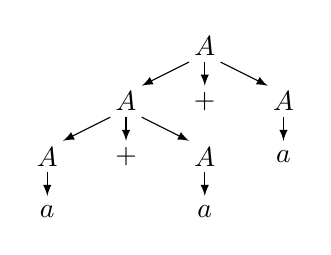
\begin{tikzpicture}
      \draw (5,7.1) node{$A$};
      \draw (4,6.4) node{$A$};
      \draw (5,6.4) node{$+$};
      \draw (6,6.4) node{$A$};
      \draw (3,5.7) node{$A$};
      \draw (4,5.7) node{$+$};
      \draw (5,5.7) node{$A$};
      \draw (3,5.0) node{$a$};
      \draw (6,5.7) node{$a$};
      \draw (5,5.0) node{$a$};

      \draw[-latex] (4.8,6.9) -- (4.2,6.6); 
      \draw[-latex] (5.0,6.9) -- (5.0,6.6); 
      \draw[-latex] (5.2,6.9) -- (5.8,6.6);
      
      \draw[-latex] (3.8,6.2) -- (3.2,5.9); 
      \draw[-latex] (4.0,6.2) -- (4.0,5.9); 
      \draw[-latex] (4.2,6.2) -- (4.8,5.9);
      
      \draw[-latex] (3.0,5.5) -- (3.0,5.2); 
      \draw[-latex] (5.0,5.5) -- (5.0,5.2); 
      \draw[-latex] (6.0,6.2) -- (6.0,5.9);
    \end{tikzpicture}}
    \hspace\fill
    \scalebox{.8}{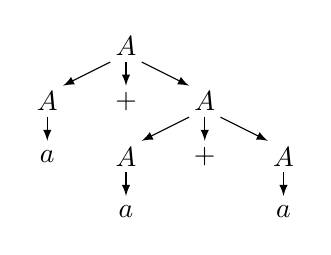
\begin{tikzpicture}
      \draw (5,7.1) node{$A$};
      \draw (4,6.4) node{$A$};
      \draw (5,6.4) node{$+$};
      \draw (6,6.4) node{$A$};
      \draw (5,5.7) node{$A$};
      \draw (6,5.7) node{$+$};
      \draw (7,5.7) node{$A$};

      \draw (4,5.7) node{$a$};
      \draw (5,5.0) node{$a$};
      \draw (7,5.0) node{$a$};

      \draw[-latex] (4.8,6.9) -- (4.2,6.6); 
      \draw[-latex] (5.0,6.9) -- (5.0,6.6); 
      \draw[-latex] (5.2,6.9) -- (5.8,6.6); 
      \draw[-latex] (5.8,6.2) -- (5.2,5.9); 
      \draw[-latex] (6.0,6.2) -- (6.0,5.9); 
      \draw[-latex] (6.2,6.2) -- (6.8,5.9); 
      \draw[-latex] (4.0,6.2) -- (4.0,5.9);
      \draw[-latex] (5.0,5.5) -- (5.0,5.2);
      \draw[-latex] (7.0,5.5) -- (7.0,5.2);
    \end{tikzpicture}}
    \hspace\fill
    \hspace\fill
  \end{exampleblock}

  \vspace{-2mm}
  \begin{block}{Théorème -- Indécidabilité de l'ambiguïté}
    Savoir si une grammaire $G$ est ambiguë est un problème indécidable.
  \end{block}
\end{frame}
\endgroup

% SPDX-License-Identifier: CC-BY-SA-4.0
% Author: Matthieu Perrin
% Part: <Nom de la partie>
% Section: <Nom de la section>
% Sub-section: <Nom de la sous-section>  % (facultatif, laisser vide si non utilisé)
% Frame: <Titre de la slide>

\begingroup

\begin{frame}{Démonstration de l'indécidabilité de l'ambiguïté}
  \small
  \begin{tikzpicture}
    \draw[white] (8, 3.6) -- (8, -1.5);

    \draw (8, 2.7) node{\begin{minipage}{\textwidth}
        Réduction du problème de correspondance de Post.
        \begin{itemize}
        \item Soit $\structure{D = \left\{d_1 = \HDomino{\alpha_1}{\beta_1}, ..., d_n = \HDomino{\alpha_n}{\beta_n} \right\}}$ une instance du PCP sur $\structure{\Sigma}$.
        \item<1,7->  $D$ a une solution ssi la grammaire $\alert{G_D}$ est ambigüe :

          \vspace{5mm}
          \uncover<7->{
            $$\begin{array}{rcl}
              G_D &=& \left\langle \Sigma \cup D, \{S, A, B\}, S, R \right\rangle
              \vspace{1mm}\\
              R &=& \left\{\begin{array}{rclclcl}
              S &\rightarrow& A \mid B\\
              A &\rightarrow& \alpha_1 \, A \, d_1 &\mid &...& \mid& \alpha_n \, A \, d_n \\
              A &\rightarrow& \alpha_1 \, \phantom{A\,} d_1 &\mid& ... &\mid& \alpha_n \,\phantom{A\,} d_n \\
              B &\rightarrow& \beta_1 \, B \, d_1 &\mid& ... &\mid& \beta_n \, B \, d_n \\
              B &\rightarrow& \beta_1 \, \phantom{B\,} d_1 &\mid& ... &\mid& \beta_n \, \phantom{B\,} d_n \\
              \end{array}\right.
            \end{array}
            $$
          }
          \vspace{5mm}

        \item<1,7-> Où la réduction $D \mapsto G_D$  est calculable.
        \item<1,7-> Or le problème de correspondance de Post est indécidable.
        \item<1,7-> Donc le problème de l'ambiguïté est indécidable. 
        \end{itemize}
    \end{minipage}};

    \draw<1> (8, 3) node{$G_D = ???$};

    
    \draw<2-5> (8, 2) node{\begin{minipage}{\textwidth}
        \begin{exampleblock}{Exemple pour $D = {\color{black}\left\{\HDomino[.7]{a}{baa}, \HDomino[.7]{ab}{aa}, \HDomino[.7]{bba}{bb} \right\}}$}

          \begin{enumerate}
          \item $D$ a pour solution $\footnotesize\HDomino{bba}{bb}\, \HDomino{ab}{aa}\, \HDomino{bba}{bb}\, \HDomino{a}{baa}$.
            \begin{itemize}
            \item<3-> On veut générer $bba ab bba a$ de deux manières différentes
              \begin{itemize}
              \item \structure{$S \vdash A\vdash^\star bba \cdot ab \cdot bba \cdot a$} et \example{$S \vdash B\vdash^\star bb \cdot aa \cdot bb \cdot baa$}
              \end{itemize}
            \end{itemize}
          \item<4-> $A$ et $B$ ne doivent pas engendrer $\varepsilon$
          \item<5-> $A$ et $B$ ne doivent pas être ambigües 
          \end{enumerate}

          \vspace{-4mm}
          $$G_D : \left\{\begin{array}{rcrcrcrcr}
          S &\rightarrow& \multicolumn{5}{l}{\uncover<3->{A \mid B}}\\
          \uncover<3->{A} &\uncover<3->{\rightarrow}&
          \uncover<3->{
            \structure{a}   \,A\, \uncover<5->{\footnotesize \HDomino{a}{baa}}  &\mid&
            \structure{ab}  \,A\, \uncover<5->{\footnotesize \HDomino{ab}{aa}}  &\mid&
            \structure{bba} \,A\, \uncover<5->{\footnotesize \HDomino{bba}{bb}} &\uncover<3>{\mid}&
            \uncover<3>{\varepsilon}
          }
          \\
          \uncover<4->{A} &\uncover<4->{\rightarrow}&
          \uncover<4->{
            \structure{a} \phantom{\,A\,} \uncover<5->{\footnotesize \HDomino{a}{baa}} &\mid&
            \structure{ab} \phantom{\,A\,} \uncover<5->{\footnotesize \HDomino{ab}{aa}} &\mid&
            \structure{bba} \phantom{\,A\,} \uncover<5->{\footnotesize \HDomino{bba}{bb}}
          }
          \\
          \uncover<3->{B} &\uncover<3->{\rightarrow}&
          \uncover<3->{
            \example{baa} \,B\, \uncover<5->{\footnotesize \HDomino{a}{baa}} &\mid&
            \example{aa} \,B\, \uncover<5->{\footnotesize \HDomino{ab}{aa}} &\mid&
            \example{bb} \,B\, \uncover<5->{\footnotesize \HDomino{bba}{bb}}&\uncover<3>{\mid}&
            \uncover<3>{\varepsilon}
          }
          \\
          \uncover<4->{B} &\uncover<4->{\rightarrow}&
          \uncover<4->{
            \example{baa} \phantom{\,B\,} \uncover<5->{\footnotesize \HDomino{a}{baa}} &\mid&
            \example{aa} \phantom{\,B\,} \uncover<5->{\footnotesize \HDomino{ab}{aa}} &\mid&
            \example{bb} \phantom{\,B\,} \uncover<5->{\footnotesize \HDomino{bba}{bb}}
          }
          \\
          \end{array}\right.$$
        \end{exampleblock}
    \end{minipage}};


    \draw<6> (8, 2.467) node{\begin{minipage}{\textwidth}
        \begin{exampleblock}{Exemple pour $D = {\color{black}\left\{\HDomino[.7]{a}{baa}, \HDomino[.7]{ab}{aa}, \HDomino[.7]{bba}{bb}\right\}}$}

          \vspace{-4mm}

          $$G_D : \left\{\begin{array}{rcrcrcrcr}
          S &\rightarrow& \multicolumn{5}{l}{\uncover<3->{A \mid B}}\\
          \uncover<3->{A} &\uncover<3->{\rightarrow}&
          \uncover<3->{
            \structure{a} \,A\, \uncover<5->{\footnotesize\HDomino{a}{baa}} &\mid&
            \structure{ab} \,A\, \uncover<5->{\footnotesize\HDomino{ab}{aa}} &\mid&
            \structure{bba} \,A\, \uncover<5->{\footnotesize\HDomino{bba}{bb}} &\uncover<3>{\mid}&
            \uncover<3>{\varepsilon}
          }
          \\
          \uncover<4->{A} &\uncover<4->{\rightarrow}&
          \uncover<4->{
            \structure{a} \phantom{\,A\,} \uncover<5->{\footnotesize\HDomino{a}{baa}} &\mid&
            \structure{ab} \phantom{\,A\,} \uncover<5->{\footnotesize\HDomino{ab}{aa}} &\mid&
            \structure{bba} \phantom{\,A\,} \uncover<5->{\footnotesize\HDomino{bba}{bb}}
          }
          \\
          \uncover<3->{B} &\uncover<3->{\rightarrow}&
          \uncover<3->{
            \example{baa} \,B\, \uncover<5->{\footnotesize\HDomino{a}{baa}} &\mid&
            \example{aa} \,B\, \uncover<5->{\footnotesize\HDomino{ab}{aa}} &\mid&
            \example{bb} \,B\, \uncover<5->{\footnotesize\HDomino{bba}{bb}}&\uncover<3>{\mid}&
            \uncover<3>{\varepsilon}
          }
          \\
          \uncover<4->{B} &\uncover<4->{\rightarrow}&
          \uncover<4->{
            \example{baa} \phantom{\,B\,} \uncover<5->{\footnotesize\HDomino{a}{baa}} &\mid&
            \example{aa} \phantom{\,B\,} \uncover<5->{\footnotesize\HDomino{ab}{aa}} &\mid&
            \example{bb} \phantom{\,B\,} \uncover<5->{\footnotesize\HDomino{bba}{bb}}
          }
          \\
          \end{array}\right.$$

          \begin{itemize}
          \item<6-> $G_D$ a deux dérivations pour : 
            $bbaabbbaa\, \scriptsize
            \HDomino{a}{baa}\, 
            \HDomino{bba}{bb}\,
            \HDomino{ab}{aa}\,
            \HDomino{bba}{bb}
            $.
            \begin{itemize}
            \item $S \vdash A \vdash^\star \structure{bba}\cdot \structure{ab} \cdot \structure{bba} \cdot \structure{a} \cdot \scriptsize
              \HDomino{a}{baa}\cdot
              \HDomino{bba}{bb}\cdot
              \HDomino{ab}{aa}\cdot
              \HDomino{bba}{bb}$
            \item $S \vdash B \vdash^\star \example{bb}\cdot \example{aa} \cdot \example{bb} \cdot \example{baa} \cdot\hspace{-.2mm} \scriptsize
              \HDomino{a}{baa}\cdot
              \HDomino{bba}{bb}\cdot
              \HDomino{ab}{aa}\cdot
              \HDomino{bba}{bb}$
            \end{itemize}
          \end{itemize}
        \end{exampleblock}
    \end{minipage}};
  \end{tikzpicture}
\end{frame}
\endgroup

 
 
\part{Complexité}
 
 
\section{Machines de Turing Non-Déterministes}
 
\subsection{Langages Générés et Engendrés}
% SPDX-License-Identifier: CC-BY-SA-4.0
% Author: Matthieu Perrin
% Part: 
% Section: 
% Sub-section: 
% Frame: 

\begingroup

\begin{frame}{Reconnaissance par une MTND}

  \onBlock[top=-4mm]{Définition -- Langage reconnu (ou accepté)}{
    Soient $M=\langle \Sigma, \Gamma, \blank, Q, q_0, F, \rightarrow \rangle$ une MTND et $L\subseteq \Sigma^\star$.
    \begin{itemize}
    \item On dit que \structure{$M$ reconnaît $L$} si \alert{$L = \mathcal{L}(M)$}
    \item \structure{Rappel :} $\mathcal{L}(M) \eqdef \left\{u \in \Sigma^\star \;\middle\mid\; \alert{\exists c \in \mathcal{C}_M^+, C_{\mathit{init}}(u) \leadsto_M^\star c} \right\}$
    \item On dit que \structure{$L$ est reconnaissable} s'il existe une MTND qui reconnaît $L$
    \item \structure{Rappel :} Si $M$ est déterministe, alors $\mathcal{L}(M)$ est semi-décidé par $M$
    \end{itemize}
  }

  \onExampleBlock[y=-2mm]{Exemple -- Reconnaissance de $\left\{u \cdot u \mid u \in \{a, b\}^\star \right\}$}{}

  \on[x=-25mm, y=-11mm]{
    \begin{tikzpicture}[tape, x=5mm, y=5mm]
      \node{\textsc{i}};
      \cell{}    
      \cell[structure on=<1>]{a} \smhead<1>
      \cell[structure ob=<2>]{b} \smheadb<2>
      \cell[structure ob=<3>]{a} \smheadb<3,4>
      \cell{b} \smheadb<6>  
      \cell{}  \smheadfromb<5>{-2}
    \end{tikzpicture}
  }

  \on[x=25mm, y=-11mm]{
    \begin{tikzpicture}[tape, x=5mm, y=5mm]
      \node{\textsc{u}};
      \cell{}                           \smheadfromb<4>{2}
      \cell[alert on=<1>]{\only<2->{a}} \smhead<1>
      \cell[alert ob=<2>]{\only<3->{b}} \smheadb<2,6>
      \cell[alert ob=<3>]{}             \smheadb<3>\smheadfromb<5>{-2}
      \cell{}    
      \cell{}  
    \end{tikzpicture}
  }

  \on[y=-30mm]{
    \begin{tikzpicture}[turingMachine,x=30mm]
      \state[initial, structure on=<1-3>] (0) at (0,0) {\faRandom};
      \state[structure ob=<4>]            (1) at (1,0) {\faFastBackward};
      \state[structure ob=<5>]            (2) at (2,0) {\faForward};
      \state[accepting, structure ob=<6>] (3) at (3,0) {\cmark};

      \path[structure on=<{1,3}>] (0) edge[loop above] node {\smGroup{\smTMtransR[\textsc{i}]{a}{a}\smTMtransR[\textsc{u}]{\alert<1,3>{\blank}}{a}}}   (0);
      \path[structure ob=<2>]     (0) edge[loop below] node {\smGroup{\smTMtransR[\textsc{i}]{b}{b}\smTMtransR[\textsc{u}]{\alertb<2>{\blank}}{b}}}    (0);
      \path[structure on=<1-3>]   (0) edge             node {\smTMtransL[\textsc{u}]{\alert<1-3>{\blank}}{\blank}}                                     (1);
      \path                       (1) edge[loop above] node {\smTMtransL[\textsc{u}]{a}{a}}                                                            (1);
      \path                       (1) edge[loop below] node {\smTMtransL[\textsc{u}]{b}{b}}                                                            (1);
      \path                       (1) edge             node {\smTMtransR[\textsc{u}]{\blank}{\blank}}                                                  (2);
      \path                       (2) edge[loop above] node {\smGroup{\smTMtransR[\textsc{i}]{a}{a}\smTMtransR[\textsc{u}]{a}{a}}}                     (2);
      \path                       (2) edge[loop below] node {\smGroup{\smTMtransR[\textsc{i}]{b}{b}\smTMtransR[\textsc{u}]{b}{b}}}                     (2);
      \path                       (2) edge             node {\smGroup{\smTMtransL[\textsc{i}]{\blank}{\blank}\smTMtransL[\textsc{u}]{\blank}{\blank}}} (3);
    \end{tikzpicture}
  }

\end{frame}

\endgroup



% SPDX-License-Identifier: CC-BY-SA-4.0
% Author: Matthieu Perrin
% Part: 
% Section: 
% Sub-section: 
% Frame: 

\begingroup

\begin{frame}{Exemples d'exécutions}
%    \item[\alert{$r$}] $\in \textsc{Ruban}_\Gamma$ : \structure{l'état de la bande}
%    La \structure{configuration initiale de $u$} est la configuration $\alert{C_{\mathit{init}}(u) \eqdef \langle \langle \varepsilon, u \rangle, q_0 \rangle}$.
  
  \onExampleBlock[y=1.2]{Exemples de mots}{
    \begin{itemize}
    \item Reconnaissance de \example{$ab$}
      \begin{itemize}
      \item $C_{\mathit{init}}(ab) = \langle \langle \varepsilon, ab \rangle, 0 \rangle \leadsto^\star \langle \langle ab, \varepsilon \rangle, 2 \rangle$
      \item $\langle \langle ab, \varepsilon \rangle, 2 \rangle$ est une configuration acceptante, donc \alert{$ab$ est reconnu}
      \end{itemize}
    \item<2-> Reconnaissance de \example{$ba$}
      \begin{itemize}
      \item $C_{\mathit{init}}(ba) = \alert<2>{\langle \langle \varepsilon, ba \rangle, 0 \rangle}$
      \item $\langle \langle \varepsilon, ba \rangle, 0 \rangle$ est une configuration d'arrêt donc \alert{$ba$ n'est pas reconnu}
      \end{itemize}
    \item<3-> Reconnaissance de \example{$aa$}
      \begin{itemize}
      \item $C_{\mathit{init}}(aa) = \alert<3>{\langle \langle \varepsilon, aa \rangle, 0 \rangle}
        \only<4->{\leadsto \alert<4>{\langle \langle a, a \rangle, 1 \rangle}}
        \only<5->{\leadsto \alert<5>{\langle \langle \varepsilon, aa \rangle, 0 \rangle} \leadsto \ldots}$
      \item<6-> Mais aussi $C_{\mathit{init}}(aa) \leadsto^\star \langle \langle ab, \varepsilon \rangle, 2 \rangle$, donc \alert{$aa$ est reconnu}
      \end{itemize}
    \end{itemize}
  }
  
  \onBlock[y=-1.8]{Représentation des configurations}{}
  
  \on[x=-2.9,y=-3] {
    \begin{tikzpicture}[tape, x=7mm, y=7mm]
      \cell{$\blank $}
      \cell{\alt<2>{$b$}{$a$}}   \smhead[ob=<{2,3,5}>]
      \cell{\alt<2-5>{$a$}{$b$}} \smhead[ob=<{4}>]
      \cell{$\blank $}                \smhead[ob=<{1,6-}>]
    \end{tikzpicture}
  }

  \on[x=2.9,y=-2.9] {
    \begin{tikzpicture}[turingMachine]
      \state[alert ob=<{2,3,5}>, initial  ] (0) at (0,0) {0}; 
      \state[alert ob=<{4}>               ] (1) at (1,0) {1}; 
      \state[alert ob=<{1,6-}>,  accepting] (2) at (2,0) {2}; 
      
      \path (0) edge[bend left] node {\smTMtransR{a}{a}} (1);
      \path (1) edge[bend left] node {\smTMtransL{a}{a}} (0);
      \path (1) edge            node {\smAlign{\smTMtransR{a}{b}\smTMtransR{b}{b}}} (2);
    \end{tikzpicture}
  }
  
\end{frame}

\endgroup

 
% SPDX-License-Identifier: CC-BY-SA-4.0
% Author: Matthieu Perrin
% Part: 
% Section: 
% Sub-section: 
% Frame: 

\begingroup

\begin{frame}{Générateur d'un langage}
  
  \onBlock[top=-2mm]{Langage généré par $M$}{
    Soit $M=\langle \Sigma, \Gamma, \blank, Q, q_0, F, \rightarrow \rangle$ une machine de Turing. 
 
    Le langage \structure{généré} par $M$ est l'ensemble $\alert{\mathcal{L}_G(M)}$ des mots écrits sur le ruban quand $M$ atteint un état accepteur à partir de $C_{\mathit{init}}(\varepsilon)$ :
    $$
    \alert{\mathcal{L}_G(M) \eqdef \left\{ \mathit{mot}(r) \in \Sigma^\star \middle| \exists q_f\in F, C_{\mathit{init}}(\varepsilon) \leadsto_M^\star \langle r, q_f \rangle \right\}}.
    $$
 
    \begin{itemize}
    \item $\langle r, q_f \rangle$ n'est pas forcément une configuration d'arrêt
    \item $M$ est appelée un \structure{générateur} du langage $\mathcal{L}_G(M)$
    \end{itemize}
  }
  
  \onExampleBlock[y=-15mm]{Exemple : générateur du langage $\mathcal{L}(ba^\star b)$}{}
 
  \on[y=-30mm, x=-30mm]{
    \begin{tikzpicture}[tape, x=7mm, y=7mm]
      \cell{$\blank$}
      \cell{\alt<-1>{$\blank$}{$b$}} \smheadb<1>  
      \cell{\alt<-2>{$\blank$}{$a$}} \smheadb<2> 
      \cell{\alt<-2>{$\blank$}{$a$}} 
      \cell{\alt<-3>{$\blank$}{$b$}} \smheadfromb<3>{-2}
      \cell{$\blank$}                \smheadb<4> 
    \end{tikzpicture}
  }
  
  \on[y=-30mm, x=30mm]{
    \begin{tikzpicture}[turingMachine]
      \state[alert on=<{1}>,   initial] (0) at (0,0) {$0$}; 
      \state[alert ob=<{2,3}>         ] (1) at (1,0) {$1$}; 
      \state[alert ob=<{4}>, accepting] (2) at (2,0) {$2$}; 
      
      \path (0) edge             node {\smTMtransR{\blank}{b}} (1);
      \path (1) edge[loop below] node {\smTMtransR{\blank}{a}} (1);
      \path (1) edge             node {\smTMtransR{\blank}{b}} (2);
    \end{tikzpicture}
  }

\end{frame}

\endgroup

% SPDX-License-Identifier: CC-BY-SA-4.0
% Author: Matthieu Perrin
% Part: 
% Section: 
% Sub-section: 
% Frame: 

\begingroup

\begin{frame}{Équivalence entre automates à pile et grammaires}

  \onBlock[top=-2mm, left=.6\textwidth]{Théorème de Chomsky et Schützenberger}{
    Un langage est \structure{algébrique} si et seulement s’il est reconnu par un \structure{automate à pile non déterministe}.
  }

  \onImage[top, x=.35\textwidth]{%
    height=25mm,
    title={Marcel-Paul Schützenberger},
    licenselogo={\ccby},
    license={{\href{https://creativecommons.org/licenses/by/2.0/}{CC BY-2.0}} -- Konrad Jacobs, 1972 (\href{https://commons.wikimedia.org/wiki/File:Sch\%C3\%BCtzenberger.jpeg?uselang=fr}{Wikimedia})},
    img={Schutzenberger.jpeg}
  }

 \onExampleBlock<2->[y=0mm]{Exemple : $\{ a^n c b^n \mid n\in \mathbb{N} \}$}{}
 
 \on<2->[bottom=9mm,x=-.45\textwidth]{
   \begin{tikzpicture}[stack, x=7mm, y=7mm]
     \cell[alert ob=<2>]{\oneof[$S$]{\on<3->{$T$}\on<5->{$B$}\on<7->{}}}
     \cell              {\oneof[]{\on<3>{$A$}\on<5>{$S$}}}
   \end{tikzpicture}
 }
 
 \on<2->[bottom=23mm,x=-.3\textwidth]{
   \begin{tikzpicture}[word, x=5mm, y=5mm]
     \cell[alert ob=<4->]{$a$} \smhead[on=<-3>]
     \cell[alert ob=<6->]{$c$} \smhead[ob=<4-5>]
     \cell[alert ob=<7->]{$b$} \smhead[ob=<6>]
   \end{tikzpicture}
 }
 
 \on<2->[bottom=10mm,x=-.15\textwidth]{\small
   \begin{tikzpicture}[pushdown]
     \state[initial above, accepting, initial text={\alertb<2>{$S$}}] (q) {};
     \path (q) edge [loop left] node {
       $\begin{array}{r}
         \alertb<4>{\smPAtrans{a}{A}{\varepsilon}} \\
         \alertb<7>{\smPAtrans{b}{B}{\varepsilon}} \\
         \alertb<6>{\smPAtrans{c}{S}{\varepsilon}} \\
       \end{array}$
     } (q);
     \path (q) edge [loop right] node {
       $\begin{array}{l}
         \alertb<3>{\smPAtrans{\varepsilon}{S}{TA}} \\
         \alertb<5>{\smPAtrans{\varepsilon}{T}{BS}} \\
       \end{array}$
     } (q);
   \end{tikzpicture}
 }
 
 \on<2->[bottom=15mm, x=.2\textwidth, width=2.5cm]{
   \example{Grammaire}\\\vspace{2mm}
   $\left\{\begin{array}{@{\,}r@{~\rightarrow~}l@{\,}}
   S & \alertb<3>{AT} \mid \alertb<6>{c}\\
   T & \alertb<5>{SB}\\
   A & \alertb<4>{a}\\
   B & \alertb<7>{b}\\
   \end{array}\right.$
 }
 
 \on<2->[bottom=10mm,x=.4\textwidth]{
   \begin{tikzpicture}[tree, x=7mm,y=7mm, tree node internal/.append style={structure,}, tree node leave/.append style={example,},]
     \tree{\alertb<2>{$S$}}{
       \tree[on=<3->]{\alertb<3>{$A$}}{
         \tree[on=<4->,yshift=-1]{\alertb<4>{$a$}}{}
       }
       \tree[on=<3->]{\alertb<3>{$T$}}{
         \tree[on=<5->]{\alertb<5>{$S$}}{
           \tree[on=<6->]{\alertb<6>{$c$}}{}
         }
         \tree[on=<5->]{\alertb<5>{$B$}}{
           \tree[on=<7->]{\alertb<7>{$b$}}{}
         }
       }
     }
   \end{tikzpicture}
 }

  \footnoteref{Chomsky, Schützenberger. \emph{The algebraic theory of context-free languages.} SLFM. (1959)}
  
\end{frame}

\endgroup

% SPDX-License-Identifier: CC-BY-SA-4.0
% Author: Matthieu Perrin
% Part: 
% Section: 
% Sub-section: 
% Frame: 

\begingroup

\SetKwFunction{Ecrire}{ecrire}
\SetKwFunction{Reconnait}{reconnait}
\SetKwFunction{Generer}{generer}

\begin{frame}{$1 \Rightarrow 2$}

  \onBlock[top=-2mm]{Lemme -- Reconnu $\Rightarrow$ généré}{
    Soit $L$ un langage reconnaissable par une MTND $M$.\\
    Alors il existe une MTND $M_G$ qui génère $L$.
  }

  \onBlock[y=2mm]{Démonstration}{
    On construit un générateur $M_G$ de $L$ :
    \begin{itemize}
    \item Générer tous les mots de $\Sigma^\star$ sur deux rubans $r$ et $g$
    \item \alert{De manière non-déterministe}, tenter de reconnaître chaque mot sur $r$
    \item Si le mot est reconnu, il est toujours écrit sur $g$
    \end{itemize}
  }

  \on[left=.5\textwidth, y=-30mm]{
    \begin{algorithm}[H]
      \Algo{$\Generer_L$}{
        \For{$u \in \Sigma^\star$}{
          \If{$\Reconnait_L(u)$} {
            $\Ecrire (u)$\;
          }
        }
      }
    \end{algorithm}
  }

  \on[right=.5\textwidth, y=-25mm]{
    \begin{tikzpicture}[turingMachine]
      \state[initial]              (A)  at (0,0) {$\Sigma^\star$};
      \state[structure]            (M0) at (1,0) {$M_0$};
      \state[accepting, structure] (Mf) at (2,0) {$M_f$};
      \cloudPath[structure] {M0}{Mf}
      \path (A) edge[loop above] node       {\smGroup{\smTMtransL[r]{\blank}{x}\smTMtransL[g]{\blank}{x}} $\forall x \in \Sigma$} (A);
      \path (A) edge             node[swap] {\smGroup{\smTMtransR[r]{\blank}{\blank}\smTMtransR[g]{\blank}{\blank}}} (M0);
    \end{tikzpicture}
  }
  
\end{frame}

\endgroup

% SPDX-License-Identifier: CC-BY-SA-4.0
% Author: Matthieu Perrin
% Part: 
% Section: 
% Sub-section: 
% Frame: 

\begingroup

\begin{frame}{Exemples : génération de $\{a^n b^n \mid n\in \mathbb{N}\}$}

  \on[top]{%
    \begin{tikzpicture}[tape, x=7mm, y=7mm]
      \node[left]{$r :$};
      \cell{$\blank$}
      \cell{$\blank$} 
      \cell{$\blank$}                         \smheadb<5> 
      \cell{\oneof[$\blank$]{\on<5-6>{$a$}}}  \smheadb<4,6>     \smheadfromb<9>{2}
      \cell{\oneof[$\blank$]{\on<4-10>{$a$}}} \smheadb<3,10,13>
      \cell{\oneof[$\blank$]{\on<3-12>{$b$}}} \smheadb<2,12,14> 
      \cell{\oneof[$\blank$]{\on<2-8>{$b$}}}  \smhead <1,8,15>  \smheadfromb<11>{-1}
      \cell{$\blank$}                                           \smheadfromb<7>{-3}
      \cell{$\blank$}
      \cell{$\blank$}
    \end{tikzpicture}
  }

  \on[y=13mm]{%
    \begin{tikzpicture}[tape, x=7mm, y=7mm]
      \node[left]{$g :$};
      \cell{$\blank$}
      \cell{$\blank$} 
      \cell{$\blank$}                       \smheadb<5> 
      \cell{\oneof[$\blank$]{\on<5->{$a$}}} \smheadb<4,6-> 
      \cell{\oneof[$\blank$]{\on<4->{$a$}}} \smheadb<3> 
      \cell{\oneof[$\blank$]{\on<3->{$b$}}} \smheadb<2> 
      \cell{\oneof[$\blank$]{\on<2->{$b$}}} \smhead <1> 
      \cell{$\blank$}
      \cell{$\blank$}
      \cell{$\blank$}
    \end{tikzpicture}
  }

  \on[bottom]{%
    \begin{tikzpicture}[turingMachine, x=15mm, y=15mm]
      \state[         , alert ob=<{-5}>,      initial above] (S) at (0,2) {$\Sigma^\star$}; 
      \state[structure, alert ob=<{6,10,14}>,              ] (0) at (2,2) {$\textbf{A}$}; 
      \state[structure, alert ob=<{7,11}>,                 ] (1) at (1,1) {\faForward}; 
      \state[structure, alert ob=<{8,12}>,                 ] (2) at (2,0) {$\textbf{B}$}; 
      \state[structure, alert ob=<{9,13}>,                 ] (3) at (3,1) {\faBackward}; 
      \state[structure, alert ob=<{15}>,      accepting    ] (f) at (4,2) {\faCheck}; 

      \scriptsize
      \path (S) edge[loop left]  node       {$\begin{array}{r}\smGroup{\smTMtransL[r]{\blank}{a}\smTMtransL[g]{\blank}{a}}\\\smGroup{\smTMtransL[r]{\blank}{b}\smTMtransL[g]{\blank}{b}}\end{array}$} (S);
      \path (1) edge[loop left]  node       {\smAlign{\smTMtransR[r]{a}{a}\smTMtransR[r]{b}{b}}} (1);
      \path (3) edge[loop right] node       {\smAlign{\smTMtransL[r]{a}{a}\smTMtransL[r]{b}{b}}} (3);
      \path (S) edge             node       {\smGroup{\smTMtransR[r]{\blank}{\blank}\smTMtransR[g]{\blank}{\blank}}} (0);
      \path (0) edge             node       {\smTMtransR[r]{\blank}{\blank}} (f);
      \path (0) edge             node[swap] {\smTMtransR[r]{a} {\blank}} (1);
      \path (1) edge             node[swap] {\smTMtransL[r]{\blank}{\blank}} (2);
      \path (2) edge             node[swap] {\smTMtransL[r]{b} {\blank}} (3);
      \path (3) edge             node[swap] {\smTMtransR[r]{\blank}{\blank}} (0);
    \end{tikzpicture}
  }

\end{frame}

\endgroup

% SPDX-License-Identifier: CC-BY-SA-4.0
% Author: Matthieu Perrin
% Part: 
% Section: 
% Sub-section: 
% Frame: 

\begingroup

\begin{frame}{$2 \Rightarrow 3$}

  \begin{block}{Lemme -- Généré $\Rightarrow$ engendré}
    Soit $L$ un langage généré par une MTND $M_G$.\\
    Alors il existe une grammaire $G$ qui engendre $L$. 
  \end{block}

  \vfill

  \begin{block}{Démonstration}
    Soit $\structure{M_G = \langle \Sigma, \Gamma, \blank, Q, q_0, F, \rightarrow \rangle}$ un générateur de $L$.\\
    $L$ est engendré par la grammaire $\alert{G = \langle \Sigma, \Gamma \setminus \Sigma \cup Q \cup \{S, G, D\}, S, R \rangle}$, avec

    \vspace{-4mm}
    $$\alert{R = \left\{ \begin{array}{rclcl}
        S & \rightarrow & G q_0 D  \\
        G &\rightarrow& G\blank \mid \varepsilon  &,&   G\blank \,\,\rightarrow\,\, G\\
        D &\rightarrow& \blank D \mid \varepsilon &,&   \blank D \,\,\rightarrow\,\, D \\
        \\
        q a & \rightarrow & a' q' & : & q \xrightarrow{\smTMtransR{a}{a'}} q' \in \rightarrow \\
        b q a & \rightarrow & q' b a' & : & q \xrightarrow{\smTMtransL{a}{a'}} q' \in \rightarrow, b\in \Gamma \\
        \\
        q_f & \rightarrow & \varepsilon & : & q_f \in F \\
      \end{array}\right\}}$$
  \end{block}

\end{frame}

\endgroup

% SPDX-License-Identifier: CC-BY-SA-4.0
% Author: Matthieu Perrin
% Part: 
% Section: 
% Sub-section: 
% Frame: 

\begingroup

\begin{frame}{Exemple : le langage $\mathcal{L}(ba^\star b)$}

  \on[y=20mm, x=20mm]{
    \begin{tikzpicture}[tape, x=7mm, y=7mm]
      \cell{$\blank$}                
      \cell{\alt<-3>{$\blank$}{$b$}} \smheadb<3>
      \cell{\alt<-4>{$\blank$}{$a$}} \smheadb<4,6>
      \cell{\alt<-5>{$\blank$}{$b$}} \smheadb<5>
      \cell{$\blank$}                 
    \end{tikzpicture}
  }

  \on[y=0mm, x=20mm]{
    \begin{tikzpicture}[turingMachine]
      \state [alert on=<{-3}>,  initial  ] (0) at (0,0) {$0$}; 
      \state [alert on=<{4,5}>,          ] (1) at (1,0) {$1$}; 
      \state [alert on=<{6-}>,  accepting] (2) at (2,0) {$2$}; 

      \path (0) edge             node {$\smTMtransR{\blank}{b}$} (1);
      \path (1) edge[loop below] node {$\smTMtransR{\blank}{a}$} (1);
      \path (1) edge             node {$\smTMtransL{\blank}{b}$} (2);
    \end{tikzpicture}
  }

  \on[left=40mm]{
    $G = \left\{\begin{array}{rcl}
      \alertb<2>{S}      & \alertb<2>{\rightarrow} & \alertb<2>{G 0 D}                             \\
      \alertb<7>{G}      & \alertb<7>{\rightarrow} & G\blank \mid \alertb<7>{\varepsilon}              \\
      G\blank                &\rightarrow              & G                                             \\
      \alertb<3,7>{D}    &\alertb<3,7>{\rightarrow}& \alertb<3>{\blank D} \mid \alertb<7>{\varepsilon} \\
      \blank D               &\rightarrow              & D                                             \\
      \\                                                                                        
      \alertb<4>{0 \blank}   & \alertb<4>{\rightarrow} & \alertb<4>{b 1}                               \\
      \alertb<5>{1 \blank}   & \alertb<5>{\rightarrow} & \alertb<5>{a 1}                               \\
      \alertb<6>{a 1 \blank} & \alertb<6>{\rightarrow} & \alertb<6>{2 a b}                             \\
      b 1 \blank             & \rightarrow             & 2 b b                                         \\
      \blank 1 \blank            & \rightarrow             & 2 \blank b                                        \\
      \\                                                                                         
      \alertb<7>{2}      & \alertb<7>{\rightarrow} & \alertb<7>{\varepsilon}                       \\
    \end{array}\right.$
  }

  \on[y=-25mm, x=20mm]{
    $\begin{array}{r@{~~}l@{~~}l@{~~}l@{~~}l} 
      S & \uncover<2->{\vdash\phantom{^\star}} & \uncover<2->{G \structure{\alertb<2>{0}} D}                                                                                      \\
      &   \uncover<3->{\vdash^\star}           & \uncover<3->{G 0 \structure{\alertb<3>{\blank}} D}\phantom{DD} & \uncover<4->{\vdash} & \uncover<4->{G \structure{b \alertb<4>{1}} D}      \\
      &   \uncover<5->{\vdash^\star}           & \uncover<5->{G b 1 \structure{\blank} D}                       & \uncover<5->{\vdash} & \uncover<5->{G b \structure{\alertb<5>{a 1}} D}    \\
      &   \uncover<6->{\vdash^\star}           & \uncover<6->{G b a 1 \structure{\blank} D}                     & \uncover<6->{\vdash} & \uncover<6->{G b \structure{\alertb<5>{2 a b}} D}  \\
      &   \uncover<7->{\vdash^\star}           & \uncover<7->{b a b}                                                                                                              \\
    \end{array}$
  }

\end{frame}

\endgroup

% SPDX-License-Identifier: CC-BY-SA-4.0
% Author: Matthieu Perrin
% Part: 
% Section: 
% Sub-section: 
% Frame: 

\begingroup

\begin{frame}{$3 \Rightarrow 1$}

  \begin{block}{Lemme -- Généré $\Rightarrow$ reconnu}
    Soit $L$ un langage engendré par une grammaire $G$.\\
    Alors il existe une une MTND $M$ qui reconnaît $L$. 
  \end{block}
  
  \begin{block}{Démonstration}
    \begin{itemize}
    \item Rappel : Algorithme de recherche ascendante par force brute
      \begin{description}
      \item [Entrées :]
        \begin{itemize}
        \item Une grammaire $G$, si possible contextuelle
        \item Un mot $u$
        \end{itemize}
      \item [Sortie :] une réponse booléenne sur \structure{$u \in \mathcal{L}(G)$}
      \item [Teminaison :] garantie si $G$ est contextuelle
      \end{description}
    \item Le non-déterminisme permet de simplifier l'algorithme
    \end{itemize}
  \end{block}

\end{frame}

\endgroup

% SPDX-License-Identifier: CC-BY-SA-4.0
% Author: Matthieu Perrin
% Part: 
% Section: 
% Sub-section: 
% Frame: 

\begingroup

\SetKwFunction{Forcebrute}{force\_brute}
\SetKwData{Old}{old}
\SetKwData{New}{etape}
\SetKwData{Vu}{explore}

\begin{frame}[fragile]{Recherche ascendante par force brute}

  \on[top=-2mm]{
    \begin{algorithm}[H]
      \Fun{$\Forcebrute(G = \langle \Sigma, \Gamma, S, R \rangle \text{: grammaire}, u \in \Sigma^\star) \in \mathbb{B}$}{
        \Alertb<1>{$\New \leftarrow \{u\}$};
        $\Vu \leftarrow \New$;\\
        \While{$\Alertb<5>{\New \neq \emptyset} \land \Alertb<4-5>{S\notin \New}$}{
          \Alertb<2-3>{$\New \leftarrow \{ v\in (\Sigma \cup \Gamma)^\star \,|\, \exists w \in \New, v \vdash w \} \setminus \Vu$};\\
          $\Vu \leftarrow \Vu \cup \New$;\\
        }
        \Return \Alertb<4>{$S \in \New$};\\
      }
    \end{algorithm}
  }

  \onExampleBlock[y=-2mm]{$abc \in L$}{
    $\begin{array}{@{}l@{~~~~}l@{~~}l@{~~}l@{~~}l@{~~}l@{~~}l@{}}
      \alert<1>{\{\alertb<2>{ab}\structureb<2>{c}\}}
      \uncover<2->{&\leftarrow & \{\alertb<2>{aB}\structureb<3>{c}, \alertb<3>{ab}\structureb<2>{C}\}}
      \uncover<3->{&\leftarrow& \{\alertb<3>{aB}\structureb<3>{C}\}} \\
      \uncover<4->{& \leftarrow & \{aBX\} &
        \leftarrow & \{aCX\} &
        \leftarrow & \{aCB\} \\
        & \leftarrow & \{\alert<4>{S}\} \\}
    \end{array}$
  }

  \onExampleBlock<5->[bottom]{$abbc \notin L$}{
    $\begin{array}{@{}l@{~~}c@{~~}l@{~~}c@{~~}l@{}}
      \alert{\{abbc\}} & \leftarrow & \{aBbc, abBc, abbC\} & \leftarrow & \{aBBc, aBbC, abBC\} \\
      & \leftarrow & \{aBBC, abBX\} & \leftarrow & \{aBBX, abCX\} \\
      & \leftarrow & \{aBCX, abCB\} & \leftarrow & \{aBXX, aBCB\} \\
      & \leftarrow & \{aCXX, aBXB\} & \leftarrow & \{aCBX, aCXB\} \\
      & \leftarrow & \{aCCX, aCBB\} & \leftarrow & \{aCCB, aCBB\} \\
      & \leftarrow & \alert{\emptyset} \\
    \end{array}$
  }

  \on[x=35mm]{
    \example{$
      \left\{\begin{array}{rcl}
      S   & \rightarrow & aCB  \\
      C B & \rightarrow & C X  \\
      C X & \rightarrow & B X  \\
      B X & \rightarrow & B C  \\
      \alertb<2,3>{a B} & \alertb<2,3>{\rightarrow} & \alertb<2,3>{a b}  \\
      b B & \rightarrow & b b  \\
      \structureb<2,3>{C}   & \structureb<2,3>{\rightarrow} & \structureb<2,3>{c}
      \end{array}\right.
      $}
  }
  
\end{frame}

\endgroup

% SPDX-License-Identifier: CC-BY-SA-4.0
% Author: Matthieu Perrin
% Part: 
% Section: 
% Sub-section: 
% Frame: 

\begingroup

\SetKwFunction{Enumere}{enumere}
\SetKwFunction{Reconnait}{reconnait}
\SetKwFunction{Generer}{generer}

\begin{frame}{Tout langage engendré est reconnaissable}

  \on[text, y=-3mm]{
    Soit $L$ un langage engendré par une grammaire $G = \langle \Sigma, \Gamma, S, R \rangle$.\\
    
    Alors $L$ est reconnu par la machine $M$ suivant l'algorithme de \\
    \structure{recherche ascendante par force brute} \alert{non-déterministe} suivant : 

    \begin{algorithm}[H]\small
      \Fun{$\Reconnait_L(u)$}{
        \While{$u \neq S$}{
          \tcp{}
          \tcp{}
          \tcp{}
          Choisir une règle $\structure{g \rightarrow d \in R}$ de manière \alert{non-déterministe}\;
          \tcp{}
          \tcp{}
          \tcp{}
          \tcp{}
          Déplacer la tête de lecture à $\structure{\langle G, D\rangle}$ de manière \alert{non-déterministe}\;
          \tcp{}
          \tcp{}
          \tcp{}
          \leIf{$\exists D' : D=d D'$}{$u \leftarrow G g D'$}{bloquer}
          \tcp{}
          \tcp{}
          \tcp{}
        }
        \Return \True\;
      }
    \end{algorithm}
  }
  
  \on<2->[x=-42mm, y=12mm, anchor=west]{\small
    \begin{tikzpicture}[turingMachine,x=15mm]
      \state[initial  ] (q0) at (0,0) {$q_0$};
      \state[         ] (5b) at (1,0) {};
      \state[         ] (5c) at (2,0) {};
      \state[accepting] (5d) at (3,0) {};
      
      \path[densely dotted] (q0) edge[loop above]                              (q0);
      \path                 (q0) edge             node {$\smTMtransR{\blank}{\blank}$} (5b);
      \path                 (5b) edge             node {$\smTMtransR{S}{S}$}   (5c);
      \path                 (5c) edge             node {$\smTMtransL{\blank}{\blank}$} (5d);
    \end{tikzpicture}
  }
  
  \on<3->[x=-42mm, y=-2mm, anchor=west]{\small
    \begin{tikzpicture}[turingMachine]
      \state[initial] (q0) {$q_0$};
      \draw[-latex] (q0.east) -- +(5mm,2mm ) node[right]{$r_1$};
      \draw[-latex] (q0.east) -- +(5mm,0   ) node[right]{$r_2$};
      \draw[-latex] (q0.east) -- +(5mm,-2mm) node[right]{$r_3$};
    \end{tikzpicture}
  }

  \on<4->[x=-42mm, y=-16mm, anchor=west]{\small
    \begin{tikzpicture}[turingMachine]
      \state[initial] (q0) {$q_0$};
      \path (q0) edge[loop right] node{\smGroup{\smTMtransL{\star}{\star}\smTMtransR{\star}{\star}}} (q0);
    \end{tikzpicture}
  }

  \on<5->[x=-42mm, y=-29mm, anchor=west]{
    \begin{tikzpicture}[turingMachine, x=15mm]\small
      \state[initial] (q0) at (0,0) {$q_0$};
      \state          (2b) at (1,0) {};
      \state          (2c) at (2,0) {};
      \state          (2d) at (3,0) {};
      \state          (2e) at (4,0) {};
      \state          (2f) at (5,0) {};
      \state          (q1) at (6,0) {$q_0$};

      \draw (q0) edge node {\smTMtransM{d_1}}          (2b);
      \path (2b) edge node {\smTMtransM{...}}          (2c);
      \path (2c) edge node {\smTMtransM{d_{|d|}}}       (2d);
      \path (2d) edge node {\smTMtransP{\star}{g_1}}    (2e);
      \draw (2e) edge node {\smTMtransP{\star}{...}}    (2f);
      \draw (2f) edge node {\smTMtransP{\star}{g_{|g|}}} (q1);
    \end{tikzpicture}
  }

\end{frame}

\endgroup

% SPDX-License-Identifier: CC-BY-SA-4.0
% Author: Matthieu Perrin
% Part: 
% Section: 
% Sub-section: 
% Frame: 

\begingroup

\begin{frame}{Exemple : le langage $\{a^n b^n c^n \mid n>0\}$}

  \on[top]{
    \example{
      $aabbcc\uncover<9->{\leftarrow aabBcc}\uncover<11->{\leftarrow aabcBc}\uncover<13->{\leftarrow aSBc}\uncover<15->{\leftarrow S}$
    }
  }

  \ob<4> [y=15mm]{\alert{Bloqué !}}
  \ob<16>[y=15mm]{\alert{Mot reconnu !}}

  \on[top=5mm]{   
    \begin{tikzpicture}[tape, x=7mm, y=7mm]
      \cell{$\blank$}                                                               
      \cell{\oneof[$a$]{\on<15->{$S$}}}                                       \smhead<1,14>  
      \cell{\oneof[$a$]{\on<3-4>{$b$}\on<13-14>{$S$}\on<15->{$\blank$}}}          \smheadb<3-4,12,15,16>  \smheadfromb<2>{-1}\smheadfromb<15>{-1}\smheadfromb<16>{-2}
      \cell{\oneof[$b$]{\on<4,7>{$c$}\on<13-14>{$B$}\on<15->{$\blank$}}}          \smheadb<6-7,13>        \smheadfromb<5>{-2}\smheadfromb<13>{-1}
      \cell{\oneof[$b$]{\on<3-4,6-8,11-14>{$c$}\on<9,10>{$B$}\on<15->{$\blank$}}} \smheadb<8,10>   
      \cell{\oneof[$c$]{\on<4,7,13->{$\blank$}\on<11-12>{$B$}}}                   \smheadb<9>             \smheadfromb<11>{-1}
      \cell{\oneof[$c$]{\on<3-4,6-8,13->{$\blank$}}}                              
      \cell{$\blank$}                                                             
    \end{tikzpicture}
  }

  \on[bottom]{
    \begin{tikzpicture}[turingMachine,x=15mm, y=9mm]
      \path[anchor=mid,example] (-1cm,3) node [left=1mm]{$S $} node (G1) {$\rightarrow$} node[right=1mm]{$abc$} ;
      \path[anchor=mid,example] (-1cm,2) node [left=1mm]{$S $} node (G2) {$\rightarrow$} node[right=1mm]{$aSBc$};
      \path[anchor=mid,example] (-1cm,1) node [left=1mm]{$cB$} node (G3) {$\rightarrow$} node[right=1mm]{$Bc$}  ;
      \path[anchor=mid,example] (-1cm,0) node [left=1mm]{$bB$} node (G4) {$\rightarrow$} node[right=1mm]{$bb$}  ;
      \draw[example, decorate, decoration={brace, amplitude=10pt, raise=3mm}] (G4.south west) -- (G1.north west);

      \node                                             (q1) at (5,4) {}; 
      \state[alert ob=<{1,2,5,9,10,12,14,16}>, initial] (q0) at (0,4) {$q_0$};
      \state[alert ob=<{3,13}>                        ] (1b) at (1,3) {};
      \state[alert ob=<{4,13}>                        ] (1c) at (2,3) {};
      \state[alert ob=<13>                            ] (1d) at (3,3) {};
      \state[alert ob=<15>                            ] (2b) at (1,2) {};
      \state[alert ob=<15>                            ] (2c) at (2,2) {};
      \state[alert ob=<15>                            ] (2d) at (3,2) {};
      \state[alert ob=<15>                            ] (2e) at (4,2) {};
      \state[alert ob=<11>                            ] (3b) at (1,1) {};
      \state[alert ob=<11>                            ] (3c) at (2,1) {};
      \state[alert ob=<11>                            ] (3d) at (3,1) {};
      \state[alert ob=<6>                             ] (4b) at (1,0) {};
      \state[alert ob=<7>                             ] (4c) at (2,0) {};
      \state[alert ob=<8>                             ] (4d) at (3,0) {};
      \state[alert ob=<16>                            ] (5b) at (1,5) {};
      \state[alert ob=<16>                            ] (5c) at (2,5) {};
      \state[alert ob=<16>,                  accepting] (5d) at (3,5) {};

      \path (q0) edge[loop, out=120, in=150] node[above left] {\smGroup{\smTMtransL{x}{x}\smTMtransR{x}{x}}} (q0);
      \path (1b) edge                        node             {\smTMtransM{b}}                               (1c);
      \path (1c) edge                        node             {\smTMtransM{c}}                               (1d);
      \path (2b) edge                        node             {\smTMtransM{S}}                               (2c);
      \path (2c) edge                        node             {\smTMtransM{B}}                               (2d);
      \path (2d) edge                        node             {\smTMtransM{c}}                               (2e);
      \path (3b) edge                        node             {\smTMtransM{c}}                               (3c);
      \path (3c) edge                        node             {\smTMtransP{x}{c}}                            (3d);
      \path (4b) edge                        node             {\smTMtransM{b}}                               (4c);
      \path (4c) edge                        node             {\smTMtransP{x}{b}}                            (4d);
      \path (5b) edge                        node             {\smTMtransR{S}{S}}                            (5c);
      \path (5c) edge                        node             {\smTMtransL{\blank}{\blank}}                          (5d);

      \draw [-latex, rounded corners] (q0) -- (0,3) -- node {\smTMtransM{a}}        (1b);
      \draw [-latex, rounded corners] (q0) -- (0,2) -- node {\smTMtransM{a}}        (2b);
      \draw [-latex, rounded corners] (q0) -- (0,1) -- node {\smTMtransM{B}}        (3b);
      \draw [-latex, rounded corners] (q0) -- (0,0) -- node {\smTMtransM{b}}        (4b);
      \draw [-latex, rounded corners] (q0) -- (0,5) -- node {\smTMtransR{\blank}{\blank}}   (5b);
      \draw [        rounded corners] (1d) --          node {\smTMtransP{x}{S}}     (5,3) -- (5,3.2);
      \draw [        rounded corners] (2e) --          node {\smTMtransP{x}{S}}     (5,2) -- (5,2.2);
      \draw [        rounded corners] (3d) --          node {\smTMtransP{x}{B}}     (5,1) -- (5,1.2);
      \draw [-latex, rounded corners] (4d) --          node {\smTMtransP{x}{B}}     (5,0) -- (5,4) -- (q0.east);

      \node[structure, anchor=west] at (3.5,5) {$\forall x \in \{S, B, a, b, c, \blank\}$}; 
    \end{tikzpicture}
  }

\end{frame}

\endgroup

 
\subsection{Déterminisation d'une Machine de Turing}
% SPDX-License-Identifier: CC-BY-SA-4.0
% Author: Matthieu Perrin
% Part: <Nom de la partie>
% Section: <Nom de la section>
% Sub-section: <Nom de la sous-section>  % (facultatif, laisser vide si non utilisé)
% Frame: <Titre de la slide>

\begingroup

\begin{frame}{Déterminisation d'une machine de Turing}
  
  \onBlock[top=-3mm]{Théorème -- Équivalence entre MTND et MTD}{
    Soit $\Sigma$ un alphabet, et $L \subseteq \Sigma^\star$ un langage sur $\Sigma$. 
    \begin{itemize}
    \item Si $L$ est reconnaissable, alors $L$ est semi-décidable.
    \item Si $L$ est généré par une MTND, alors $L$ est récursivement énumérable.
    \end{itemize}
  }

  \obBlock<1>[anchor=north, y=12mm]{Conséquence}{
    Les cinq notions suivantes sont équivalentes :
    \begin{itemize}
    \item $L$ est reconnaissable
    \item $L$ est semi-décidable
    \item $L$ est généré par une MTND
    \item $L$ est engendré par une grammaire
    \item $L$ est récursivement énumérable
    \end{itemize}
  }

  \onBlock<2>[anchor=north, y=12mm]{Démonstration}{
    Soit $M$ une MTND reconnaissant $L$.\\
    On construit une MTD $M_D$ reconnaissant $L$.
    \begin{itemize}
    \item On considère l'arbre d'exécution pour un mot $u$
      \begin{itemize}
      \item La racine est la configuration initiale $C_{\mathit{init}}(u)$
      \item Les fils de $c$ sont les $c'$ telles que $c\leadsto_M c'$
        \begin{itemize}
        \item Le nombre de fils de $c$ est borné par $|\rightarrow|$
        \end{itemize}
      \end{itemize}
    \item $M_D$  cherche une configuration acceptante
      \begin{itemize}
      \item Une exploration en profondeur ne fonctionne pas :
        \begin{itemize}
        \item certaines branches peuvent être infinies
        \end{itemize}
      \item $M_D$ exécute une exploration en largeur
        \begin{itemize}
        \item Nécessite une file (FIFO) de configurations
        \end{itemize}
      \end{itemize}
    \end{itemize}
  }

  \on<2>[x=40mm,y=5mm] {
    \begin{tikzpicture}[turingMachine, example, x=15mm]
      \state[accepting]     (2) at (0,0) {$2$}; 
      \state[initial above] (0) at (1,0) {$0$}; 
      \state                (1) at (2,0) {$1$}; 

      \path (0) edge[bend left=5mm] node       {$\smTMtransR{a}{a}$} (1);
      \path (1) edge[bend left=5mm] node       {$\smTMtransL{a}{a}$} (0);
      \path (0) edge                node[swap] {$\smTMtransR{a}{a}$} (2);
    \end{tikzpicture}
  }
  
  \on<2>[x=42mm,y=-23mm] {
    \begin{tikzpicture}[tree, example, x=17mm, y=10mm]\small
      \tree[edges=leadsto, xshift=-.5]{$\langle \langle \varepsilon, aa \rangle, 0 \rangle$}{
        \tree{$\langle \langle a, a \rangle, 1 \rangle$}{
          \tree[xshift=-.5]{$\langle \langle \varepsilon, aa \rangle, 0 \rangle$}{
            \tree{$\langle \langle a, a \rangle, 1 \rangle$}{}           
            \tree{$\langle \langle a, a \rangle, 2 \rangle$}{}            
          }
        }           
        \tree[xshift=-1]{$\langle \langle a, a \rangle, 2 \rangle$}{}
      }
    \end{tikzpicture}
  }

\end{frame}

\endgroup

% SPDX-License-Identifier: CC-BY-SA-4.0
% Author: Matthieu Perrin
% Part: <Nom de la partie>
% Section: <Nom de la section>
% Sub-section: <Nom de la sous-section>  % (facultatif, laisser vide si non utilisé)
% Frame: <Titre de la slide>

\begingroup

\begin{frame}[fragile]{Simulation d'une machine de Turing déterministe}
  \small
  
  \begin{block}{Théorèmes : équivalence entre langage IMP et MTD}
    \begin{itemize}
    \item Toute MTD peut être \structure{simulée} par un algorithme en IMP
      
      \begin{algorithm}[H]
        \SetKwFunction{Forcebrute}{force\_brute}
        \SetKwData{A}{lu}
        \SetKwData{Etat}{etat}
        \SetKwData{Tete}{tete}
        \SetKwData{Ruban}{ruban}
        \SetKwFunction{Ecrire}{ecrit}
        \SetKwFunction{Deplace}{deplace}
        \SetKwFunction{Trans}{transition}
        \Fn{simule($M$ : MTD, $u$ : mot) : booléen}{
          $\Ruban \leftarrow u$;
          $\Tete \leftarrow 1$;
          $\Etat \leftarrow q_0$\;
          \Tantque{$\Etat\neq q_a \land \Etat\neq q_r$}{
            $\A \leftarrow \Ruban[\Tete]$\;
            $\Ruban[\Tete] \leftarrow \Ecrire[\Etat][\A]$\;
            $\Tete \leftarrow \Tete+\Deplace[\Etat][\A]$\;
            $\Etat \leftarrow \Trans[\Etat][\A]$\;
            
            \uSi{$\Tete=0$} {
              $\Ruban \leftarrow \text{``$\blank$''} + \Ruban$; $\Tete \leftarrow 1$
            }
            \SinonSi{$\Tete>|\Ruban|$} {
              $\Ruban \leftarrow \Ruban + \text{``$\blank$''} $
            }
          }
          \Retourner $\Etat=q_a$\;
        }
      \end{algorithm}
    \item<2-> Réciproquement, tout algorithme IMP peut être \structure{compilé} en une MTD.
    \end{itemize}
  \end{block}
  
\end{frame}
\endgroup

% SPDX-License-Identifier: CC-BY-SA-4.0
% Author: Matthieu Perrin
% Part: <Nom de la partie>
% Section: <Nom de la section>
% Sub-section: <Nom de la sous-section>  % (facultatif, laisser vide si non utilisé)
% Frame: <Titre de la slide>

\begingroup

\SetKwFunction{Deterministe}{semi\_decide}
\SetKwFunction{Enfile}{enfile}
\SetKwFunction{Defile}{defile}

\begin{frame}{Structures de données}

  \onBlock[top]{$M_D$ utilise deux rubans $c$ et $f$}{
    \begin{itemize}
    \item $c$ : configuration $\langle \langle G, D \rangle, q \rangle$ de $M$, représentée par la chaîne $GqD$
      \begin{itemize}
      \item Contient le mot $u$ initialement
      \end{itemize}
    \item $f$ : file de configurations, précédées du symbole $\mid$
      \begin{itemize}
      \item \Defile à gauche, \Enfile à droite 
      \item Utilisation d'un symbole blanc différent $\sharp$
      \end{itemize}
    \end{itemize}
  }

  \obBlock<1>[anchor=north,y=5mm]{Pré- et post- conditions}{
    Entre chaque sous-machine, les invariants suivants sont vérifiés : 
    \begin{itemize}
    \item La tête de lecture de $c$ centrée sur l'état : $\alert{\mathit{lire}(c) \in Q}$
    \item La tête de lecture de $f$ est située à droite du ruban : 
      $\alert{f = \langle G_f , \varepsilon \rangle}$
    \end{itemize}
  }

  \obBlock<2>[anchor=north,y=5mm]{Initialisation}{
    \begin{itemize}
    \item L'entrée $u$ de $M$ est située sur le ruban $c$
    \item On commence par écrire $q_0$ à gauche de l'entrée, pour encoder $\langle \langle \varepsilon, u \rangle, q_0 \rangle$
    \end{itemize}
  }
 
  \on<1>[x=-25mm, y=-25mm]{
    \begin{tikzpicture}[tape, x=5mm, y=5mm]
      \node{$c$ :};
      \cell{$\blank$}
      \cell{$g_1$}
      \cell{$g_2$}
      \cell{$q$}   \smhead
      \cell{$d_1$}
      \cell{$d_2$}
      \cell{$d_3$}
      \cell{$\blank$}
    \end{tikzpicture}
  }
 
  \on<1>[x=-25mm, y=-35mm]{
    \begin{tikzpicture}[tape, x=5mm, y=5mm]
      \node{$f$ :}; 
      \cell{$\sharp$}
      \cell{$|$}
      \cell{$c_1^1$}
      \cell{$c_1^2$}
      \cell{$|$}
      \cell{$c_2^1$}
      \cell{$c_2^2$}
      \cell{$\sharp$}  \smhead
    \end{tikzpicture}
  }
 
 
  \on<2->[x=-25mm, y=-25mm]{
    \begin{tikzpicture}[tape, x=5mm, y=5mm]
      \draw node{$f$ :}; 
      \cell{$\sharp$}
      \cell{$\sharp$}
      \cell{$\sharp$}
      \cell{$\sharp$}   \smhead
      \cell{$\sharp$}
      \cell{$\sharp$}
      \cell{$\sharp$}
      \cell{$\sharp$}
    \end{tikzpicture}
  }
      
  \on<2->[x=-25mm, y=-35mm]{
    \begin{tikzpicture}[tape, x=5mm, y=5mm]
      \draw (0.5,0.25) node{$c$ :};
      \cell{$\blank$}
      \cell{\alt<-3>{$\blank$}{$q_0$}} \smhead<3->
      \cell{$u_1$}                 \smhead<2>
      \cell{$u_2$}
      \cell{$u_3$}
      \cell{$u_4$}
      \cell{$u_5$}
      \cell{$\blank$}
    \end{tikzpicture}
  }
 
  \on<2->[x=25mm, y=-30mm]{
    \begin{tikzpicture}[turingMachine]
      \state[example, alert ob=<2>, initial]  (0) at (0,0) {0}; 
      \state[example, alert ob=<3>         ]  (1) at (1,0) {1}; 
      \state[example, alert ob=<4>         ]  (2) at (2,0) {2}; 
      
      \path (0) edge node[above] {\smTMtransL[c]{x}{x}} node[below] {$\forall x \in \Sigma$} (1);
      \path (1) edge node        {\smTMtransR[c]{\blank}{q_0}}                               (2);
 
      \begin{scope}[background]
        \state[rectangle, draw=example, fill=example!10, fit=(0.center)(2.center), minimum height=20mm, inner sep=0] (box) {};
        \node[example, anchor=north west] at (box.north west) {init};
      \end{scope}
    \end{tikzpicture}
  }

\end{frame}

\endgroup

% SPDX-License-Identifier: CC-BY-SA-4.0
% Author: Matthieu Perrin
% Part: <Nom de la partie>
% Section: <Nom de la section>
% Sub-section: <Nom de la sous-section>  % (facultatif, laisser vide si non utilisé)
% Frame: <Titre de la slide>

\begingroup

\begin{frame}{Simulation de la transition $t = \langle \langle q, a \rangle, \langle q', a', \triangleright \rangle \rangle$}

  \onBlock[top]{Transition avec déplacement vers la droite}{
    \begin{itemize}
    \item Vérifier si la transition peut être appliquée sur $c$
      \begin{itemize}
      \item Si oui, ajouter la nouvelle configuration à la fin de $f$ 
      \item Sinon, aller directement à l'état $f_t$
      \end{itemize}
    \item Si l'état $q'$ est accepteur dans $M$, bloquer dans l'état accepteur $2_t$ 
      \begin{itemize}
      \item On suppose un unique état accepteur $q'$ sans transition sortante
      \end{itemize}
    \end{itemize}
  }

  \on[x=-25mm, y=-20mm]{
    \begin{tikzpicture}[tape, x=5mm, y=5mm]
      \node{$c$ :};
      \cell                  {$\blank$}
      \cell                  {$g_1$}
      \cell                  {$g_2$}
      \cell[structure on=<1>]{$q$}
      \cell[structure on=<2>]{$a$}
      \cell                  {$d_1$}
      \cell                  {$d_2$}
      \cell                  {$\blank$}
 
      \fill<1> [alert] (3.0,0) +(.1,-.3) -- +(.25,0) -- +(.4,-.3);
      
      \fill<2> [alert] (3.5,0) +(.1,-.3) -- +(.25,0) -- +(.4,-.3);
      
      \fill<3>[alert!20] (3.0,0) +(.1,-.3) -- +(.25,0) -- +(.4,-.3);
      \draw<3>[alert, -latex] (3.0,-.15) -- (2.0, -.15);
      \fill<3> [alert] (1.5,0) +(.1,-.3) -- +(.25,0) -- +(.4,-.3);
      
      \fill<4>[alert!20] (2.0,0) +(.1,-.3) -- +(.25,0) -- +(.4,-.3);
      \draw<4>[alert, -latex] (2.5,-.15) -- (3.0, -.15);
      \fill<4> [alert] (3.0,0) +(.1,-.3) -- +(.25,0) -- +(.4,-.3);
      
      \fill<5> [alert] (3.5,0) +(.1,-.3) -- +(.25,0) -- +(.4,-.3);
      
      \fill<6>[alert!20] (4.0,0) +(.1,-.3) -- +(.25,0) -- +(.4,-.3);
      \draw<6>[alert, -latex] (4.5,-.15) -- (5.0, -.15);
      \fill<6> [alert] (5.0,0) +(.1,-.3) -- +(.25,0) -- +(.4,-.3);
      
      \fill<7>[alert!20] (4.5,0) +(.1,-.3) -- +(.25,0) -- +(.4,-.3);
      \draw<7>[alert, -latex] (4.5,-.15) -- (3.5, -.15);
      \fill<7> [alert] (3.0,0) +(.1,-.3) -- +(.25,0) -- +(.4,-.3);
 
    \end{tikzpicture}
  }
 
  \on[x=-25mm, y=-30mm]{
    \begin{tikzpicture}[tape, x=5mm, y=5mm]
      \draw (0.5,0.25) node{$f$ :}; 
      \cell{example on=<4>,\alt<-3>{$\sharp$}{$|$}}
      \cell{example on=<4>,\alt<-3>{$\sharp$}{$g_1$}}
      \cell{example on=<4>,\alt<-3>{$\sharp$}{$g_2$}}
      \cell{example on=<5>,\alt<-4>{$\sharp$}{$a'$}}
      \cell{example on=<6>,\alt<-5>{$\sharp$}{$q'$}}
      \cell{example on=<6>,\alt<-5>{$\sharp$}{$d_1$}}
      \cell{example on=<6>,\alt<-5>{$\sharp$}{$d_2$}}
      \cell{$\sharp$}
 
      \fill<-3> [alert] (1.5,0) +(.1,-.3) -- +(.25,0) -- +(.4,-.3);
 
      \fill<4>[alert!20] (2.0,0) +(.1,-.3) -- +(.25,0) -- +(.4,-.3);
      \draw<4>[alert, -latex] (2.5,-.15) -- (3.0, -.15);
      \fill<4> [alert] (3.0,0) +(.1,-.3) -- +(.25,0) -- +(.4,-.3);
 
      \fill<5> [alert] (3.5,0) +(.1,-.3) -- +(.25,0) -- +(.4,-.3);
 
      \fill<6>[alert!20] (4.0,0) +(.1,-.3) -- +(.25,0) -- +(.4,-.3);
      \draw<6>[alert, -latex] (4.5,-.15) -- (5.0, -.15);
      \fill<6-> [alert] (5.0,0) +(.1,-.3) -- +(.25,0) -- +(.4,-.3);
 
    \end{tikzpicture}
  }

  \on[y=-20mm]{
    \begin{tikzpicture}[turingMachine, x=15mm]

%      \draw [rounded corners, fill=structure!10] (0,-1.5) rectangle (14.4,1.5); 
%      \draw[structure] (0, 1.5) node[below right] { $\langle \langle q, a \rangle, \langle q', a', \triangleright \rangle \rangle$}; 
% 
%      \draw[structure] (14.4, -1.5) node[above left]{$\forall x\in \Gamma$};
      
      \state[structure, alert on=<1>, initial] (0) at (0,0) {$0_t$}; 
      \state[structure, alert on=<2>]          (1) at (1,0) {$1_t$}; 
      \state[structure, alert on=<3>]          (2) at (2,0) {$2_t$}; 
      \state[structure, alert on=<4>]          (3) at (3,0) {$3_t$}; 
      \state[structure, alert on=<5>]          (4) at (4,0) {$4_t$}; 
      \state[structure, alert on=<6>]          (5) at (5,0) {$5_t$}; 
      \state[structure, alert on=<7>]          (6) at (6,0) {$f_t$}; 

      \begin{scope}[font=\tiny]
        \path (0) edge                node {\smTMtransR[c]{q}{q}}                                               (1);
        \path (1) edge                node {\smTMtransL[c]{a}{a}}                                               (2);
        \path (2) edge[loop above]    node {\smTMtransL[c]{x}{x}}                                               (2);
        \path (2) edge                node {\smGroup{\smTMtransR[f]{\sharp}{|} \smTMtransR[c]{\blank}{\blank}}} (3);
        \path (3) edge[loop above]    node {\smGroup{\smTMtransR[f]{\sharp}{x} \smTMtransR[c]{x}{x}}}           (3);
        \path (3) edge                node {\smGroup{\smTMtransR[f]{\sharp}{a'}\smTMtransR[c]{q}{q}}}           (4);
        \path (4) edge                node {\smGroup{\smTMtransR[f]{\sharp}{q'}\smTMtransR[c]{a}{a}}}           (5);
        \path (5) edge[loop above]    node {\smGroup{\smTMtransR[f]{\sharp}{x} \smTMtransR[c]{x}{x}}}           (5);
        \path (0) edge[bend right=17] node {\smTMtransR[c]{q'}{q'}, $\forall q' \neq q$}                        (6);
        \path (1) edge[bend right=12] node {\smTMtransL[c]{y}{y}, $\forall y \neq a$}                           (6);
        \path (5) edge                node {\smTMtransL[c]{\blank}{\blank}}                                     (6);
        \path (6) edge[loop, out=150, in=120] node[above left] {\smTMtransL[c]{x}{x}}                           (6);
      \end{scope}
      
    \end{tikzpicture}
  }

\end{frame}

\endgroup

% SPDX-License-Identifier: CC-BY-SA-4.0
% Author: Matthieu Perrin
% Part: <Nom de la partie>
% Section: <Nom de la section>
% Sub-section: <Nom de la sous-section>  % (facultatif, laisser vide si non utilisé)
% Frame: <Titre de la slide>

\begingroup

\begin{frame}{Simulation de la transition $t = \langle \langle q, a \rangle, \langle q', a', \triangleleft \rangle \rangle$}
  \small
  \begin{block}{Transition avec déplacement vers la gauche}
    \vspace{-2mm}
    \begin{itemize}
    \item Très similaire à un déplacement vers la droite 
      \begin{itemize}
      \item La vérification que la transition s'applique est la même
      \item L'application de la transition est un un plus compliquée
      \item Si l'état $q'$ est accepteur dans $M$, bloquer sur l'état accepteur $2_t$
      \end{itemize}
    \item Attention, cas particulier
      \begin{itemize}
      \item Si \blank à gauche de l'état, prévoir une place supplémentaire
      \end{itemize}
    \end{itemize}
  \end{block}

  \begin{center}
    \scalebox{.7}{\begin{tikzpicture}[shorten >=1pt,node distance=2.5cm,on grid,auto]
        
        \draw [rounded corners, fill=structure!10] (0,-4) rectangle (12,1.5); 
        \draw[structure] (0, 1.5) node[below right] { $\langle \langle q, a \rangle, \langle q', a', \triangleleft \rangle \rangle$}; 

        \draw[structure] (8.75,-1.25) node{$\forall x\in \Gamma$};

        \node  (A0)               {}; 
        \node  (B0) [right=of A0] {}; 
        \node  (C0) [right=of B0] {}; 
        \node  (D0) [right=of C0] {}; 
        \node  (E0) [right=of D0] {}; 
        \node  (F0) [below=of E0] {}; 
        \node  (G0) [left=of F0] {}; 
        \node  (H0) [left=of G0] {}; 
        \node  (I0) [left=of H0] {}; 
        \node  (Z0) [left=of I0] {}; 
        
        \node [fill=structure!20, state, initial, initial text=] (A) at (A0) {$0_t$}; 
        \node [fill=structure!20, state]                         (B) at (B0) {$1_t$}; 
        \node [fill=structure!20, state]                         (C) at (C0) {$2_t$}; 
        \node [fill=structure!20, state]                         (D) at (D0) {$3_t$}; 
        \node [fill=structure!20, state]                         (E) at (E0) {$4_t$}; 
        \node [fill=structure!20, state]                         (F) at (F0) {$5_t$}; 
        \node [fill=structure!20, state]                         (G) at (G0) {$6_t$}; 
        \node [fill=structure!20, state]                         (H) at (H0) {$7_t$}; 
        \node [fill=structure!20, state]                         (I) at (I0) {$8_t$}; 
        \node [fill=structure!20, state]              (Z) at (Z0) {$f_t$}; 

        % A -> B
        \path [->] (A) edge node {\scriptsize$c:\smTMtransR{q}{q}$} (B);

        % B -> C
        \path [->] (B) edge node {\scriptsize $c:\smTMtransL{a}{a}$} (C);

        % C -> C
        \path [->] (C) edge[loop above, looseness=5] node {\scriptsize$c:\smTMtransL{x}{x}$} (C);

        % C -> D
        \path [->] (C) edge node {\scriptsize$\left\{\begin{array}{c}f:\smTMtransR{\sharp}{|}\\c:\smTMtransR{\text{\small \blank}}{\text{\small \blank}}\end{array}\right.$} (D);

        % D -> D
        \path [->] (D) edge[loop above, looseness=5] node {\scriptsize$\left\{\begin{array}{c}f:\smTMtransR{\sharp}{x}\\c:\smTMtransR{x}{x}\end{array}\right.$} (D);

        % D -> E
        \path [->] (D) edge node {\scriptsize$\left\{\begin{array}{c}f:\smTMtransL{\sharp}{a'}\\c:\smTMtransL{q}{q}\end{array}\right.$} (E);

        % E -> E
        \path [->] (E) edge[loop above, looseness=5] node {\scriptsize$\left\{\begin{array}{l}f:\smTMtransR{\mid}{\mid}\\c:\smTMtransR{\text{\small \blank}}{\text{\small \blank}}\end{array}\right.$} (E);

        % E -> F
        \path [->] (E) edge node {\scriptsize$\left\{\begin{array}{c}f:\smTMtransR{x}{q'}\\c:\smTMtransR{x}{x}\end{array}\right.$} (F);

        % F -> G
        \path [->] (F) edge node {\scriptsize$\left\{\begin{array}{c}f:\smTMtransR{\sharp}{x}\\c:\smTMtransR{x}{x}\end{array}\right.$} (G);

        % G -> H
        \path [->] (G) edge node {\scriptsize$c:\smTMtransR{q}{q}$} (H);

        % H -> I
        \path [->] (H) edge node {\scriptsize$\left\{\begin{array}{c}f:\smTMtransR{\sharp}{b}\\c:\smTMtransR{a}{a}\end{array}\right.$} (I);

        % I -> I
        \path [->] (I) edge[loop below, looseness=5] node {\scriptsize$\left\{\begin{array}{c}f:\smTMtransR{\sharp}{x}\\c:\smTMtransR{x}{x}\end{array}\right.$} (I);

        % A -> Z
        \path [->] (A) edge[bend left=10] node {\hspace{-2mm}\scriptsize$\begin{array}{l}c:\smTMtransR{q'}{q'}\\ \forall q' \neq q\\~\end{array}$} (Z);

        % B -> Z
        \path [->] (B) edge node[right] {\scriptsize$\begin{array}{l}c:\smTMtransL{y}{y}\\ \forall y \neq a\end{array}$} (Z);

        % I -> Z
        \path [->] (I) edge node {\scriptsize$c:\smTMtransL{\text{\small \blank}}{\text{\small \blank}}$} (Z);

        % Z -> Z
        \path [->] (Z) edge[loop left, looseness=5, out=-30, in=-60] node[below right] {\hspace{-2mm}\scriptsize$c:\smTMtransL{x}{x}$} (Z);
    \end{tikzpicture}}
  \end{center}
\end{frame}
\endgroup

% SPDX-License-Identifier: CC-BY-SA-4.0
% Author: Matthieu Perrin
% Part: <Nom de la partie>
% Section: <Nom de la section>
% Sub-section: <Nom de la sous-section>  % (facultatif, laisser vide si non utilisé)
% Frame: <Titre de la slide>

\begingroup

\begin{frame}{Passer à la configuration suivante}

  \vspace{-2mm}
  \begin{tikzpicture}
    \hspace{-3mm}

    \draw (5,3) node{\begin{minipage}{\textwidth}
        \begin{block}{Étapes}
          \begin{enumerate}
          \item<2-> Aller au début de $f$
          \item<3-> Aller au début de $c$
          \item<4-> Déplacer la première configuration de $f$ à $c$
          \item<5-> Retourner à la fin de $f$
          \item<6-> Se placer sur l'état de $c$
          \end{enumerate}
        \end{block}
    \end{minipage}};

    \draw (5,7.5) node{\begin{minipage}{\textwidth}\centering\scalebox{.7}{\begin{tikzpicture}[shorten >=1pt,node distance=2.5cm,on grid,auto]

            \draw [rounded corners, fill=example!10] (0,-1.75) rectangle (12.5,1.5); 
            \draw[example] (0, 1.5) node[below right] {Reinit}; 

            \node  (A0)               {}; 
            \node  (B0) [right=of A0] {}; 
            \node  (C0) [right=of B0] {}; 
            \node  (D0) [right=of C0] {}; 
            \node  (E0) [right=of D0] {}; 
            \node  (F0) [right=of E0] {}; 
            
            \node [fill=example!20, state, initial, initial text=] (A) at (A0) {$A$}; 
            \node [fill=example!20, state]                         (B) at (B0) {$B$}; 
            \node [fill=example!20, state]                         (C) at (C0) {$C$}; 
            \node [fill=example!20, state]                         (D) at (D0) {$D$}; 
            \node [fill=example!20, state]                         (E) at (E0) {$E$}; 
            \node [fill=example!20, state]                         (F) at (F0) {$F$}; 

            \node<1> [fill=alert!20, state, initial, initial text=] (A) at (A0) {$A$}; 
            \node<2> [fill=alert!20, state]                         (B) at (B0) {$B$}; 
            \node<3> [fill=alert!20, state]                         (C) at (C0) {$C$}; 
            \node<4> [fill=alert!20, state]                         (D) at (D0) {$D$}; 
            \node<5> [fill=alert!20, state]                         (E) at (E0) {$E$}; 
            \node<6> [fill=alert!20, state]                         (F) at (F0) {$F$}; 

            \path [->] (A) edge node {\scriptsize$f:\smTMtransL{\sharp}{\sharp}$} (B);
            \path [->] (B) edge[loop below, looseness=5] node {\scriptsize$\begin{array}{c}f:\smTMtransL{x}{x}\\\forall x\neq \sharp \end{array}$} (B);
            \path [->] (B) edge node {\scriptsize$f:\smTMtransR{\sharp}{\sharp}$} (C);
            \path [->] (C) edge[loop below, looseness=5] node {\scriptsize$\begin{array}{c}c:\smTMtransL{x}{x}\\\forall x\neq \text{\small\blank} \end{array}$} (C);
            \path [->] (C) edge node {\scriptsize$\left\{\begin{array}{l}f:\smTMtransR{\,|\,}{\sharp}\\c:\smTMtransR{\text{\small \blank}}{\text{\small \blank}}\end{array}\right.$} (D);
            \path [->] (D) edge[loop below, looseness=5] node {\scriptsize$\begin{array}{c}\left\{\begin{array}{l}
                f:\smTMtransR{x}{\sharp}\\
                c:\smTMtransR{y}{x}\end{array}\right. \\
                \forall x, y \in \Gamma\cup Q
              \end{array}$} (D);
            \path [->] (D) edge node {\scriptsize$\begin{array}{c}c:\smTMtransL{x}{\text{\small \blank}}\\\forall x \in \Gamma\cup Q\end{array}$} (E);
            \path [->] (E) edge[loop below, looseness=5] node {\scriptsize$\begin{array}{c}f:\smTMtransR{x}{x}\\\forall x\neq \sharp \end{array}$} (E);
            \path [->] (E) edge node {\scriptsize$f:\smTMtransR{\sharp}{\sharp}$} (F);
            \path [->] (F) edge[loop, looseness=5, out=-150, in=-120] node[below left] {\scriptsize$\begin{array}{c}c:\smTMtransL{x}{x}\\\forall x\in \Gamma \end{array}$} (F);

    \end{tikzpicture}}\end{minipage}};

    \draw (5,5) node{\begin{minipage}{\textwidth}\centering\scalebox{.9}{\begin{tikzpicture}

            \draw (0.5,1.25) node{$f$ :}; 
            
            \draw ( 1.0,1) -- +(.5,0) -- +(.5,.5) -- +(0,.5) +(.25,.25) node{$\ldots$};
            \draw ( 1.5,1) rectangle +(.5,.5) +(.25,.25) node{$\sharp$};
            \draw ( 2.0,1) rectangle +(.5,.5) +(.25,.25) node{\only<-3>{$|$}\only<4->{$\sharp$}};            
            \draw ( 2.5,1) rectangle +(.5,.5) +(.25,.25) node{\only<-3>{$g_1^1$}\only<4->{$\sharp$}};      
            \draw ( 3.0,1) rectangle +(.5,.5) +(.25,.25) node{\only<-3>{$g_1^2$}\only<4->{$\sharp$}};      
            \draw ( 3.5,1) rectangle +(.5,.5) +(.25,.25) node{\only<-3>{$q_1$  }\only<4->{$\sharp$}};       
            \draw ( 4.0,1) rectangle +(.5,.5) +(.25,.25) node{\only<-3>{$d_1^1$}\only<4->{$\sharp$}};       
            \draw ( 4.5,1) rectangle +(.5,.5) +(.25,.25) node{\only<-3>{$d_1^2$}\only<4->{$\sharp$}};      
            \draw ( 5.0,1) rectangle +(.5,.5) +(.25,.25) node{$|$    };     
            \draw ( 5.5,1) rectangle +(.5,.5) +(.25,.25) node{$g_2^1$};     
            \draw ( 6.0,1) rectangle +(.5,.5) +(.25,.25) node{$g_2^2$};
            \draw ( 6.5,1) rectangle +(.5,.5) +(.25,.25) node{$q_2$  };
            \draw ( 7.0,1) rectangle +(.5,.5) +(.25,.25) node{$d_2^1$};
            \draw ( 7.5,1) rectangle +(.5,.5) +(.25,.25) node{$d_2^2$};
            \draw ( 8.0,1) rectangle +(.5,.5) +(.25,.25) node{$|$    };
            \draw ( 8.5,1) rectangle +(.5,.5) +(.25,.25) node{$g_3^1$};
            \draw ( 9.0,1) rectangle +(.5,.5) +(.25,.25) node{$g_3^2$};
            \draw ( 9.5,1) rectangle +(.5,.5) +(.25,.25) node{$b$    };
            \draw (10.0,1) rectangle +(.5,.5) +(.25,.25) node{$q_3$  };
            \draw (10.5,1) rectangle +(.5,.5) +(.25,.25) node{$d_3^1$};
            \draw (11.0,1) rectangle +(.5,.5) +(.25,.25) node{$d_3^2$};
            \draw (11.5,1) rectangle +(.5,.5) +(.25,.25) node{$\sharp$};
            \draw (12.0,1) +(.5,0) -- +(0,0) -- +(0,.5) -- +(.5,.5) +(.25,.25) node{$\ldots$};

            \draw<4>[fill=example!20] ( 2.0,1) rectangle +(.5,.5) +(.25,.25) node{$\sharp$};            
            \draw<4>[fill=example!20] ( 2.5,1) rectangle +(.5,.5) +(.25,.25) node{$\sharp$};      
            \draw<4>[fill=example!20] ( 3.0,1) rectangle +(.5,.5) +(.25,.25) node{$\sharp$};      
            \draw<4>[fill=example!20] ( 3.5,1) rectangle +(.5,.5) +(.25,.25) node{$\sharp$};       
            \draw<4>[fill=example!20] ( 4.0,1) rectangle +(.5,.5) +(.25,.25) node{$\sharp$};       
            \draw<4>[fill=example!20] ( 4.5,1) rectangle +(.5,.5) +(.25,.25) node{$\sharp$};      

            \fill<1> [alert] (11.5,1) +(.1,-.3) -- +(.25,0) -- +(.4,-.3);

            \fill<2>[alert!20] (11.0,1) +(.1,-.3) -- +(.25,0) -- +(.4,-.3);
            \draw<2>[alert, -latex] (11,.85) -- (2.0, .85);
            \fill<2> [alert] (1.5,1) +(.1,-.3) -- +(.25,0) -- +(.4,-.3);

            \fill<3> [alert] (2.0,1) +(.1,-.3) -- +(.25,0) -- +(.4,-.3);

            \fill<4>[alert!20] (2.5,1) +(.1,-.3) -- +(.25,0) -- +(.4,-.3);
            \draw<4>[alert, -latex] (3,.85) -- (5, .85);
            \fill<4> [alert] (5.0,1) +(.1,-.3) -- +(.25,0) -- +(.4,-.3);

            \fill<5>[alert!20] (5,1) +(.1,-.3) -- +(.25,0) -- +(.4,-.3);
            \draw<5>[alert, -latex] (5.5,.85) -- (11.5, .85);
            \fill<5-> [alert] (11.5,1) +(.1,-.3) -- +(.25,0) -- +(.4,-.3);



            \draw (7.0,0.25) node{$c$ :};
            
            \draw ( 7.5,0) -- +(.5,0) -- +(.5,.5) -- +(0,.5) +(.25,.25) node{$\ldots$};
            \draw ( 8.0,0) rectangle +(.5,.5) +(.25,.25) node{$\blank$};
            \draw ( 8.5,0) rectangle +(.5,.5) +(.25,.25) node{\only<-3>{$g_1$}\only<4->{$g_1^1$}};
            \draw ( 9.0,0) rectangle +(.5,.5) +(.25,.25) node{\only<-3>{$g_2$}\only<4->{$g_1^2$}};
            \draw ( 9.5,0) rectangle +(.5,.5) +(.25,.25) node{\only<-3>{$q$}\only<4->{$q_1$}};
            \draw (10.0,0) rectangle +(.5,.5) +(.25,.25) node{\only<-3>{$a$}\only<4->{$d_1^1$}};
            \draw (10.5,0) rectangle +(.5,.5) +(.25,.25) node{\only<-3>{$d_1$}\only<4->{$d_1^2$}};
            \draw (11.0,0) rectangle +(.5,.5) +(.25,.25) node{\only<-4>{$d_2$}\only<5->{$\blank$}};
            \draw (11.5,0) rectangle +(.5,.5) +(.25,.25) node{$\blank$};
            \draw (12.0,0) +(.5,0) -- +(0,0) -- +(0,.5) -- +(.5,.5) +(.25,.25) node{$\ldots$};

            \draw<4>[fill=example!20] ( 8.5,0) rectangle +(.5,.5) +(.25,.25) node{$g_1^1$};
            \draw<4>[fill=example!20] ( 9.0,0) rectangle +(.5,.5) +(.25,.25) node{$g_1^2$};
            \draw<4>[fill=example!20] ( 9.5,0) rectangle +(.5,.5) +(.25,.25) node{$q_1$};
            \draw<4>[fill=example!20] (10.0,0) rectangle +(.5,.5) +(.25,.25) node{$d_1^1$};
            \draw<4>[fill=example!20] (10.5,0) rectangle +(.5,.5) +(.25,.25) node{$d_1^2$};
            \draw<5>[fill=example!20] (11.0,0) rectangle +(.5,.5) +(.25,.25) node{$\blank$};


            \fill<-2> [alert] (9.5,0) +(.1,-.3) -- +(.25,0) -- +(.4,-.3);

            \fill<3>[alert!20] (9.5,0) +(.1,-.3) -- +(.25,0) -- +(.4,-.3);
            \draw<3>[alert, -latex] (9.5,-.15) -- (8.5, -.15);
            \fill<3> [alert] (8,0) +(.1,-.3) -- +(.25,0) -- +(.4,-.3);

            \fill<4>[alert!20] (8.5,0) +(.1,-.3) -- +(.25,0) -- +(.4,-.3);
            \draw<4>[alert, -latex] (9,-.15) -- (11, -.15);
            \fill<4-5> [alert] (11,0) +(.1,-.3) -- +(.25,0) -- +(.4,-.3);

            \fill<6>[alert!20] (10.5,0) +(.1,-.3) -- +(.25,0) -- +(.4,-.3);
            \draw<6>[alert, -latex] (10.5,-.15) -- (10, -.15);
            \fill<6-> [alert] (9.5,0) +(.1,-.3) -- +(.25,0) -- +(.4,-.3);
    \end{tikzpicture}}\end{minipage}};

  \end{tikzpicture}

\end{frame}
\endgroup

% SPDX-License-Identifier: CC-BY-SA-4.0
% Author: Matthieu Perrin
% Part: <Nom de la partie>
% Section: <Nom de la section>
% Sub-section: <Nom de la sous-section>  % (facultatif, laisser vide si non utilisé)
% Frame: <Titre de la slide>

\begingroup

\begin{frame}{Exemple : $aab \in \mathcal{L}(ab|aab)$ ?}

  \begin{tikzpicture}

    \draw (5,10) node[below]{\begin{minipage}{\textwidth}
        \begin{block}{Machine non-déterministe $M$ :}
          \scalebox{.8}{\begin{tikzpicture}[shorten >=1pt, node distance=1.5cm, on grid, auto]
              \node (nq0)                   {};
              \node (nq1) [above right of=nq0] {};
              \node (nq2) [right of=nq1]    {};
              \node (nq3) [below right of=nq0] {};
              \node (nq4) [right of=nq3]    {};
              \node (nq5) [right of=nq4]    {};

              \node[state, initial, initial text=] (q0) at (nq0) {$q_0$};
              \node[state]                         (q1) at (nq1) {$q_1$};
              \node[state, accepting]              (q2) at (nq2) {$q_2$};
              \node[state]                         (q3) at (nq3) {$q_3$};
              \node[state]                         (q4) at (nq4) {$q_4$};
              \node[state, accepting]              (q5) at (nq5) {$q_5$};

              \node<2-7>[fill=alert!20, state, initial, initial text=] (q0) at (nq0) {$q_0$};
              \node<10>[fill=alert!20, state]                          (q1) at (nq1) {$q_1$};
              \node<8-9>[fill=alert!20, state]                       (q3) at (nq3) {$q_3$};
              \node<11>[fill=alert!20, state]                          (q4) at (nq4) {$q_4$};
              \node<11>[fill=structure!20, state, accepting]                (q5) at (nq5) {$q_5$};


              \path<-3,5-> [->] (q0)       edge[bend left] node {$\smTMtransR{a}{a}$} (q1);
              \path<-4,6-> [->] (q1)       edge[bend left] node {$\smTMtransR{b}{b}$} (q2);
              %              \path<-5,7-> [->] (q2)       edge[bend left] node {$\smTMtransR{a}{a}$} (q1);
              \path<-2,4-> [->] (q0)       edge[bend right] node[swap] {$\smTMtransR{a}{a}$} (q3);
              \path<-5,7-8,10-> [->] (q3) edge[bend left] node {$\smTMtransR{a}{a}$} (q4);
              \path<-6,8-10> [->]       (q4)       edge[bend left] node {$\smTMtransR{b}{b}$} (q5);
              %              \path<-8,10-> [->]      (q5)      edge[bend left] node {$\smTMtransR{a}{a}$} (q3);


              \path<4> [alert, ->] (q0)   edge[bend left] node {$\smTMtransR{a}{a}$} (q1);
              \path<5> [alert, ->] (q1)   edge[bend left] node {$\smTMtransR{b}{b}$} (q2);
              %              \path<6> [alert, ->] (q2)   edge[bend left] node {$\smTMtransR{a}{a}$} (q1);
              \path<3> [alert, ->] (q0)   edge[bend right] node[swap] {$\smTMtransR{a}{a}$} (q3);
              \path<6,9> [alert, ->] (q3)   edge[bend left] node {$\smTMtransR{a}{a}$} (q4);
              \path<7,11> [alert, ->] (q4)   edge[bend left] node {$\smTMtransR{b}{b}$} (q5);
              %              \path<9> [alert, ->] (q5)   edge[bend left] node {$\smTMtransR{a}{a}$} (q3);

          \end{tikzpicture}}
        \end{block}
    \end{minipage}};


    \draw (7.5,10) node[below]{\begin{minipage}{.3\textwidth}\begin{block}{Configuration :}\end{block}\end{minipage}};
    \draw (6,8.5) node[right]{\structure{$f$ : }~
      \only<-2>{$\varepsilon$}%
      \only<3-7>{$\mid a\, q_3\, ab$}%
      \only<4-9>{$\mid a\, q_1\, ab$}%
      \only<9-10>{$\mid aa\, q_4\, b$}%
      \only<11>{$\varepsilon$}%
      %      \only<11>{$\mid aab\, q_5$}%
    };
    \draw (6,8) node[right]{\structure{$c$ : }~
      \only<1>{$aab$}%
      \only<2-7>{$\alert{q_0\, a}ab$}%
      \only<8-9>{$a\, \alert{q_3\, a}b$}%
      \only<10>{$a\, \alert{q_1\, a}b$}%
      \only<11>{$aa\, \alert{q_4\, b}$}%
    };
    \draw<11> (6,7.5) node[right]{\structure{Le mot $aab$ est accepté}};

    \draw (5,4) node{\begin{minipage}{\textwidth}
        \begin{block}{Machine déterminisée $M_D$ :}
          \scalebox{.8}{\begin{tikzpicture}[shorten >=1pt, node distance=3cm, on grid, auto]
              \tikzset{mynode/.style={draw, rounded corners=8, align=center, minimum height=0.6cm, minimum width=1cm}}

              \node (nt0)                       {};
              \node (ninit)   [left of=nt0]     {};
              \node (nt1)     [right of=nt0]    {};
              \node (nt2)     [right of=nt1]    {};
              \node (nt3)     [right of=nt2]    {};
              \node (nreinit) at (0,-1.5)       {};
              \node (nt6)     [right of=nreinit]{};
              \node (nt5)     [right of=nt6]    {};
              \node (nt4)     [right of=nt5]    {};

              \node[fill=example!20, mynode]         (init)   at (ninit)    {\footnotesize init};
              \node[fill=structure!20, mynode]            (t0)     at (nt0)      {\footnotesize $q_0 \xrightarrow{\smTMtransR{a}{a}} q_3$};
              \node[fill=structure!20, mynode]            (t1)     at (nt1)      {\footnotesize $q_0 \xrightarrow{\smTMtransR{a}{a}} q_1$};
              \node[fill=structure!20, mynode, accepting] (t2)     at (nt2)      {\footnotesize $q_1 \xrightarrow{\smTMtransR{b}{b}} q_2$};
              \node[fill=structure!20, mynode]            (t4)     at (nt5)      {\footnotesize $q_3 \xrightarrow{\smTMtransR{a}{a}} q_4$};
              \node[fill=structure!20, mynode, accepting] (t5)     at (nt6)      {\footnotesize $q_4 \xrightarrow{\smTMtransR{b}{b}} q_5$};
              \node[fill=example!20, mynode]         (reinit) at (nreinit)  {\footnotesize reinit};

              \node<2>[fill=alert!20, mynode]         (init)   at (ninit)       {\footnotesize init};
              \node<3>[fill=alert!20, mynode]            (t0)     at (nt0)      {\footnotesize $q_0 \xrightarrow{\smTMtransR{a}{a}} q_3$};
              \node<4>[fill=alert!20, mynode]            (t1)     at (nt1)      {\footnotesize $q_0 \xrightarrow{\smTMtransR{a}{a}} q_1$};
              \node<5>[fill=alert!20, mynode, accepting] (t2)     at (nt2)      {\footnotesize $q_1 \xrightarrow{\smTMtransR{b}{b}} q_2$};
              \node<6,9>[fill=alert!20, mynode]            (t4)     at (nt5)   {\footnotesize $q_3 \xrightarrow{\smTMtransR{a}{a}} q_4$};
              \node<7,11>[fill=alert!20, mynode, accepting] (t5)     at (nt6)      {\footnotesize $q_4 \xrightarrow{\smTMtransR{b}{b}} q_5$};
              \node<8,10>[fill=alert!20, mynode]         (reinit) at (nreinit) {\footnotesize reinit};

              \path [->] (init)   edge node[swap] {\scriptsize$c:\smTMtransR{q}{q}$} (t0);
              \path [->] (t0)     edge node[swap] {\scriptsize$c:\smTMtransR{q}{q}$} (t1);
              \path [->] (t1)     edge node[swap] {\scriptsize$c:\smTMtransR{q}{q}$} (t2);
              \path [->] (t2)     edge node[swap] {\scriptsize$c:\smTMtransR{q}{q}$} (t4);
              \path [->] (t4)     edge node[swap] {\scriptsize$c:\smTMtransR{q}{q}$} (t5);
              \path [->] (t5)     edge node[swap] {\scriptsize$c:\smTMtransR{q}{q}$} (reinit);
              \path [->] (reinit) edge node[swap] {\scriptsize$c:\smTMtransR{q}{q}$} (t0);
          \end{tikzpicture}}
        \end{block}
    \end{minipage}};

  \end{tikzpicture}

\end{frame}

\endgroup

% SPDX-License-Identifier: CC-BY-SA-4.0
% Author: Matthieu Perrin
% Part: <Nom de la partie>
% Section: <Nom de la section>
% Sub-section: <Nom de la sous-section>  % (facultatif, laisser vide si non utilisé)
% Frame: <Titre de la slide>

\begingroup

\begin{frame}{Classes de calculabilité}
  \small 
  Soient $\Sigma$ un alphabet, et $L_A$ et $L_B$ deux langages de $\Sigma^\star$. 
  \begin{block}{Propriété : $\leq_M$ est un préordre sur $\mathscr{P}(\Sigma^\star)$}
      \begin{itemize}
      \item $\leq_M$ est réflexive
      \item $\leq_M$ est transitive
      \item $\leq_M$ n'est ni symétrique ni antisymétrique. 
      \end{itemize}
      $L_A$ et $L_B$ sont \structure{équivalents par mappage}, noté \alert{$L_A \equiv_m L_B$}, si $L_A \leq_m L_B$ et $L_B \leq_m L_A$.
  \end{block}
  
  \begin{exampleblock}{Notion de préordre}
    \begin{itemize}
    \item Un \example{préordre} est une relation $\sqsubseteq$ réflexive et transitive. 
      \begin{itemize}
      \item On définit $\equiv$ par $x \equiv y$ si $x \sqsubseteq y$ et $y \sqsubseteq x$
      \begin{itemize}
      \item $\equiv$ est une relation d'équivalence
      \item $\sqsubseteq$ est une relation d'ordre sur les classes d'équivalence de $\equiv$
      \end{itemize}
      \end{itemize}
    \item Par exemple, sur $\{a, b\}^\star$, $u \sqsubseteq v$ si toutes les lettres de $u$ sont dans $v$. 
      \begin{itemize}
      \item $u \equiv v$ si $u$ et $v$ utilisent les mêmes lettres. 
      \item Quatre classes d'équivalence : \example{$\{\varepsilon\}$}, \example{$\mathcal{L}(a^\star)$}, \example{$\mathcal{L}(b^\star)$} et \example{$\mathcal{L}(\Sigma^\star (ab|ba) \Sigma^\star)$}
      \end{itemize}
    \end{itemize}

  \end{exampleblock}
\end{frame}
\endgroup

 
\subsection{Introduction à la Complexité}
% SPDX-License-Identifier: CC-BY-SA-4.0
% Author: Matthieu Perrin
% Part: 
% Section: 
% Sub-section: 
% Frame: 

\begingroup

\SetKwFunction{Forcebrute}{force\_brute}
\SetKwData{Old}{old}
\SetKwData{New}{etape}
\SetKwData{Vu}{explore}

\begin{frame}[fragile]{Recherche ascendante par force brute}

  \on[top=-2mm]{
    \begin{algorithm}[H]
      \Fun{$\Forcebrute(G = \langle \Sigma, \Gamma, S, R \rangle \text{: grammaire}, u \in \Sigma^\star) \in \mathbb{B}$}{
        \Alertb<1>{$\New \leftarrow \{u\}$};
        $\Vu \leftarrow \New$;\\
        \While{$\Alertb<5>{\New \neq \emptyset} \land \Alertb<4-5>{S\notin \New}$}{
          \Alertb<2-3>{$\New \leftarrow \{ v\in (\Sigma \cup \Gamma)^\star \,|\, \exists w \in \New, v \vdash w \} \setminus \Vu$};\\
          $\Vu \leftarrow \Vu \cup \New$;\\
        }
        \Return \Alertb<4>{$S \in \New$};\\
      }
    \end{algorithm}
  }

  \onExampleBlock[y=-2mm]{$abc \in L$}{
    $\begin{array}{@{}l@{~~~~}l@{~~}l@{~~}l@{~~}l@{~~}l@{~~}l@{}}
      \alert<1>{\{\alertb<2>{ab}\structureb<2>{c}\}}
      \uncover<2->{&\leftarrow & \{\alertb<2>{aB}\structureb<3>{c}, \alertb<3>{ab}\structureb<2>{C}\}}
      \uncover<3->{&\leftarrow& \{\alertb<3>{aB}\structureb<3>{C}\}} \\
      \uncover<4->{& \leftarrow & \{aBX\} &
        \leftarrow & \{aCX\} &
        \leftarrow & \{aCB\} \\
        & \leftarrow & \{\alert<4>{S}\} \\}
    \end{array}$
  }

  \onExampleBlock<5->[bottom]{$abbc \notin L$}{
    $\begin{array}{@{}l@{~~}c@{~~}l@{~~}c@{~~}l@{}}
      \alert{\{abbc\}} & \leftarrow & \{aBbc, abBc, abbC\} & \leftarrow & \{aBBc, aBbC, abBC\} \\
      & \leftarrow & \{aBBC, abBX\} & \leftarrow & \{aBBX, abCX\} \\
      & \leftarrow & \{aBCX, abCB\} & \leftarrow & \{aBXX, aBCB\} \\
      & \leftarrow & \{aCXX, aBXB\} & \leftarrow & \{aCBX, aCXB\} \\
      & \leftarrow & \{aCCX, aCBB\} & \leftarrow & \{aCCB, aCBB\} \\
      & \leftarrow & \alert{\emptyset} \\
    \end{array}$
  }

  \on[x=35mm]{
    \example{$
      \left\{\begin{array}{rcl}
      S   & \rightarrow & aCB  \\
      C B & \rightarrow & C X  \\
      C X & \rightarrow & B X  \\
      B X & \rightarrow & B C  \\
      \alertb<2,3>{a B} & \alertb<2,3>{\rightarrow} & \alertb<2,3>{a b}  \\
      b B & \rightarrow & b b  \\
      \structureb<2,3>{C}   & \structureb<2,3>{\rightarrow} & \structureb<2,3>{c}
      \end{array}\right.
      $}
  }
  
\end{frame}

\endgroup

% SPDX-License-Identifier: CC-BY-SA-4.0
% Author: Matthieu Perrin
% Part: <Nom de la partie>
% Section: <Nom de la section>
% Sub-section: <Nom de la sous-section>  % (facultatif, laisser vide si non utilisé)
% Frame: <Titre de la slide>

\begingroup

\begin{frame}{Complexité d'une machine de Turing déterministe}
  Soient $M=\langle \Sigma, \Gamma, \blank, Q, q_0, F, \rightarrow \rangle$ une MTD qui termine, $u \in \Sigma^\star$ un mot et $n\in \mathbb{N}$.

  \begin{block}{Complexité temporelle déterministe}
    \begin{itemize}
    \item\vspace{-1mm} La \structure{complexité temporelle} de $M$ sur $u$ est le \alert{nombre d'actions} lors de l'exécution de $u$ par $M$ :

      \vspace{-2mm}
      $$\alert{T_M(u) \eqdef \operatorname{unique}\left\{n \in \mathbb{N} \mid \exists c_f \in \mathcal{C}_M^\mathit{halt}, C_{\mathit{init}}(u) \leadsto^n c_f\right\}}.$$ 

    \item\vspace{-1mm} La \structure{complexité temporelle dans le pire cas} de $M$, pour $n\in \mathbb{N}$, est : \\

      \vspace{-2mm}
      $$\alert{T_M(n) \eqdef \max \left\{T_M(u) \mid u \in \Sigma^n \right\}}.$$ 
    \end{itemize}
  \end{block}

  \vspace{-2mm}
  \begin{block}{Complexité spatiale déterministe}
    \begin{itemize}
    \item\vspace{-1mm} La \structure{complexité spatiale} de $M$ sur $u$ est le \alert{nombre maximal de cases du ruban utilisées} lors de l'exécution de $u$ par $M$ :

      \vspace{-2mm}
      $$\alert{S_M(u) \eqdef \max\left\{|GD| \mid \exists q\in Q, C_{\mathit{init}}(u) \leadsto^\star \langle G, q, D \rangle \right\}}.$$ 

      
    \item\vspace{-1mm} La \structure{complexité spatiale dans le pire cas} de $M$, pour $n\in \mathbb{N}$, est : \\

      \vspace{-2mm}
      $$\alert{S_M(n) \eqdef \max \{S_M(u) \mid u \in \Sigma^n \}}.$$ 
    \end{itemize}
  \end{block}

\end{frame}

\endgroup

% SPDX-License-Identifier: CC-BY-SA-4.0
% Author: Matthieu Perrin
% Part: <Nom de la partie>
% Section: <Nom de la section>
% Sub-section: <Nom de la sous-section>  % (facultatif, laisser vide si non utilisé)
% Frame: <Titre de la slide>

\begingroup

\begin{frame}{Complexité d'un problème}

  \begin{block}{Classes de complexité d'un problème}
    Soit $f$ une suite de $\mathbb{N}$ dans $\mathbb{R}^+$. 
    On définit les \structure{classes de complexité} : 
    \begin{description}[$\textsc{dspace}(f)$ :]
    \item[$\textsc{dtime}(f)$ :] les problèmes décidables en temps $\mathcal{O}(f)$ \structure{par une MTD} :
      
      \vspace{-2mm}
      $$\alert{\textsc{dtime}(f) \eqdef \{\structure{\alert{L} \in \textsc{lang} \mid \exists M, L = \mathcal{L}(M) \land \alert{T_M \in \mathcal{O}(f)}} \}}$$
    \item[$\textsc{dspace}(f)$ :] les problèmes décidables en espace $\mathcal{O}(f)$ \structure{par une MTD} :

      \vspace{-2mm}
      $$\alert{\textsc{dspace}(f) \eqdef \{\structure{\alert{L} \in \textsc{lang} \mid \exists M, L = \mathcal{L}(M) \land \alert{S_M \in \mathcal{O}(f)}} \}}$$
    \end{description}
  \end{block}

  \pause
  \vspace{-1mm}
  \begin{block}{Classes de complexité importantes}

    \begin{tikzpicture}[y=4mm, x=21mm]
      \draw (0,0) -- (4,0);
      \draw (0,2) -- (4,2);
      \draw (0,4) -- (4,4);
      \draw (0, 0) -- (0, 4);
      \draw (2, 0) -- (2, 4);
      \draw (4, 0) -- (4, 4);
      
      \node[align=center] at (1,3) {$\alert{\displaystyle \textsc{p} = \bigcup_{k\in \mathbb{N}} \textsc{dtime}\left(n^k\right)}$};
      \node[align=center] at (3,3) {$\alert{\displaystyle \textsc{exptime} = \bigcup_{k\in \mathbb{N}} \textsc{dtime}\left(2^{n^k}\right)}$};
      \node[align=center] at (1,1) {$\alert{\displaystyle \textsc{pspace} = \bigcup_{k\in \mathbb{N}} \textsc{dspace}\left(n^k\right)}$};
      \node[align=center] at (3,1) {$\alert{\displaystyle \textsc{expspace} = \bigcup_{k\in \mathbb{N}} \textsc{dspace}\left(2^{n^k}\right)}$};

      \node[align=center, above] at (1,4) {Complexité \structure{polynomiale}};
      \node[align=center, above] at (3,4) {Complexité \structure{exponentielle}};
      \node[align=right,  left ] at (0,1) {Complexité\\[-2pt]\structure{spatiale}};
      \node[align=right,  left ] at (0,3) {Complexité\\[-2pt]\structure{temporelle}};
    \end{tikzpicture}
    
    $$ \textsc{dtime}\left(\log(n)\right) \subsetneq \alert{\textsc{p}} \subsetneq \textsc{dtime}\left(n^{\log(n)}\right) \subsetneq \alert{\textsc{exptime}} \subsetneq \textsc{dtime}\left(n!\right) $$
  \end{block}
  
\end{frame}

\endgroup
\endinput

% SPDX-License-Identifier: CC-BY-SA-4.0
% Author: Matthieu Perrin
% Part: <Nom de la partie>
% Section: <Nom de la section>
% Sub-section: <Nom de la sous-section>  % (facultatif, laisser vide si non utilisé)
% Frame: <Titre de la slide>

\begingroup

\begin{frame}{Classes de complexité importantes}

  \begin{block}{Classes de complexité \alert{non-déterministe} importantes}

    \begin{tikzpicture}[y=8mm, x=22mm]\footnotesize
      \draw (0,0) -- (4,0);
      \draw (0,2) -- (4,2);
      \draw (0,4) -- (4,4);
      \draw (0, 0) -- (0, 4);
      \draw (2, 0) -- (2, 4);
      \draw (4, 0) -- (4, 4);
      
      \node[align=center] at (1,3) {
        $\begin{array}{@{}r@{~}c@{~}l@{}}
          \alert{\textsc{np}} & \alert{\eqdef} & \displaystyle\alert{\bigcup_{k\in \mathbb{N}} \textsc{ntime}\left(n^k\right)}\\
          \textsc{co-np} & \eqdef & \left\{ \overline{L} \mid L \in \textsc{np} \right\}
        \end{array}$
      };
      \node[align=center] at (3,3) {
        $\begin{array}{@{}r@{~}c@{~}l@{}}
          \alert{\textsc{nexptime}} & \alert{\eqdef} & \displaystyle \alert{\bigcup_{k\in \mathbb{N}} \textsc{ntime}\left(2^{n^k}\right)}\\
          \textsc{co-nexptime} & \eqdef & \left\{ \overline{L} \mid L \in \textsc{nexptime} \right\}
        \end{array}$
      };
      \node[align=center] at (1,1) {
        $\begin{array}{@{}r@{~}c@{~}l@{}}
          \alert{\textsc{npspace}} & \alert{\eqdef} & \displaystyle\alert{\bigcup_{k\in \mathbb{N}} \textsc{nspace}\left(n^k\right)}\\
          \textsc{co-npspace} & \eqdef & \left\{ \overline{L} \mid L \in \textsc{npspace} \right\}
        \end{array}$
      };
      \node[align=center] at (3,1) {
        $\begin{array}{@{}r@{~}c@{~}l@{}}
          \alert{\textsc{nexpspace}} & \alert{\eqdef} & \displaystyle \alert{\bigcup_{k\in \mathbb{N}} \textsc{nspace}\left(2^{n^k}\right)}\\
          \textsc{co-nexpspace} & \eqdef & \left\{ \overline{L} \mid L \in \textsc{nexpspace} \right\}
        \end{array}$
      };
      \node[align=center, above] at (1,4) {Complexité \structure{polynomiale}};
      \node[align=center, above] at (3,4) {Complexité \structure{exponentielle}};
      \node[align=right,  left ] at (0,1) {Complexité\\[-2pt]\structure{spatiale}};
      \node[align=right,  left ] at (0,3) {Complexité\\[-2pt]\structure{temporelle}};
    \end{tikzpicture}
  \end{block}

  \structure{Remarque :} classes stables pour les extensions du modèle de MTND

  \begin{exampleblock}{Exemple -- Le problème \textsc{Subset-Sum}}
    \begin{itemize}
    \item On a une MTND étendue qui reconnaît \textsc{Subset-Sum} en temps linéaire
    \item Donc il y a une MTND stricte qui reconnaît \textsc{Subset-Sum} en temps $\textsc{poly}$
    \item Donc \example{$\textsc{Subset-Sum} \in \textsc{np}$}
    \end{itemize}
  \end{exampleblock}
  
\end{frame}

\endgroup

% SPDX-License-Identifier: CC-BY-SA-4.0
% Author: Matthieu Perrin
% Part: <Nom de la partie>
% Section: <Nom de la section>
% Sub-section: <Nom de la sous-section>  % (facultatif, laisser vide si non utilisé)
% Frame: <Titre de la slide>

\begingroup

\begin{frame}{Les classes P et NP}
  \small 
  Soient $\Sigma$ un alphabet et $L \subseteq \Sigma^\star$ un langage. 

  \begin{block}{Importance de \textsc{p}}
    \textsc{p} est généralement considérée comme \structure{la classe des problèmes \og raisonnables \fg}
    \begin{itemize}
    \item Souvent possible de les résoudre en pratique avec les ordinateurs modernes
    \item Classe très stable pour les variantes du modèle :
      \begin{itemize}
      \item actions supplémentaires, $k$ rubans, autre formalismes Turing-complets...
      \end{itemize}
    \end{itemize}
  \end{block}

  \pause
  
  \begin{block}{Deux définitions de \textsc{np}}
    On trouve couramment deux définitions dans la littérature. 
    \begin{enumerate}
    \item $L \in \textsc{np}$ si $L$ peut être \alert{reconnu} par une \structure{MTND} en temps polynomial.
    \item $L \in \textsc{np}$ si \alert{une solution} peut être \alert{vérifiée} par une \structure{MTD} en temps polynomial.
    \end{enumerate}
  \end{block}

  \pause

  \begin{exampleblock}{Exemple : résoudre une grille de Sudoku}
    \begin{itemize}
    \item Vérifier si une grille donnée vérifie les règles est \og simple \fg pour une MTD
    \item Une MTND peut générer, puis vérifier, toutes les grilles possibles
      \begin{itemize}
      \item Mais une MTD mettrait un temps exponentiel à le faire
      \end{itemize}
    \end{itemize}
  \end{exampleblock}
\end{frame}

\endgroup

% SPDX-License-Identifier: CC-BY-SA-4.0
% Author: Matthieu Perrin
% Part: <Nom de la partie>
% Section: <Nom de la section>
% Sub-section: <Nom de la sous-section>  % (facultatif, laisser vide si non utilisé)
% Frame: <Titre de la slide>

\begingroup

\begin{frame}{Un exemple : le \og Subset-Sum Problem\fg}

  \Probleme{Subset-Sum}{
    Un ensemble fini d'entiers $E \subset \mathbb{Z}$
  }{
    Existe-t-il $S \subseteq E$ non vide tel que $\displaystyle\alert{\sum_{n\in S} n = 0}$ ?
  }

  \begin{exampleblock}{Exemple}
    \centering
    \begin{tikzpicture}[y=8mm]\large
      \node at (5,3)   {$31$};
      \node at (2,1)   {$27$};
      \node at (3,2)   {$-11$};
      \node at (4.5,0) {$81$};
      \node at (5,1)   {$22$};
      \node at (6.5,2) {$-15$};
      \node at (7.5,0) {$99$};
      \node at (8,1)   {$77$};
      \node at (6,3)   {$52$};
      \node at (7.5,3) {\alert<2->{$47$}};
      \node at (9,1)   {\alert<2->{$-82$}};
      \node at (3,0)   {\alert<2->{$58$}};
      \node at (3.5,1) {\alert<2->{$43$}};
      \node at (4.5,2) {\alert<2->{$-19$}};
      \node at (6,0)   {\alert<2->{$75$}};
      \node at (6.5,1) {\alert<2->{$-54$}};
      \node at (8,2)   {\alert<2->{$-33$}};
      \node at (9,3)   {\alert<2->{$14$}};
      \node at (3.5,3) {\alert<2->{$-49$}};
    \end{tikzpicture}
  \end{exampleblock}
  
  \pause
  \begin{alertblock}{Réponse}
    \begin{itemize}
    \item $47-82+58+43-19+75-54-33 + 14 -49 = 0$
    \end{itemize}
  \end{alertblock}

\end{frame}

\endgroup

% SPDX-License-Identifier: CC-BY-SA-4.0
% Author: Matthieu Perrin
% Part: <Nom de la partie>
% Section: <Nom de la section>
% Sub-section: <Nom de la sous-section>  % (facultatif, laisser vide si non utilisé)
% Frame: <Titre de la slide>

\begingroup

\begin{frame}{Formaliser \og vérifier une solution \fg}
  \small 
  Soient $\Sigma$ un alphabet et $L \subseteq \Sigma^\star$ un langage. 

  \begin{block}{Définition -- Certificat polynomial}
    Une \structure{fonction de certification polynomiale} sur un alphabet $\Sigma_c$
    est une fonction
    $$\alert{f : \Sigma^\star \rightarrow \Sigma_c^\star}$$
    telle qu'il existe un polynome $P : \mathbb{N} \rightarrow \mathbb{R}$ satisfaisant
    $$\alert{\forall u\in \Sigma^\star, |f(u)| \le P(|u|)}.$$
  \end{block}

  \vspace{-2mm}
  \begin{block}{Théorème -- Caractérisation de \textsc{np}}
    $\alert{L \in \textsc{np}}$ si, et seulement si, il existe fonction de certification polynomiale $f$ telle que :
    $$\alert{\{ \langle u, f(u) \rangle \mid u\in L \} \in \textsc{p}}.$$
  \end{block}

  \vspace{-2mm}
  \begin{exampleblock}{Exemple  pour le Subset-Sum Problem :}
  $
  f :  \left\{\begin{array}{rcl}
  \mathscr{P}(\mathbb{N}) & \rightarrow & \mathscr{P}(\mathbb{N})\\
  S &\mapsto&
  \left\{\begin{array}{ll}
  S' \subseteq S &\text{ tel que } \Sigma S' = 0 \land S'\neq \emptyset \text{ si un tel $S'$ existe}\\
  \emptyset &\text{ sinon }
  \end{array}\right.
  \end{array}
  \right. 
  $
  \end{exampleblock}
\end{frame}

\endgroup

% SPDX-License-Identifier: CC-BY-SA-4.0
% Author: Matthieu Perrin
% Part: <Nom de la partie>
% Section: <Nom de la section>
% Sub-section: <Nom de la sous-section>  % (facultatif, laisser vide si non utilisé)
% Frame: <Titre de la slide>

\begingroup

\begin{frame}{Lemme : définition $\Rightarrow$ caractérisation}
  \small
  Soient $\Sigma$ un alphabet et $L \subseteq \Sigma^\star$ un langage.
  %  \begin{block}{Lemme -- Définition $\Rightarrow$ caractérisation}
  
    Si $L \in \textsc{np}$, il existe fonction de certification $f$ telle que
    $\{ \langle u, f(u) \rangle \mid u\in L \} \in \textsc{p}.$
%  \end{block}
  \begin{block}{Démonstration}
    \begin{itemize}
    \item Soit $M = \langle \Sigma, \Gamma, \blank, Q, q_0, F, \rightarrow \rangle$ une MTND qui reconnaît $L$ en temps $P(n)$.\\
      On suppose que $q_0 \notin F$, et on pose : 
    \end{itemize}

      \vspace{-3mm}
      $$
      \begin{array}{rcl}
        f &=& \left\{\begin{array}{rcl}
        \Sigma^\star & \rightarrow & \rightarrow^\star\\
        u \in L &\mapsto& t_1 t_2 \cdots t_K  \left\{\begin{array}{l}\text{ tel que } C_{init}(u) \overset{t_1}{\leadsto} C_1 \overset{t_2}{\leadsto} ... \overset{t_K}{\leadsto} C_K\\ \text{ est une exécution de } $M$ \text{ avec } K \le P(|u|)\end{array}\right.  \\
        u \notin L &\mapsto& \varepsilon
        \end{array}
        \right.\vspace{2mm}\\
        \rightarrow_D &=& \left\{ q \xrightarrow[2:\smTMtransR{t}{t}]{1:\smTMtrans{a}{a'}{d}} q' \middle| q \xrightarrow{\smTMtrans{a}{a'}{d}} q' \in \rightarrow \land t \in \rightarrow \right\}
        \vspace{2mm}\\    
        M_D &=& \langle \Sigma, \Gamma \cup \rightarrow, \langle \blank, \blank \rangle, Q, q_0, F, \rightarrow_D \rangle
      \end{array}
      $$

    \begin{itemize}
    \item Alors $M_D$ décide $\{ \langle u, f(u) \rangle \mid u\in L \}$ en temps $P(n)$.
    \end{itemize}
    

  \end{block}
\end{frame}

\endgroup

% SPDX-License-Identifier: CC-BY-SA-4.0
% Author: Matthieu Perrin
% Part: <Nom de la partie>
% Section: <Nom de la section>
% Sub-section: <Nom de la sous-section>  % (facultatif, laisser vide si non utilisé)
% Frame: <Titre de la slide>

\begingroup

\SetKwFunction{Recognize}{reconnait}
\SetKwFunction{Decide}{decide}

\begin{frame}{Lemme -- $\textsc{Vérifier} \in \textsc{R} \Rightarrow \textsc{Trouver} \in \textsc{RE}$}

  \on[text, top=-1mm]{
    Soient $\structure{L \subseteq \Sigma^\star}$ et
    $R \subseteq \Sigma^\star \times \Gamma^\star$ tels que :
    $
    \forall u \in \Sigma^\star,
    u\in L
    \Leftrightarrow 
    \exists c \in \Gamma^\star, \langle u,c \rangle \in R
    $.

    Si $R$ est \alert{décidable}, alors $L$ est \alert{semi-décidable}.
    
    \vspace{2mm}
    \structure{Démonstration.~}
    Soit $M$ une MTD qui décide $R$. Alors $L$ est reconnu par :

    \vspace{1mm}
    \begin{algorithm}[H]
      \Fun{$\Recognize_L\left(u \in \Sigma^\star \right) \in \mathbb{B}$}{
        \Let $c \in \Gamma^\star$; \tcp*[h]{Choix non-déterministe}\\
        \Return $\Decide_R( \langle u,c \rangle)$;
      }
    \end{algorithm}
  }  

  \on[x=30mm, y=13mm]{
    \begin{tikzpicture}[turingMachine, x=23mm]\scriptsize
      \state [example, initial    ] (A)  at (0.3,0)  {\faRandom};
      \state [structure           ] (M0) at (1,0)    {$M_0$};
      \state [structure, accepting] (Mf) at (2,0)    {$M_f$};

      \cloudPath[structure]{M0}{Mf}
      \node[structure] at (1.5,0) {$M$ sur $\langle u, c\rangle$};

      \path (A) edge[loop above] node[align=center] {\smTMtransL[c]{\blank}{x}\\$\forall x \in \Gamma$} (A);
      \path (A) edge             node[swap]         {\smTMtransR[c]{\blank}{\blank}} (M0);
      \node[structure] at (1.5,0) {};
    \end{tikzpicture}
  }

  \onExampleBlock[y=-4mm]{Exemple -- Reconnaissance de $\left\{v \cdot v^{\textsc{r}} \mid v \in \{a, b\}^\star \right\}$}{}

  \on[x=-25mm, y=-12mm]{
    \begin{tikzpicture}[tape, x=5mm, y=5mm]
      \node{\textsc{u}};
      \cell{}    
      \cell{a} \smhead<-3>
      \cell{b} 
      \cell{b} \smheadfromb<4>{-2}
      \cell{a} \smheadb<6>
      \cell{}  \smheadfromb<5>{-2}
    \end{tikzpicture}
  }

  \on[x=25mm, y=-12mm]{
    \begin{tikzpicture}[tape, x=5mm, y=5mm]
      \node{\textsc{c}};
      \cell{}                           
      \cell{}              \smheadb<3>  \smheadfromb<5>{2}
      \cell{\onlyb<3->{a}} \smheadb<2,6>
      \cell{\onlyb<2->{b}} \smhead<1>
      \cell{}                           \smheadfromb<4>{-2}
      \cell{}  
    \end{tikzpicture}
  }

  \on[y=-30mm]{
    \begin{tikzpicture}[turingMachine,x=30mm]
      \state[example,   alert ob=<2-3>, initial] (0) at (0,0) {\faRandom};
      \state[structure, alert ob=<4>           ] (1) at (1,0) {\faForward};
      \state[structure, alert ob=<5>           ] (2) at (2,0) {\faBackward};
      \state[structure, alert ob=<6>, accepting] (3) at (3,0) {\cmark};

      \path (0) edge[loop above] node {\smTMtransL[\textsc{c}]{\blank}{a}}   (0);
      \path (0) edge[loop below] node {\smTMtransL[\textsc{c}]{\blank}{b}}   (0);
      \path (0) edge             node {\smTMtransR[\textsc{c}]{\blank}{\blank}}                                     (1);
      \path (1) edge[loop above] node {\smGroup{\smTMtransR[\textsc{u}]{a}{a}\smTMtransR[\textsc{c}]{a}{a}}}                     (1);
      \path (1) edge[loop below] node {\smGroup{\smTMtransR[\textsc{u}]{b}{b}\smTMtransR[\textsc{c}]{b}{b}}}                     (1);
      \path (1) edge             node {\smTMtransL[\textsc{c}]{\blank}{\blank}}                                                  (2);
      \path (2) edge[loop above] node {\smGroup{\smTMtransR[\textsc{u}]{a}{a}\smTMtransL[\textsc{c}]{a}{a}}}                     (2);
      \path (2) edge[loop below] node {\smGroup{\smTMtransR[\textsc{u}]{b}{b}\smTMtransL[\textsc{c}]{b}{b}}}                     (2);
      \path (2) edge             node {\smGroup{\smTMtransL[\textsc{u}]{\blank}{\blank}\smTMtransR[\textsc{c}]{\blank}{\blank}}} (3);
    \end{tikzpicture}
  }

\end{frame}

\endgroup

 
\section{P vs NP}

\endgroup
\endinput

%% SPDX-License-Identifier: CC-BY-SA-4.0
% Author: Matthieu Perrin
% Part: <Nom de la partie>
% Section: <Nom de la section>
% Sub-section: <Nom de la sous-section>  % (facultatif, laisser vide si non utilisé)
% Frame: <Titre de la slide>

\begingroup

\begin{frame}{Exemple : Le langage $\{a^p b^p \mid p\in \mathbb{N}\}$}

  \on<-20>[x=23mm, y=25mm]{
    \begin{tikzpicture}[tape, x=6mm, y=6mm]
      \cell{}
      \cell[structure ob=<1>,  alert ob=<2> ]{\alt<1>{$a$}{}}   \smhead<1>           \smheadfromb<10>{4}
      \cell[structure ob=<11>, alert ob=<12>]{\alt<-11>{$a$}{}} \smheadb<2,11>       \smheadfromb<14>{2}  
      \cell[structure ob=<15>, alert ob=<16>]{\alt<-15>{$a$}{}} \smheadb<3,15,18>   
      \cell[structure ob=<17>, alert ob=<18>]{\alt<-17>{$b$}{}} \smheadb<4,17,19> 
      \cell[structure ob=<13>, alert ob=<14>]{\alt<-13>{$b$}{}} \smheadb<5,9,13,20>  \smheadfromb<16>{-1}
      \cell[structure ob=<8>,  alert ob=<9> ]{\alt<-8>{$b$}{}}  \smheadb<6,8>        \smheadfromb<12>{-3}  
      \cell{}                                                   \smheadb<7>            
    \end{tikzpicture}
  }

  \ob<21->[x=23mm, y=25mm]{
    \begin{tikzpicture}[tape, x=6mm, y=6mm]
      \cell                                 {}
      \cell[structure ob=<21>,alert ob=<22>]{\alt<-21>{$a$}{}}  \smheadb<21>          \smheadfromb<24>{4}
      \cell[alert ob=<25->]                 {$b$}               \smheadb<25->
      \cell                                 {$a$}
      \cell                                 {$b$}
      \cell                                 {$a$}
      \cell[structure ob=<23>,alert ob=<24>]{\alt<-23>{$b$}{}}  \smheadb<23>
      \cell                                 {}                                        \smheadfromb<22>{-5}
    \end{tikzpicture}
  }

  \on[x=23mm, y=3mm]{
    \begin{tikzpicture}[turingMachine]
      \state [alert ob=<{1,11,15,19,21,25-}>, initial above] (A) at (1,1) {\textbf{A}}; 
      \state [alert ob=<{2-7,12,16,22}>                    ] (B) at (2,1) {\faForward}; 
      \state [alert ob=<{8,13,17,23}>                      ] (C) at (2,0) {\textbf{B}}; 
      \state [alert ob=<{9,10,14,18,24}>                   ] (D) at (1,0) {\faBackward}; 
      \state [alert ob=<{20}>, accepting                   ] (E) at (0,1) {\faCheck}; 

      \path (A) edge             node {\smTMtransR{a}{\blank}} (B);
      \path (B) edge[loop right] node {\smGroup{\smTMtransR{a}{a}\smTMtransR{b}{b}}} (B);
      \path (B) edge             node {\smTMtransL{\blank}{\blank}} (C);
      \path (C) edge             node {\smTMtransL{b}{\blank}} (D);
      \path (D) edge[loop left]  node {\smGroup{\smTMtransL{a}{a}\smTMtransL{b}{b}}} (D);
      \path (D) edge             node {\smTMtransR{\blank}{\blank}} (A);
      \path (A) edge             node {\smTMtransR{\blank}{\blank}} (E);
    \end{tikzpicture}
  }

  \onBlock[left=40mm, y=25mm]{Exécution de $aaabbb$}{
    \begin{itemize}
    \item $T_M(aaabbb) \alt<-19>{\ge}{=} \oneof[28]{%
      \on<1>{0}%
      \on<2>{1}%
      \on<3>{2}% 
      \on<4>{3}% 
      \on<5>{4}% 
      \on<6>{5}% 
      \on<7>{6}% 
      \on<8>{7}% 
      \on<9>{8}% 
      \on<10>{12}% 
      \on<11>{13}% 
      \on<12>{17}% 
      \on<13>{18}% 
      \on<14>{21}% 
      \on<15>{22}% 
      \on<16>{24}% 
      \on<17>{25}% 
      \on<18>{26}% 
      \on<19>{27}% 
    }$
    \item $S_M(aaabbb) = 6$
    \item<20-> $aaabbb$ est \alert{accepté}
    \end{itemize}
  }

  \onBlock<21->[left=40mm]{Exécution de $ababab$}{
    \begin{itemize}
    \item $T_M(ababab) \alt<-24>{\ge}{=} \oneof[13]{%
      \on<21>{0}%
      \on<22>{6}%
      \on<23>{7}% 
      \on<24>{12}% 
    }$
    \item $S_M(ababab) = 6$
    \item<25-> $ababab$ est \alert{rejeté}
    \end{itemize}
  }

  \onBlock<26->[bottom=2mm]{Exécution de $M$ dans le pire cas}{
    Si le mot est rejeté, l'exécution s'arrêtera plus rapidement que s'il est accepté.
    
    \vspace{1mm}
    \begin{minipage}{.5\textwidth}
      \begin{itemize}
      \item $T_M(6) = 28$
      \item $S_M(6) = 6$
      \end{itemize}
    \end{minipage}%
    \begin{minipage}{.5\textwidth}
      \begin{itemize}
      \item $T_M(n) = \frac{(n+1)(n+2)}{2} \in \mathcal{O}\left(n^2\right)$
      \item $S_M(n) = n$
      \end{itemize}
    \end{minipage}%
  }
  
\end{frame}

\endgroup

%% SPDX-License-Identifier: CC-BY-SA-4.0
% Author: Matthieu Perrin
% Part: <Nom de la partie>
% Section: <Nom de la section>
% Sub-section: <Nom de la sous-section>  % (facultatif, laisser vide si non utilisé)
% Frame: <Titre de la slide>

\begingroup

\begin{frame}{Le langage IMP}
  \small
  \DontPrintSemicolon
  On se donne :
  \begin{itemize}
  \item Un alphabet $\Sigma$ pour écrire les identifiants de variables
  \item Un alphabet $\Gamma$ pour encoder les valeurs, contenant $T$ (vrai) et $F$ (faux)
  \item Un ensemble $\{ f_1, ..., f_n \}$ de fonctions calculables d'arité $\{ a_1, ..., a_n \}$. 
  \begin{itemize}
  \item $f_i : (\Sigma^\star)^n \rightarrow \Sigma^\star$
  \end{itemize}
  \end{itemize}
  $$
  \left\{\begin{array}{rcl}
  P &\rightarrow& ID \leftarrow \Gamma^+ \\
  & | & ID \leftarrow f_i(ID_1, ..., ID_{a_i}) \\
  & | & P; P \\
  & | & \leSi{ID}{~P~}{P} \\
  & | & \lTantque{ID}{P} \\
  \end{array}\right.
  $$
 
  \begin{block}{Remarque}
    On peut ajouter : 
    \begin{itemize}
    \item d'autres structures de contrôle (boucle pour, etc.)
    \item les fonctions (nécessité d'ajouter une pile)
    \end{itemize}
  \end{block}
 
\end{frame}
\endgroup

%% SPDX-License-Identifier: CC-BY-SA-4.0
% Author: Matthieu Perrin
% Part: <Nom de la partie>
% Section: <Nom de la section>
% Sub-section: <Nom de la sous-section>  % (facultatif, laisser vide si non utilisé)
% Frame: <Titre de la slide>

\begingroup

\begin{frame}[fragile]{Simulation d'une machine de Turing déterministe}
  \small
  
  \begin{block}{Théorèmes : équivalence entre langage IMP et MTD}
    \begin{itemize}
    \item Toute MTD peut être \structure{simulée} par un algorithme en IMP
      
      \begin{algorithm}[H]
        \SetKwFunction{Forcebrute}{force\_brute}
        \SetKwData{A}{lu}
        \SetKwData{Etat}{etat}
        \SetKwData{Tete}{tete}
        \SetKwData{Ruban}{ruban}
        \SetKwFunction{Ecrire}{ecrit}
        \SetKwFunction{Deplace}{deplace}
        \SetKwFunction{Trans}{transition}
        \Fn{simule($M$ : MTD, $u$ : mot) : booléen}{
          $\Ruban \leftarrow u$;
          $\Tete \leftarrow 1$;
          $\Etat \leftarrow q_0$\;
          \Tantque{$\Etat\neq q_a \land \Etat\neq q_r$}{
            $\A \leftarrow \Ruban[\Tete]$\;
            $\Ruban[\Tete] \leftarrow \Ecrire[\Etat][\A]$\;
            $\Tete \leftarrow \Tete+\Deplace[\Etat][\A]$\;
            $\Etat \leftarrow \Trans[\Etat][\A]$\;
            
            \uSi{$\Tete=0$} {
              $\Ruban \leftarrow \text{``$\blank$''} + \Ruban$; $\Tete \leftarrow 1$
            }
            \SinonSi{$\Tete>|\Ruban|$} {
              $\Ruban \leftarrow \Ruban + \text{``$\blank$''} $
            }
          }
          \Retourner $\Etat=q_a$\;
        }
      \end{algorithm}
    \item<2-> Réciproquement, tout algorithme IMP peut être \structure{compilé} en une MTD.
    \end{itemize}
  \end{block}
  
\end{frame}
\endgroup

%% SPDX-License-Identifier: CC-BY-SA-4.0
% Author: Matthieu Perrin
% Part: <Nom de la partie>
% Section: <Nom de la section>
% Sub-section: <Nom de la sous-section>  % (facultatif, laisser vide si non utilisé)
% Frame: <Titre de la slide>

\begingroup

\begin{frame}[fragile]{Compilation du langage IMP}
  \begingroup
  \renewcommand{\emph}[1]{\structure{#1}} 
  \vspace{-1mm}
  
  ~\hspace{-5mm}
  \begin{tikzpicture}
    
%    \draw[white] (0,-.5) rectangle (11.3,7.5);
    \draw (9,5) node{\begin{minipage}{15cm}\scalebox{.7}{\begin{algorithm}[H]
            \DontPrintSemicolon
            \SetKwProg{Fn}{Fonction}{}{fin}
            \SetKw{Let}{soit}
            \SetKw{Lets}{soient}
            \SetKw{Retourner}{retourner}
            \SetKwFunction{Compile}{compile}
            \SetKwData{Input}{algo}
            \Fn{\Compile(\Input) : MTD}{
              \lSi{$\Input = v \leftarrow f_i ( v_1, ..., v_{a_i})$}{\uncover<2->{\Retourner $M_i[v, v_1, ..., v_{a_i}];$%
              }}\uSinonSi{$\Input = v \leftarrow u_1\cdots u_n $}{\uncover<3->{
                  \Retourner\\
                  ~\\
                  ~\\
              }}\uSinonSi{$\Input = P; Q$}{\uncover<4->{
                  $\structure{M_P \leftarrow \Compile(P)}$; $\example{M_Q \leftarrow \Compile(Q)}$;\\ 
                  \Retourner\\
                  ~\\
                  ~\\
                  ~\\
                  ~\\
                  ~\\
                  ~\\
              }}\uSinonSi{$\Input = \textbf{si}~v~\textbf{alors}~P~\textbf{sinon}~Q~$}{\uncover<5->{
                  $\structure{M_P \leftarrow \Compile(P)}$; $\example{M_Q \leftarrow \Compile(Q)}$;\\ 
                  \Retourner\\
                  ~\\
                  ~\\
                  ~\\
              }}\SinonSi{$\Input = \textbf{tant que}~v~\textbf{faire}~P$}{\uncover<6->{
                  $\structure{M_P \leftarrow \Compile(P)}$;\\ 
                  \Retourner\\
                  ~\\
                  ~\\
                  ~\\
              }}
            }
    \end{algorithm}}\end{minipage}};
 
 
 
    \draw<3-> (2.7,7.7) node[right]{\scalebox{.6}{\begin{tikzpicture}[shorten >=1pt,node distance=2cm,on grid,auto]
      \node [state,initial above, initial text=, alert, fill=alert!20] (b1)   {$q_0$}; 
      \node [state, alert, fill=alert!20] (b2) [right=of b1]  {}; 
      \node [state, alert, fill=alert!20] (b3) [right=of b2]  {}; 
      \node [state, alert, fill=alert!20] (b4) [right=of b3]  {}; 
      \node [state,accepting, alert, fill=alert!20] (b5) [right=of b4]  {$q_f$}; 
      \path [alert,->] (b1) edge[loop left, looseness=5] node{\scriptsize$v:\smTMtransR{\star}{\blank}$} (b1);
      \path [alert,->]                          (b1) edge node{\scriptsize$v:\smTMtransL{\blank}{u_n}$} (b2);
      \path [alert,->, dashed]                  (b2) edge node{\scriptsize$v:\smTMtransL{\blank}{...}$} (b3);
      \path [alert,->]                          (b3) edge node{\scriptsize$v:\smTMtransL{\blank}{u_2}$} (b4);
      \path [alert,->]                          (b4) edge node{\scriptsize$v:\smTMtransL{\blank}{u_1}$} (b5);
    \end{tikzpicture}}};
 
 
    \draw<4-> (3.2,5.65) node[right]{\scalebox{.6}{\begin{tikzpicture}[shorten >=1pt,node distance=2cm,on grid,auto]
      \node [state,initial, initial text=, alert, fill=alert!20] (c1)   {$q_0$};
 
      \node [state, structure, fill=structure!20] (c2) at (1.5,.8)  {$P_0$};
      \node (c3) [structure, right=of c2, cloud, cloud puffs=11 ,cloud puff arc=120, aspect=2, inner ysep=1em, fill=structure!20] {\footnotesize$M_P$};
      \node [state, structure, fill=structure!20] (c4) [right=of c3]  {$P_f$};
      
      \node [state, example, fill=example!20] (c5) at (1.5, -.8)  {$Q_0$};
      \node (c6) [example, right=of c5, cloud, cloud puffs=10,cloud puff arc=100, aspect=2, inner ysep=1em, fill=example!20] {\footnotesize $M_Q$};
      \node [state, example, fill=example!20] (c7) [right= of c6]  {$Q_f$};
 
      \node [state,accepting, alert, fill=alert!20] (c8) at (7,0)  {$q_f$};
 
      \path [->, alert]    (c1) edge node {\scriptsize $v : \smTMtransR{T}{T}$} (c2);
      \path [->, alert]    (c1) edge node[swap] {\scriptsize $v : \smTMtransR{F}{F}$} (c5);
      \path [->, alert]    (c4) edge node {\scriptsize $\varepsilon$} (c8);
      \path [->, alert]    (c7) edge node[swap] {\scriptsize $\varepsilon$} (c8);
 
      \path [dashed,->, structure]    (c2) edge[bend left=5mm]  (c4);
      \path [dashed,->, structure]    (c2) edge[bend right=5mm] (c4);
      \path [dashed,->, example]    (c5) edge[bend left=5mm]  (c7);
      \path [dashed,->, example]    (c5) edge[bend right=5mm] (c7);
    \end{tikzpicture}}};
 
    \draw<5-> (3.2,3.5) node[right]{\scalebox{.6}{\begin{tikzpicture}[shorten >=1pt,node distance=1.75cm,on grid,auto]
      \node [state,initial, initial text=, structure, fill=structure!20] (d2)  {$P_0$};
      \node (d3) [structure, right=of d2, cloud, cloud puffs=11 ,cloud puff arc=120, aspect=2, inner ysep=1em, fill=structure!20] {\footnotesize$M_P$};
      \node [state, structure, fill=structure!20] (d4) [right=of d3]  {$P_f$};
      
      \node [state, example, fill=example!20] (d5) at (5,0)  {$Q_0$};
      \node (d6) [example,right=of d5, cloud, cloud puffs=10,cloud puff arc=100, aspect=2, inner ysep=1em, fill=example!20] {\footnotesize$M_Q$};
      \node [state,accepting, example, fill=example!20] (d7) [right= of d6]  {$Q_f$};
 
      \path [->, alert]  (d4) edge node[above] {$\varepsilon$} (d5);
 
      \path [dashed,->, structure]    (d2) edge[bend left=5mm]  (d4);
      \path [dashed,->, structure]    (d2) edge[bend right=5mm] (d4);
      \path [dashed,->, example]    (d5) edge[bend left=5mm]  (d7);
      \path [dashed,->, example]    (d5) edge[bend right=5mm] (d7);
    \end{tikzpicture}}};
    
    \draw<6-> (3.2,1.8) node[right]{\scalebox{.6}{\begin{tikzpicture}[shorten >=1pt,node distance=2cm,on grid,auto]
      \node [state,initial, initial text=, alert, fill=alert!20] (e1)   {$q_0$};
      \node [state, structure, fill=structure!20] (e2) [right=of e1] {$P_0$};
      \node (e3) [structure, right=of e2, cloud, cloud puffs=11 ,cloud puff arc=120, aspect=2, inner ysep=1em, fill=structure!20] {\footnotesize $M_P$};
      \node [state, structure, fill=structure!20] (e4) [right=of e3]  {$P_f$};
      \node [state,accepting, alert, fill=alert!20] (e5) [right=of e4]  {$q_f$};
      
      \path [->, alert]  (e1) edge node {\scriptsize $v : \smTMtransR{T}{T}$} (e2);
      \path [->, alert]  (e1) edge[bend right=.7cm] node[swap] {\scriptsize $v : \smTMtransR{F}{F}$} (e5);
      \path [->, alert]  (e4) edge[bend right=1.3cm] node[swap] {\scriptsize $v : \smTMtransR{T}{T}$} (e2);
      \path [->, alert]  (e4) edge node {\scriptsize $v : \smTMtransR{F}{F}$} (e5);
 
      \path [dashed,->, structure]    (e2) edge[bend left=5mm]  (e4);
      \path [dashed,->, structure]    (e2) edge[bend right=5mm] (e4);
 
    \end{tikzpicture}}};
 
  \end{tikzpicture}
  \endgroup
\end{frame}

\endgroup

%\input{turing_machine/non_deterministic/definition/anbncn}


\end{document}
